\chapter{Appendix. Evaluation metrics for assessment of simulated scenarios}
\chaptermark{Appendix. Evaluation metrics for scenarios}
\label{ch:appendix_LCBM_evaluation_metrics}

\graphicspath{{chapters/appendix_LCBM/figures}}

% \usepackage{tabularray}
\begin{longtblr}[
  caption = {Description of metrics used to analyse the results of the simulations.},
  label = {tab:appendix_LCBM_eval_metrics}
]{
  width = \linewidth,
  cells = {font=\fontsize{8}{9.6}\selectfont},
  colspec = {Q[225] Q[827]},
  cell{2}{1} = {c=2}{0.942\linewidth},
  cell{6}{1} = {c=2}{0.942\linewidth},
  cell{13}{1} = {c=2}{0.942\linewidth},
}
\textbf{Metric (unit)}                      & \textbf{Explanation and optimization criteria}                                                                                                                                                                                                                                                                                                                                                                                                                   \\
\textbf{Simulation performance}             &                                                                                                                                                                                                                                                                                                                                                                                                                                                                  \\
Vehicles loaded factor                    & Ratio between vehicles programmed into the transportation demand of the baseline scenario and the transportation demand of the alternative scenario. A \textbf{value closer to 1} represents a transportation demand closer to the original baseline demand.  \\
\# vehicles inserted                      & Total number of vehicles inserted in the simulation. Vehicles programmed in the original transportation demand, which are not inserted in the simulation, are due to high levels of traffic saturation at the expected entry time. A \textbf{higher }number of vehicles inserted represents a better distribution of traffic and a lower level of congestion, which avoids skipping vehicles to be inserted.                                                     \\
Total teleports (as \% of total vehicles) & Teleporting is a mechanism that SUMO uses to avoid agents (e.g. vehicles or pedestrians) to indefinitely get stuck in the simulation, moving them to the following free road section of their route if they were stopped for longer than a specified time. A \textbf{lower} proportion of teleporting is a sign of a more realistic simulation and lower congestion, as it does not need to rely on this somewhat artificial mechanism to keep the agents going. \\
\textbf{Efficiency}                         &                                                                                                                                                                                                                                                                                                                                                                                                                                                                  \\
Average departure delay (s)               & Average time that a vehicle had to wait before starting their journeys. This is caused due to the lack of space in the starting location for inserting the vehicle caused by traffic congestion. A \textbf{lower} value represents a more realistic traffic scenario and is assumed to be preferred by the users.                                                                                                                                                \\
Average trip duration (s)                 & Average trip duration of the vehicles. A \textbf{lower} travel time is a sign of better mobility performance due to lower congestion, shorter routes, and/or higher speeds, and is assumed to be preferred by the users.                                                                                                                                                                                                                                         \\
Average trip length (m)                   & Average route length of the vehicles. A \textbf{shorter} average route length implies availability of more direct routes, which are not congested, leading to shorter travel times, and is assumed to be preferred by the users.                                                                                                                                                                                                                                 \\
Average speed (m/s)                       & Average trip speed of the vehicles. A \textbf{higher} average speed (i.e. closer to the speed limit of the network) may be caused by lower levels of congestion and means fewer stops, shorter travel times, and less fuel consumption due to a more steady speed, and is assumed to be preferred by the users.                                                                                                                                                  \\
Average time loss (s)                     & Average time loss due to driving slower than the desired speed (it includes waiting time as well). A \textbf{lower} time loss means less traffic congestion, higher average speed, and shorter travel times, and is assumed to be preferred by the users.                                                                                                                                                                                                        \\
Average waiting time (s)                  & Average time spent standing involuntarily (i.e. speed below 0.1 m/s). A \textbf{lower} waiting time is caused by less congestion and means faster trips, less wasted time, and less fuel. Hence, it is assumed to be preferred by the users.                                                                                                                                                                                                                     \\
\textbf{Environmental}                      &                                                                                                                                                                                                                                                                                                                                                                                                                                                                  \\
Total CO\textsubscript{2} (tons/day)                      & Total emissions of carbon dioxide (CO2) by all the vehicles in the simulation. \textbf{Lower} values are preferred.                                                                                                                                                                                                                                                                                                                                              \\
Total CO (tons/day)                       & Total emissions of carbon monoxide (CO) by all the vehicles in the simulation. \textbf{Lower} values are preferred.                                                                                                                                                                                                                                                                                                                                              \\
Total HC (tons/day)                       & Total emissions of unburnt hydrocarbons (HC) by all the vehicles in the simulation. \textbf{Lower} values are preferred.                                                                                                                                                                                                                                                                                                                                         \\
Total NO\textsubscript{x} (tons/day)                      & Total emissions of nitrogen oxides (NOX) by all the vehicles in the simulation. \textbf{Lower} values are preferred.                                                                                                                                                                                                                                                                                                                                             \\
Total PM\textsubscript{x} (tons/day)                      & Total emissions of particulate matter (PMX) by all the vehicles in the simulation. \textbf{Lower} values are preferred.                                                                                                                                                                                                                                                                                                                                          \\
Total fuel (millions of litres/day)       & Total fuel consumption by all the vehicles in the simulation. \textbf{Lower} values are preferred.                                                                                                                                                                                                                                                                                                                                                               
\end{longtblr}

\chapter{Appendix. Statistical tests for assessment of simulated scenarios}
\chaptermark{Appendix. Statistical tests for scenarios}
\label{ch:appendix_LCBM_stats_tests}

% \begin{landscape}
%     % \usepackage{tabularray}
\begin{table}
\centering
\caption{Results for all the scenarios of all the considered metrics of the Shapiro-Wilk test for normality. In bold, highlighted values where there is evidence for a non-normal distribution (with significance level set at 0.1). Number of samples (repetitions of the simulation with different random numbers) for all the scenarios is N=24.}
\label{tab:appendix_LCBM_shapiro}
\resizebox{\linewidth}{!}{%
\begin{tblr}{
  cell{1}{2} = {c=2}{},
  cell{1}{5} = {c=2}{},
  cell{1}{8} = {c=2}{},
  cell{1}{11} = {c=2}{},
  cell{1}{14} = {c=2}{},
  cell{1}{17} = {c=2}{},
  cell{1}{20} = {c=2}{},
  cell{1}{23} = {c=2}{},
  cell{1}{26} = {c=2}{},
  cell{1}{29} = {c=2}{},
  cell{1}{32} = {c=2}{},
  cell{1}{35} = {c=2}{},
  cell{1}{38} = {c=2}{},
  cell{1}{41} = {c=2}{},
  cell{3}{2} = {r},
  cell{3}{3} = {r},
  cell{3}{5} = {r},
  cell{3}{6} = {r},
  cell{3}{8} = {r},
  cell{3}{9} = {r},
  cell{3}{11} = {r},
  cell{3}{12} = {r},
  cell{3}{14} = {r},
  cell{3}{15} = {r},
  cell{3}{17} = {r},
  cell{3}{18} = {r},
  cell{3}{20} = {r},
  cell{3}{21} = {r},
  cell{3}{23} = {r},
  cell{3}{24} = {r},
  cell{3}{26} = {r},
  cell{3}{27} = {r},
  cell{3}{29} = {r},
  cell{3}{30} = {r},
  cell{3}{32} = {r},
  cell{3}{33} = {r},
  cell{3}{35} = {r},
  cell{3}{36} = {r},
  cell{3}{38} = {r},
  cell{3}{39} = {r},
  cell{3}{41} = {r},
  cell{3}{42} = {r},
  cell{4}{2} = {r},
  cell{4}{3} = {r},
  cell{4}{5} = {r},
  cell{4}{6} = {r},
  cell{4}{8} = {r},
  cell{4}{9} = {r},
  cell{4}{11} = {r},
  cell{4}{12} = {r},
  cell{4}{14} = {r},
  cell{4}{15} = {r},
  cell{4}{17} = {r},
  cell{4}{18} = {r},
  cell{4}{20} = {r},
  cell{4}{21} = {r},
  cell{4}{23} = {r},
  cell{4}{24} = {r},
  cell{4}{26} = {r},
  cell{4}{27} = {r},
  cell{4}{29} = {r},
  cell{4}{30} = {r},
  cell{4}{32} = {r},
  cell{4}{33} = {r},
  cell{4}{35} = {r},
  cell{4}{36} = {r},
  cell{4}{38} = {r},
  cell{4}{39} = {r},
  cell{4}{41} = {r},
  cell{4}{42} = {r},
  cell{5}{2} = {r},
  cell{5}{3} = {r},
  cell{5}{5} = {r},
  cell{5}{6} = {r},
  cell{5}{8} = {r},
  cell{5}{9} = {r},
  cell{5}{11} = {r},
  cell{5}{12} = {r},
  cell{5}{14} = {r},
  cell{5}{15} = {r},
  cell{5}{17} = {r},
  cell{5}{18} = {r},
  cell{5}{20} = {r},
  cell{5}{21} = {r},
  cell{5}{23} = {r},
  cell{5}{24} = {r},
  cell{5}{26} = {r},
  cell{5}{27} = {r},
  cell{5}{29} = {r},
  cell{5}{30} = {r},
  cell{5}{32} = {r},
  cell{5}{33} = {r},
  cell{5}{35} = {r},
  cell{5}{36} = {r},
  cell{5}{38} = {r},
  cell{5}{39} = {r},
  cell{5}{41} = {r},
  cell{5}{42} = {r},
  cell{6}{2} = {r},
  cell{6}{3} = {r},
  cell{6}{5} = {r},
  cell{6}{6} = {r},
  cell{6}{8} = {r},
  cell{6}{9} = {r},
  cell{6}{11} = {r},
  cell{6}{12} = {r},
  cell{6}{14} = {r},
  cell{6}{15} = {r},
  cell{6}{17} = {r},
  cell{6}{18} = {r},
  cell{6}{20} = {r},
  cell{6}{21} = {r},
  cell{6}{23} = {r},
  cell{6}{24} = {r},
  cell{6}{26} = {r},
  cell{6}{27} = {r},
  cell{6}{29} = {r},
  cell{6}{30} = {r},
  cell{6}{32} = {r},
  cell{6}{33} = {r},
  cell{6}{35} = {r},
  cell{6}{36} = {r},
  cell{6}{38} = {r},
  cell{6}{39} = {r},
  cell{6}{41} = {r},
  cell{6}{42} = {r},
  cell{7}{2} = {r},
  cell{7}{3} = {r},
  cell{7}{5} = {r},
  cell{7}{6} = {r},
  cell{7}{8} = {r},
  cell{7}{9} = {r},
  cell{7}{11} = {r},
  cell{7}{12} = {r},
  cell{7}{14} = {r},
  cell{7}{15} = {r},
  cell{7}{17} = {r},
  cell{7}{18} = {r},
  cell{7}{20} = {r},
  cell{7}{21} = {r},
  cell{7}{23} = {r},
  cell{7}{24} = {r},
  cell{7}{26} = {r},
  cell{7}{27} = {r},
  cell{7}{29} = {r},
  cell{7}{30} = {r},
  cell{7}{32} = {r},
  cell{7}{33} = {r},
  cell{7}{35} = {r},
  cell{7}{36} = {r},
  cell{7}{38} = {r},
  cell{7}{39} = {r},
  cell{7}{41} = {r},
  cell{7}{42} = {r},
  cell{8}{2} = {r},
  cell{8}{3} = {r},
  cell{8}{5} = {r},
  cell{8}{6} = {r},
  cell{8}{8} = {r},
  cell{8}{9} = {r},
  cell{8}{11} = {r},
  cell{8}{12} = {r},
  cell{8}{14} = {r},
  cell{8}{15} = {r},
  cell{8}{17} = {r},
  cell{8}{18} = {r},
  cell{8}{20} = {r},
  cell{8}{21} = {r},
  cell{8}{23} = {r},
  cell{8}{24} = {r},
  cell{8}{26} = {r},
  cell{8}{27} = {r},
  cell{8}{29} = {r},
  cell{8}{30} = {r},
  cell{8}{32} = {r},
  cell{8}{33} = {r},
  cell{8}{35} = {r},
  cell{8}{36} = {r},
  cell{8}{38} = {r},
  cell{8}{39} = {r},
  cell{8}{41} = {r},
  cell{8}{42} = {r},
  cell{9}{2} = {r},
  cell{9}{3} = {r},
  cell{9}{5} = {r},
  cell{9}{6} = {r},
  cell{9}{8} = {r},
  cell{9}{9} = {r},
  cell{9}{11} = {r},
  cell{9}{12} = {r},
  cell{9}{14} = {r},
  cell{9}{15} = {r},
  cell{9}{17} = {r},
  cell{9}{18} = {r},
  cell{9}{20} = {r},
  cell{9}{21} = {r},
  cell{9}{23} = {r},
  cell{9}{24} = {r},
  cell{9}{26} = {r},
  cell{9}{27} = {r},
  cell{9}{29} = {r},
  cell{9}{30} = {r},
  cell{9}{32} = {r},
  cell{9}{33} = {r},
  cell{9}{35} = {r},
  cell{9}{36} = {r},
  cell{9}{38} = {r},
  cell{9}{39} = {r},
  cell{9}{41} = {r},
  cell{9}{42} = {r},
  cell{10}{2} = {r},
  cell{10}{3} = {r},
  cell{10}{5} = {r},
  cell{10}{6} = {r},
  cell{10}{8} = {r},
  cell{10}{9} = {r},
  cell{10}{11} = {r},
  cell{10}{12} = {r},
  cell{10}{14} = {r},
  cell{10}{15} = {r},
  cell{10}{17} = {r},
  cell{10}{18} = {r},
  cell{10}{20} = {r},
  cell{10}{21} = {r},
  cell{10}{23} = {r},
  cell{10}{24} = {r},
  cell{10}{26} = {r},
  cell{10}{27} = {r},
  cell{10}{29} = {r},
  cell{10}{30} = {r},
  cell{10}{32} = {r},
  cell{10}{33} = {r},
  cell{10}{35} = {r},
  cell{10}{36} = {r},
  cell{10}{38} = {r},
  cell{10}{39} = {r},
  cell{10}{41} = {r},
  cell{10}{42} = {r},
  cell{11}{2} = {r},
  cell{11}{3} = {r},
  cell{11}{5} = {r},
  cell{11}{6} = {r},
  cell{11}{8} = {r},
  cell{11}{9} = {r},
  cell{11}{11} = {r},
  cell{11}{12} = {r},
  cell{11}{14} = {r},
  cell{11}{15} = {r},
  cell{11}{17} = {r},
  cell{11}{18} = {r},
  cell{11}{20} = {r},
  cell{11}{21} = {r},
  cell{11}{23} = {r},
  cell{11}{24} = {r},
  cell{11}{26} = {r},
  cell{11}{27} = {r},
  cell{11}{29} = {r},
  cell{11}{30} = {r},
  cell{11}{32} = {r},
  cell{11}{33} = {r},
  cell{11}{35} = {r},
  cell{11}{36} = {r},
  cell{11}{38} = {r},
  cell{11}{39} = {r},
  cell{11}{41} = {r},
  cell{11}{42} = {r},
  cell{12}{2} = {r},
  cell{12}{3} = {r},
  cell{12}{5} = {r},
  cell{12}{6} = {r},
  cell{12}{8} = {r},
  cell{12}{9} = {r},
  cell{12}{11} = {r},
  cell{12}{12} = {r},
  cell{12}{14} = {r},
  cell{12}{15} = {r},
  cell{12}{17} = {r},
  cell{12}{18} = {r},
  cell{12}{20} = {r},
  cell{12}{21} = {r},
  cell{12}{23} = {r},
  cell{12}{24} = {r},
  cell{12}{26} = {r},
  cell{12}{27} = {r},
  cell{12}{29} = {r},
  cell{12}{30} = {r},
  cell{12}{32} = {r},
  cell{12}{33} = {r},
  cell{12}{35} = {r},
  cell{12}{36} = {r},
  cell{12}{38} = {r},
  cell{12}{39} = {r},
  cell{12}{41} = {r},
  cell{12}{42} = {r},
  hline{1,13} = {-}{0.08em},
  hline{2} = {2-3,5-6,8-9,11-12,14-15,17-18,20-21,23-24,26-27,29-30,32-33,35-36,38-39,41-42}{},
  hline{3} = {-}{},
}
Metric                 & {Vehicles\\inserted } &               &  & {Total\\teleports } &                &  & {Avg.\\departure\\delay } &                &  & {Avg. \\trip \\duration } &                &  & {Avg. \\trip \\length } &                &  & {Avg.\\speed } &                &  & {Avg. \\time \\loss } &                &  & {Avg. \\time \\loss } &                &  & {Total \\CO2 } &                &  & {Total \\CO }  &                &  & {Total \\HC }  &                &  & {Total \\NOx } &                &  & {Total \\PMx } &                &  & {Total \\fuel } &                \\
Scenario               & W                     & p             &  & W                   & p              &  & W                         & p              &  & W                         & p              &  & W                       & p              &  & W              & p              &  & W                     & p              &  & W                     & p              &  & W              & p              &  & W              & p              &  & W              & p              &  & W              & p              &  & W              & p              &  & W               & p              \\
\textbf{baseline\_000} & 0.944                 & 0.198         &  & \textbf{0.88}       & \textbf{0.008} &  & 0.96                      & 0.447          &  & \textbf{0.908}            & \textbf{0.032} &  & 0.914                   & 0.042          &  & 0.944          & 0.198          &  & \textbf{0.908}        & \textbf{0.031} &  & \textbf{0.905}        & \textbf{0.027} &  & \textbf{0.912} & \textbf{0.04}  &  & \textbf{0.914} & \textbf{0.043} &  & \textbf{0.91}  & \textbf{0.036} &  & \textbf{0.911} & \textbf{0.037} &  & \textbf{0.912} & \textbf{0.039} &  & \textbf{0.912}  & \textbf{0.04}  \\
\textbf{noDiag\_122}   & 0.964                 & 0.515         &  & 0.981               & 0.907          &  & 0.963                     & 0.502          &  & 0.987                     & 0.986          &  & 0.99                    & 0.996          &  & 0.973          & 0.732          &  & 0.987                 & 0.983          &  & 0.986                 & 0.977          &  & 0.989          & 0.992          &  & 0.991          & 0.998          &  & 0.99           & 0.996          &  & 0.988          & 0.991          &  & 0.988          & 0.991          &  & 0.989           & 0.992          \\
\textbf{noDiag\_103}   & 0.971                 & 0.695         &  & 0.976               & 0.802          &  & 0.934                     & 0.122          &  & 0.98                      & 0.9            &  & 0.981                   & 0.91           &  & 0.951          & 0.286          &  & 0.98                  & 0.891          &  & 0.979                 & 0.877          &  & 0.982          & 0.921          &  & 0.981          & 0.905          &  & 0.981          & 0.907          &  & 0.981          & 0.916          &  & 0.981          & 0.905          &  & 0.981           & 0.921          \\
\textbf{noDiag\_110}   & 0.913                 & 0.041         &  & 0.895               & 0.017          &  & 0.964                     & 0.522          &  & 0.937                     & 0.139          &  & 0.936                   & 0.135          &  & 0.944          & 0.195          &  & 0.935                 & 0.124          &  & 0.931                 & 0.103          &  & 0.934          & 0.117          &  & 0.938          & 0.148          &  & 0.931          & 0.1            &  & 0.932          & 0.11           &  & 0.933          & 0.115          &  & 0.934           & 0.117          \\
\textbf{eixV\_002}     & \textbf{0.801}        & \textbf{0}    &  & \textbf{0.684}      & \textbf{0}     &  & \textbf{0.882}            & \textbf{0.009} &  & \textbf{0.775}            & \textbf{0}     &  & \textbf{0.85}           & \textbf{0.002} &  & \textbf{0.886} & \textbf{0.011} &  & \textbf{0.769}        & \textbf{0}     &  & \textbf{0.754}        & \textbf{0}     &  & \textbf{0.764} & \textbf{0}     &  & \textbf{0.765} & \textbf{0}     &  & \textbf{0.753} & \textbf{0}     &  & \textbf{0.764} & \textbf{0}     &  & \textbf{0.763} & \textbf{0}     &  & \textbf{0.763}  & \textbf{0}     \\
\textbf{eixV\_011}     & 0.944                 & 0.202         &  & 0.964               & 0.524          &  & 0.975                     & 0.792          &  & 0.969                     & 0.632          &  & 0.962                   & 0.479          &  & 0.959          & 0.411          &  & 0.969                 & 0.633          &  & 0.969                 & 0.636          &  & 0.968          & 0.62           &  & 0.969          & 0.642          &  & 0.97           & 0.662          &  & 0.969          & 0.631          &  & 0.967          & 0.601          &  & 0.968           & 0.621          \\
\textbf{superB\_009}   & 0.973                 & 0.74          &  & 0.948               & 0.239          &  & 0.978                     & 0.855          &  & 0.941                     & 0.173          &  & 0.97                    & 0.665          &  & 0.955          & 0.353          &  & 0.938                 & 0.15           &  & 0.933                 & 0.112          &  & 0.961          & 0.463          &  & 0.961          & 0.462          &  & 0.959          & 0.413          &  & 0.961          & 0.448          &  & 0.962          & 0.478          &  & 0.961           & 0.463          \\
\textbf{superB\_010}   & 0.97                  & 0.674         &  & 0.987               & 0.983          &  & 0.95                      & 0.273          &  & \textbf{0.924}            & \textbf{0.072} &  & \textbf{0.892}          & \textbf{0.015} &  & 0.957          & 0.379          &  & \textbf{0.93}         & \textbf{0.097} &  & 0.942                 & 0.181          &  & 0.979          & 0.866          &  & 0.977          & 0.841          &  & 0.98           & 0.887          &  & 0.979          & 0.872          &  & 0.979          & 0.872          &  & 0.979           & 0.869          \\
\textbf{nDeV\_102}     & \textbf{0.917}        & \textbf{0.05} &  & \textbf{0.886}      & \textbf{0.011} &  & 0.957                     & 0.389          &  & \textbf{0.91}             & \textbf{0.035} &  & 0.932                   & 0.108          &  & 0.964          & 0.53           &  & \textbf{0.908}        & \textbf{0.033} &  & \textbf{0.905}        & \textbf{0.028} &  & \textbf{0.919} & \textbf{0.054} &  & \textbf{0.919} & \textbf{0.055} &  & \textbf{0.914} & \textbf{0.042} &  & \textbf{0.921} & \textbf{0.061} &  & \textbf{0.92}  & \textbf{0.059} &  & \textbf{0.918}  & \textbf{0.053} \\
\textbf{nDeV\_111}     & 0.965                 & 0.543         &  & 0.937               & 0.139          &  & 0.963                     & 0.5            &  & 0.942                     & 0.183          &  & 0.942                   & 0.177          &  & 0.971          & 0.689          &  & 0.942                 & 0.183          &  & 0.941                 & 0.175          &  & 0.946          & 0.219          &  & 0.943          & 0.188          &  & 0.944          & 0.205          &  & 0.946          & 0.22           &  & 0.948          & 0.245          &  & 0.946           & 0.218          
\end{tblr}
}
\end{table}
%     % \usepackage{tabularray}
\begin{table}
\centering
\caption{Results for all the scenarios in all the considered metrics of the Hartigan's Dip test for bimodality. In bold, highlighted values where there is evidence for a bimodal distribution (with significance level set at 0.05). The number of samples for all the scenarios is N=24.}
\label{tab:appendix_LCBM_dip_test}
\resizebox{\linewidth}{!}{%
\begin{tblr}{
  cell{1}{2} = {c=2}{},
  cell{1}{5} = {c=2}{},
  cell{1}{8} = {c=2}{},
  cell{1}{11} = {c=2}{},
  cell{1}{14} = {c=2}{},
  cell{1}{17} = {c=2}{},
  cell{1}{20} = {c=2}{},
  cell{1}{23} = {c=2}{},
  cell{1}{26} = {c=2}{},
  cell{1}{29} = {c=2}{},
  cell{1}{32} = {c=2}{},
  cell{1}{35} = {c=2}{},
  cell{1}{38} = {c=2}{},
  cell{1}{41} = {c=2}{},
  cell{3}{2} = {r},
  cell{3}{3} = {r},
  cell{3}{5} = {r},
  cell{3}{6} = {r},
  cell{3}{8} = {r},
  cell{3}{9} = {r},
  cell{3}{11} = {r},
  cell{3}{12} = {r},
  cell{3}{14} = {r},
  cell{3}{15} = {r},
  cell{3}{17} = {r},
  cell{3}{18} = {r},
  cell{3}{20} = {r},
  cell{3}{21} = {r},
  cell{3}{23} = {r},
  cell{3}{24} = {r},
  cell{3}{26} = {r},
  cell{3}{27} = {r},
  cell{3}{29} = {r},
  cell{3}{30} = {r},
  cell{3}{32} = {r},
  cell{3}{33} = {r},
  cell{3}{35} = {r},
  cell{3}{36} = {r},
  cell{3}{38} = {r},
  cell{3}{39} = {r},
  cell{3}{41} = {r},
  cell{3}{42} = {r},
  cell{4}{2} = {r},
  cell{4}{3} = {r},
  cell{4}{5} = {r},
  cell{4}{6} = {r},
  cell{4}{8} = {r},
  cell{4}{9} = {r},
  cell{4}{11} = {r},
  cell{4}{12} = {r},
  cell{4}{14} = {r},
  cell{4}{15} = {r},
  cell{4}{17} = {r},
  cell{4}{18} = {r},
  cell{4}{20} = {r},
  cell{4}{21} = {r},
  cell{4}{23} = {r},
  cell{4}{24} = {r},
  cell{4}{26} = {r},
  cell{4}{27} = {r},
  cell{4}{29} = {r},
  cell{4}{30} = {r},
  cell{4}{32} = {r},
  cell{4}{33} = {r},
  cell{4}{35} = {r},
  cell{4}{36} = {r},
  cell{4}{38} = {r},
  cell{4}{39} = {r},
  cell{4}{41} = {r},
  cell{4}{42} = {r},
  cell{5}{2} = {r},
  cell{5}{3} = {r},
  cell{5}{5} = {r},
  cell{5}{6} = {r},
  cell{5}{8} = {r},
  cell{5}{9} = {r},
  cell{5}{11} = {r},
  cell{5}{12} = {r},
  cell{5}{14} = {r},
  cell{5}{15} = {r},
  cell{5}{17} = {r},
  cell{5}{18} = {r},
  cell{5}{20} = {r},
  cell{5}{21} = {r},
  cell{5}{23} = {r},
  cell{5}{24} = {r},
  cell{5}{26} = {r},
  cell{5}{27} = {r},
  cell{5}{29} = {r},
  cell{5}{30} = {r},
  cell{5}{32} = {r},
  cell{5}{33} = {r},
  cell{5}{35} = {r},
  cell{5}{36} = {r},
  cell{5}{38} = {r},
  cell{5}{39} = {r},
  cell{5}{41} = {r},
  cell{5}{42} = {r},
  cell{6}{2} = {r},
  cell{6}{3} = {r},
  cell{6}{5} = {r},
  cell{6}{6} = {r},
  cell{6}{8} = {r},
  cell{6}{9} = {r},
  cell{6}{11} = {r},
  cell{6}{12} = {r},
  cell{6}{14} = {r},
  cell{6}{15} = {r},
  cell{6}{17} = {r},
  cell{6}{18} = {r},
  cell{6}{20} = {r},
  cell{6}{21} = {r},
  cell{6}{23} = {r},
  cell{6}{24} = {r},
  cell{6}{26} = {r},
  cell{6}{27} = {r},
  cell{6}{29} = {r},
  cell{6}{30} = {r},
  cell{6}{32} = {r},
  cell{6}{33} = {r},
  cell{6}{35} = {r},
  cell{6}{36} = {r},
  cell{6}{38} = {r},
  cell{6}{39} = {r},
  cell{6}{41} = {r},
  cell{6}{42} = {r},
  cell{7}{2} = {r},
  cell{7}{3} = {r},
  cell{7}{5} = {r},
  cell{7}{6} = {r},
  cell{7}{8} = {r},
  cell{7}{9} = {r},
  cell{7}{11} = {r},
  cell{7}{12} = {r},
  cell{7}{14} = {r},
  cell{7}{15} = {r},
  cell{7}{17} = {r},
  cell{7}{18} = {r},
  cell{7}{20} = {r},
  cell{7}{21} = {r},
  cell{7}{23} = {r},
  cell{7}{24} = {r},
  cell{7}{26} = {r},
  cell{7}{27} = {r},
  cell{7}{29} = {r},
  cell{7}{30} = {r},
  cell{7}{32} = {r},
  cell{7}{33} = {r},
  cell{7}{35} = {r},
  cell{7}{36} = {r},
  cell{7}{38} = {r},
  cell{7}{39} = {r},
  cell{7}{41} = {r},
  cell{7}{42} = {r},
  cell{8}{2} = {r},
  cell{8}{3} = {r},
  cell{8}{5} = {r},
  cell{8}{6} = {r},
  cell{8}{8} = {r},
  cell{8}{9} = {r},
  cell{8}{11} = {r},
  cell{8}{12} = {r},
  cell{8}{14} = {r},
  cell{8}{15} = {r},
  cell{8}{17} = {r},
  cell{8}{18} = {r},
  cell{8}{20} = {r},
  cell{8}{21} = {r},
  cell{8}{23} = {r},
  cell{8}{24} = {r},
  cell{8}{26} = {r},
  cell{8}{27} = {r},
  cell{8}{29} = {r},
  cell{8}{30} = {r},
  cell{8}{32} = {r},
  cell{8}{33} = {r},
  cell{8}{35} = {r},
  cell{8}{36} = {r},
  cell{8}{38} = {r},
  cell{8}{39} = {r},
  cell{8}{41} = {r},
  cell{8}{42} = {r},
  cell{9}{2} = {r},
  cell{9}{3} = {r},
  cell{9}{5} = {r},
  cell{9}{6} = {r},
  cell{9}{8} = {r},
  cell{9}{9} = {r},
  cell{9}{11} = {r},
  cell{9}{12} = {r},
  cell{9}{14} = {r},
  cell{9}{15} = {r},
  cell{9}{17} = {r},
  cell{9}{18} = {r},
  cell{9}{20} = {r},
  cell{9}{21} = {r},
  cell{9}{23} = {r},
  cell{9}{24} = {r},
  cell{9}{26} = {r},
  cell{9}{27} = {r},
  cell{9}{29} = {r},
  cell{9}{30} = {r},
  cell{9}{32} = {r},
  cell{9}{33} = {r},
  cell{9}{35} = {r},
  cell{9}{36} = {r},
  cell{9}{38} = {r},
  cell{9}{39} = {r},
  cell{9}{41} = {r},
  cell{9}{42} = {r},
  cell{10}{2} = {r},
  cell{10}{3} = {r},
  cell{10}{5} = {r},
  cell{10}{6} = {r},
  cell{10}{8} = {r},
  cell{10}{9} = {r},
  cell{10}{11} = {r},
  cell{10}{12} = {r},
  cell{10}{14} = {r},
  cell{10}{15} = {r},
  cell{10}{17} = {r},
  cell{10}{18} = {r},
  cell{10}{20} = {r},
  cell{10}{21} = {r},
  cell{10}{23} = {r},
  cell{10}{24} = {r},
  cell{10}{26} = {r},
  cell{10}{27} = {r},
  cell{10}{29} = {r},
  cell{10}{30} = {r},
  cell{10}{32} = {r},
  cell{10}{33} = {r},
  cell{10}{35} = {r},
  cell{10}{36} = {r},
  cell{10}{38} = {r},
  cell{10}{39} = {r},
  cell{10}{41} = {r},
  cell{10}{42} = {r},
  cell{11}{2} = {r},
  cell{11}{3} = {r},
  cell{11}{5} = {r},
  cell{11}{6} = {r},
  cell{11}{8} = {r},
  cell{11}{9} = {r},
  cell{11}{11} = {r},
  cell{11}{12} = {r},
  cell{11}{14} = {r},
  cell{11}{15} = {r},
  cell{11}{17} = {r},
  cell{11}{18} = {r},
  cell{11}{20} = {r},
  cell{11}{21} = {r},
  cell{11}{23} = {r},
  cell{11}{24} = {r},
  cell{11}{26} = {r},
  cell{11}{27} = {r},
  cell{11}{29} = {r},
  cell{11}{30} = {r},
  cell{11}{32} = {r},
  cell{11}{33} = {r},
  cell{11}{35} = {r},
  cell{11}{36} = {r},
  cell{11}{38} = {r},
  cell{11}{39} = {r},
  cell{11}{41} = {r},
  cell{11}{42} = {r},
  cell{12}{2} = {r},
  cell{12}{3} = {r},
  cell{12}{5} = {r},
  cell{12}{6} = {r},
  cell{12}{8} = {r},
  cell{12}{9} = {r},
  cell{12}{11} = {r},
  cell{12}{12} = {r},
  cell{12}{14} = {r},
  cell{12}{15} = {r},
  cell{12}{17} = {r},
  cell{12}{18} = {r},
  cell{12}{20} = {r},
  cell{12}{21} = {r},
  cell{12}{23} = {r},
  cell{12}{24} = {r},
  cell{12}{26} = {r},
  cell{12}{27} = {r},
  cell{12}{29} = {r},
  cell{12}{30} = {r},
  cell{12}{32} = {r},
  cell{12}{33} = {r},
  cell{12}{35} = {r},
  cell{12}{36} = {r},
  cell{12}{38} = {r},
  cell{12}{39} = {r},
  cell{12}{41} = {r},
  cell{12}{42} = {r},
  hline{1,13} = {-}{0.08em},
  hline{2} = {2-3,5-6,8-9,11-12,14-15,17-18,20-21,23-24,26-27,29-30,32-33,35-36,38-39,41-42}{},
  hline{3} = {1-18,20-42}{},
}
Metric                 & {Vehicles\\inserted } &       &  & {Total\\teleports } &       &  & {Avg.\\departure\\delay } &       &  & {Avg.\\trip\\duration } &            &  & {Avg.\\trip\\length } &                &  & {Avg.\\speed } &       &  & {Avg.\\time\\loss } &                &  & {Avg.\\time\\loss } &                &  & {Total\\CO2 }  &                &  & {Total\\CO }   &                &  & {Total\\HC }   &                &  & {Total\\NOx }  &                &  & {Total\\PMx }  &               &  & {Total\\fuel } &                \\
Scenario               & W                     & p     &  & W                   & p     &  & W                         & p     &  & W                       & p          &  & W                     & p              &  & W              & p     &  & W                   & p              &  & W                   & p              &  & W              & p              &  & W              & p              &  & W              & p              &  & W              & p              &  & W              & p             &  & W              & p              \\
\textbf{baseline\_000} & 0.076                 & 0.298 &  & 0.096               & 0.057 &  & 0.063                     & 0.65  &  & 0.051                   & 0.915      &  & \textbf{0.1}          & \textbf{0.041} &  & 0.056          & 0.832 &  & \textbf{0.102}      & \textbf{0.033} &  & \textbf{0.101}      & \textbf{0.037} &  & \textbf{0.104} & \textbf{0.024} &  & \textbf{0.101} & \textbf{0.035} &  & \textbf{0.105} & \textbf{0.023} &  & \textbf{0.104} & \textbf{0.026} &  & \textbf{0.103} & \textbf{0.03} &  & \textbf{0.105} & \textbf{0.024} \\
\textbf{noDiag\_122}   & 0.071                 & 0.423 &  & 0.058               & 0.777 &  & 0.072                     & 0.387 &  & 0.049                   & 0.948      &  & 0.05                  & 0.94           &  & 0.063          & 0.65  &  & 0.052               & 0.902          &  & 0.049               & 0.948          &  & 0.052          & 0.91           &  & 0.047          & 0.962          &  & 0.048          & 0.958          &  & 0.053          & 0.896          &  & 0.047          & 0.962         &  & 0.052          & 0.908          \\
\textbf{noDiag\_103}   & 0.057                 & 0.81  &  & 0.053               & 0.884 &  & 0.071                     & 0.411 &  & 0.058                   & 0.775      &  & 0.053                 & 0.894          &  & 0.063          & 0.65  &  & 0.048               & 0.958          &  & 0.047               & 0.965          &  & 0.052          & 0.901          &  & 0.057          & 0.798          &  & 0.054          & 0.857          &  & 0.052          & 0.904          &  & 0.052          & 0.901         &  & 0.052          & 0.902          \\
\textbf{noDiag\_110}   & 0.048                 & 0.955 &  & 0.064               & 0.617 &  & 0.081                     & 0.206 &  & 0.036                   & 0.996      &  & 0.062                 & 0.66           &  & 0.075          & 0.322 &  & 0.059               & 0.757          &  & 0.059               & 0.742          &  & 0.055          & 0.838          &  & 0.059          & 0.747          &  & 0.059          & 0.756          &  & 0.054          & 0.867          &  & 0.055          & 0.839         &  & 0.055          & 0.836          \\
\textbf{eixV\_002}     & 0.047                 & 0.962 &  & 0.038               & 0.994 &  & 0.061                     & 0.701 &  & 0.063                   & 0.626      &  & 0.053                 & 0.89           &  & 0.052          & 0.903 &  & 0.037               & 0.995          &  & 0.042               & 0.992          &  & 0.036          & 0.995          &  & 0.04           & 0.993          &  & 0.04           & 0.993          &  & 0.035          & 0.996          &  & 0.037          & 0.995         &  & 0.035          & 0.996          \\
\textbf{eixV\_011}     & 0.08                  & 0.221 &  & 0.074               & 0.345 &  & 0.06                      & 0.727 &  & 0.079                   & 0.251      &  & 0.085                 & 0.152          &  & 0.045          & 0.985 &  & 0.063               & 0.646          &  & 0.068               & 0.485          &  & 0.072          & 0.383          &  & 0.074          & 0.337          &  & 0.07           & 0.442          &  & 0.071          & 0.425          &  & 0.075          & 0.334         &  & 0.073          & 0.379          \\
\textbf{superB\_009}   & 0.051                 & 0.924 &  & 0.051               & 0.925 &  & 0.063                     & 0.65  &  & 0.064                   & 0.598      &  & 0.061                 & 0.682          &  & 0.07           & 0.438 &  & 0.081               & 0.216          &  & 0.082               & 0.192          &  & 0.052          & 0.908          &  & 0.054          & 0.862          &  & 0.054          & 0.859          &  & 0.052          & 0.897          &  & 0.052          & 0.91          &  & 0.052          & 0.909          \\
\textbf{superB\_010}   & 0.052                 & 0.9   &  & 0.058               & 0.779 &  & 0.051                     & 0.926 &  & 0.076                   & 0.309      &  & 0.079                 & 0.255          &  & 0.079          & 0.242 &  & 0.063               & 0.632          &  & 0.061               & 0.689          &  & 0.055          & 0.84           &  & 0.054          & 0.864          &  & 0.057          & 0.794          &  & 0.051          & 0.924          &  & 0.048          & 0.959         &  & 0.055          & 0.837          \\
\textbf{nDeV\_102}     & 0.051                 & 0.918 &  & 0.065               & 0.576 &  & 0.043                     & 0.991 &  & 0.063                   & 0.643      &  & 0.054                 & 0.859          &  & 0.058          & 0.766 &  & 0.078               & 0.271          &  & 0.078               & 0.263          &  & 0.066          & 0.549          &  & 0.068          & 0.494          &  & 0.073          & 0.369          &  & 0.064          & 0.603          &  & 0.063          & 0.634         &  & 0.066          & 0.544          \\
\textbf{nDeV\_111}     & 0.041                 & 0.992 &  & 0.071               & 0.417 &  & 0.061                     & 0.697 &  & \textbf{0}              & \textbf{0} &  & 0.046                 & 0.979          &  & 0.064          & 0.595 &  & 0.066               & 0.564          &  & 0.066               & 0.55           &  & 0.049          & 0.944          &  & 0.048          & 0.959          &  & 0.056          & 0.832          &  & 0.052          & 0.903          &  & 0.053          & 0.881         &  & 0.049          & 0.946          
\end{tblr}
}
\end{table}
% \end{landscape}

% % \usepackage{rotating}
% \usepackage{tabularray}
\begin{longtblr}[
  caption = {Linear model estimating all the considered metrics in every alternative scenario.},
  label = {tab:appendix_LCBM_all_metrics_all_scenarios}
]{
  width = \linewidth,
  rowsep = 0pt,
  cells   = {font = \fontsize{6}{5}\selectfont},
  colspec = {Q[131]Q[100]Q[92]Q[100]Q[110]Q[35]Q[100]Q[100]Q[40]Q[92]Q[15]},
  column{11} = {l},
  cell{1}{2} = {c=9}{0.739\linewidth},
  cell{1}{11} = {r=2}{},
  cell{3}{2} = {r},
  cell{3}{3} = {r},
  cell{3}{4} = {r},
  cell{3}{5} = {r},
  cell{3}{7} = {r},
  cell{3}{8} = {r},
  cell{3}{9} = {r},
  cell{3}{10} = {r},
  cell{3}{11} = {r=10}{},
  cell{4}{2} = {r},
  cell{4}{3} = {r},
  cell{4}{4} = {r},
  cell{4}{5} = {r},
  cell{4}{7} = {r},
  cell{4}{8} = {r},
  cell{5}{2} = {r},
  cell{5}{3} = {r},
  cell{5}{4} = {r},
  cell{5}{5} = {r},
  cell{5}{7} = {r},
  cell{5}{8} = {r},
  cell{6}{2} = {r},
  cell{6}{3} = {r},
  cell{6}{4} = {r},
  cell{6}{5} = {r},
  cell{6}{7} = {r},
  cell{6}{8} = {r},
  cell{7}{2} = {r},
  cell{7}{3} = {r},
  cell{7}{4} = {r},
  cell{7}{5} = {r},
  cell{7}{7} = {r},
  cell{7}{8} = {r},
  cell{8}{2} = {r},
  cell{8}{3} = {r},
  cell{8}{4} = {r},
  cell{8}{5} = {r},
  cell{8}{7} = {r},
  cell{8}{8} = {r},
  cell{9}{2} = {r},
  cell{9}{3} = {r},
  cell{9}{4} = {r},
  cell{9}{5} = {r},
  cell{9}{7} = {r},
  cell{9}{8} = {r},
  cell{10}{2} = {r},
  cell{10}{3} = {r},
  cell{10}{4} = {r},
  cell{10}{5} = {r},
  cell{10}{7} = {r},
  cell{10}{8} = {r},
  cell{11}{2} = {r},
  cell{11}{3} = {r},
  cell{11}{4} = {r},
  cell{11}{5} = {r},
  cell{11}{7} = {r},
  cell{11}{8} = {r},
  cell{12}{2} = {r},
  cell{12}{3} = {r},
  cell{12}{4} = {r},
  cell{12}{5} = {r},
  cell{12}{7} = {r},
  cell{12}{8} = {r},
  cell{13}{2} = {r},
  cell{13}{3} = {r},
  cell{13}{4} = {r},
  cell{13}{5} = {r},
  cell{13}{7} = {r},
  cell{13}{8} = {r},
  cell{13}{9} = {r},
  cell{13}{10} = {r},
  cell{13}{11} = {r=10}{},
  cell{14}{2} = {r},
  cell{14}{3} = {r},
  cell{14}{4} = {r},
  cell{14}{5} = {r},
  cell{14}{7} = {r},
  cell{14}{8} = {r},
  cell{15}{2} = {r},
  cell{15}{3} = {r},
  cell{15}{4} = {r},
  cell{15}{5} = {r},
  cell{15}{7} = {r},
  cell{15}{8} = {r},
  cell{16}{2} = {r},
  cell{16}{3} = {r},
  cell{16}{4} = {r},
  cell{16}{5} = {r},
  cell{16}{7} = {r},
  cell{16}{8} = {r},
  cell{17}{2} = {r},
  cell{17}{3} = {r},
  cell{17}{4} = {r},
  cell{17}{5} = {r},
  cell{17}{7} = {r},
  cell{17}{8} = {r},
  cell{18}{2} = {r},
  cell{18}{3} = {r},
  cell{18}{4} = {r},
  cell{18}{5} = {r},
  cell{18}{7} = {r},
  cell{18}{8} = {r},
  cell{19}{2} = {r},
  cell{19}{3} = {r},
  cell{19}{4} = {r},
  cell{19}{5} = {r},
  cell{19}{7} = {r},
  cell{19}{8} = {r},
  cell{20}{2} = {r},
  cell{20}{3} = {r},
  cell{20}{4} = {r},
  cell{20}{5} = {r},
  cell{20}{7} = {r},
  cell{20}{8} = {r},
  cell{21}{2} = {r},
  cell{21}{3} = {r},
  cell{21}{4} = {r},
  cell{21}{5} = {r},
  cell{21}{7} = {r},
  cell{21}{8} = {r},
  cell{22}{2} = {r},
  cell{22}{3} = {r},
  cell{22}{4} = {r},
  cell{22}{5} = {r},
  cell{22}{7} = {r},
  cell{22}{8} = {r},
  cell{23}{2} = {r},
  cell{23}{3} = {r},
  cell{23}{4} = {r},
  cell{23}{5} = {r},
  cell{23}{7} = {r},
  cell{23}{8} = {r},
  cell{23}{9} = {r},
  cell{23}{10} = {r},
  cell{23}{11} = {r=10}{},
  cell{24}{2} = {r},
  cell{24}{3} = {r},
  cell{24}{4} = {r},
  cell{24}{5} = {r},
  cell{24}{7} = {r},
  cell{24}{8} = {r},
  cell{25}{2} = {r},
  cell{25}{3} = {r},
  cell{25}{4} = {r},
  cell{25}{5} = {r},
  cell{25}{7} = {r},
  cell{25}{8} = {r},
  cell{26}{2} = {r},
  cell{26}{3} = {r},
  cell{26}{4} = {r},
  cell{26}{5} = {r},
  cell{26}{7} = {r},
  cell{26}{8} = {r},
  cell{27}{2} = {r},
  cell{27}{3} = {r},
  cell{27}{4} = {r},
  cell{27}{5} = {r},
  cell{27}{7} = {r},
  cell{27}{8} = {r},
  cell{28}{2} = {r},
  cell{28}{3} = {r},
  cell{28}{4} = {r},
  cell{28}{5} = {r},
  cell{28}{7} = {r},
  cell{28}{8} = {r},
  cell{29}{2} = {r},
  cell{29}{3} = {r},
  cell{29}{4} = {r},
  cell{29}{5} = {r},
  cell{29}{7} = {r},
  cell{29}{8} = {r},
  cell{30}{2} = {r},
  cell{30}{3} = {r},
  cell{30}{4} = {r},
  cell{30}{5} = {r},
  cell{30}{7} = {r},
  cell{30}{8} = {r},
  cell{31}{2} = {r},
  cell{31}{3} = {r},
  cell{31}{4} = {r},
  cell{31}{5} = {r},
  cell{31}{7} = {r},
  cell{31}{8} = {r},
  cell{32}{2} = {r},
  cell{32}{3} = {r},
  cell{32}{4} = {r},
  cell{32}{5} = {r},
  cell{32}{7} = {r},
  cell{32}{8} = {r},
  cell{33}{2} = {r},
  cell{33}{3} = {r},
  cell{33}{4} = {r},
  cell{33}{5} = {r},
  cell{33}{7} = {r},
  cell{33}{8} = {r},
  cell{33}{9} = {r},
  cell{33}{10} = {r},
  cell{33}{11} = {r=10}{},
  cell{34}{2} = {r},
  cell{34}{3} = {r},
  cell{34}{4} = {r},
  cell{34}{5} = {r},
  cell{34}{7} = {r},
  cell{34}{8} = {r},
  cell{35}{2} = {r},
  cell{35}{3} = {r},
  cell{35}{4} = {r},
  cell{35}{5} = {r},
  cell{35}{7} = {r},
  cell{35}{8} = {r},
  cell{36}{2} = {r},
  cell{36}{3} = {r},
  cell{36}{4} = {r},
  cell{36}{5} = {r},
  cell{36}{7} = {r},
  cell{36}{8} = {r},
  cell{37}{2} = {r},
  cell{37}{3} = {r},
  cell{37}{4} = {r},
  cell{37}{5} = {r},
  cell{37}{7} = {r},
  cell{37}{8} = {r},
  cell{38}{2} = {r},
  cell{38}{3} = {r},
  cell{38}{4} = {r},
  cell{38}{5} = {r},
  cell{38}{7} = {r},
  cell{38}{8} = {r},
  cell{39}{2} = {r},
  cell{39}{3} = {r},
  cell{39}{4} = {r},
  cell{39}{5} = {r},
  cell{39}{7} = {r},
  cell{39}{8} = {r},
  cell{40}{2} = {r},
  cell{40}{3} = {r},
  cell{40}{4} = {r},
  cell{40}{5} = {r},
  cell{40}{7} = {r},
  cell{40}{8} = {r},
  cell{41}{2} = {r},
  cell{41}{3} = {r},
  cell{41}{4} = {r},
  cell{41}{5} = {r},
  cell{41}{7} = {r},
  cell{41}{8} = {r},
  cell{42}{2} = {r},
  cell{42}{3} = {r},
  cell{42}{4} = {r},
  cell{42}{5} = {r},
  cell{42}{7} = {r},
  cell{42}{8} = {r},
  cell{43}{2} = {r},
  cell{43}{3} = {r},
  cell{43}{4} = {r},
  cell{43}{5} = {r},
  cell{43}{7} = {r},
  cell{43}{8} = {r},
  cell{43}{9} = {r},
  cell{43}{10} = {r},
  cell{43}{11} = {r=10}{},
  cell{44}{2} = {r},
  cell{44}{3} = {r},
  cell{44}{4} = {r},
  cell{44}{5} = {r},
  cell{44}{7} = {r},
  cell{44}{8} = {r},
  cell{45}{2} = {r},
  cell{45}{3} = {r},
  cell{45}{4} = {r},
  cell{45}{5} = {r},
  cell{45}{7} = {r},
  cell{45}{8} = {r},
  cell{46}{2} = {r},
  cell{46}{3} = {r},
  cell{46}{4} = {r},
  cell{46}{5} = {r},
  cell{46}{7} = {r},
  cell{46}{8} = {r},
  cell{47}{2} = {r},
  cell{47}{3} = {r},
  cell{47}{4} = {r},
  cell{47}{5} = {r},
  cell{47}{7} = {r},
  cell{47}{8} = {r},
  cell{48}{2} = {r},
  cell{48}{3} = {r},
  cell{48}{4} = {r},
  cell{48}{5} = {r},
  cell{48}{7} = {r},
  cell{48}{8} = {r},
  cell{49}{2} = {r},
  cell{49}{3} = {r},
  cell{49}{4} = {r},
  cell{49}{5} = {r},
  cell{49}{7} = {r},
  cell{49}{8} = {r},
  cell{50}{2} = {r},
  cell{50}{3} = {r},
  cell{50}{4} = {r},
  cell{50}{5} = {r},
  cell{50}{7} = {r},
  cell{50}{8} = {r},
  cell{51}{2} = {r},
  cell{51}{3} = {r},
  cell{51}{4} = {r},
  cell{51}{5} = {r},
  cell{51}{7} = {r},
  cell{51}{8} = {r},
  cell{52}{2} = {r},
  cell{52}{3} = {r},
  cell{52}{4} = {r},
  cell{52}{5} = {r},
  cell{52}{7} = {r},
  cell{52}{8} = {r},
  cell{53}{2} = {r},
  cell{53}{3} = {r},
  cell{53}{4} = {r},
  cell{53}{5} = {r},
  cell{53}{7} = {r},
  cell{53}{8} = {r},
  cell{53}{9} = {r},
  cell{53}{10} = {r},
  cell{53}{11} = {r=10}{},
  cell{54}{2} = {r},
  cell{54}{3} = {r},
  cell{54}{4} = {r},
  cell{54}{5} = {r},
  cell{54}{7} = {r},
  cell{54}{8} = {r},
  cell{55}{2} = {r},
  cell{55}{3} = {r},
  cell{55}{4} = {r},
  cell{55}{5} = {r},
  cell{55}{7} = {r},
  cell{55}{8} = {r},
  cell{56}{2} = {r},
  cell{56}{3} = {r},
  cell{56}{4} = {r},
  cell{56}{5} = {r},
  cell{56}{7} = {r},
  cell{56}{8} = {r},
  cell{57}{2} = {r},
  cell{57}{3} = {r},
  cell{57}{4} = {r},
  cell{57}{5} = {r},
  cell{57}{7} = {r},
  cell{57}{8} = {r},
  cell{58}{2} = {r},
  cell{58}{3} = {r},
  cell{58}{4} = {r},
  cell{58}{5} = {r},
  cell{58}{7} = {r},
  cell{58}{8} = {r},
  cell{59}{2} = {r},
  cell{59}{3} = {r},
  cell{59}{4} = {r},
  cell{59}{5} = {r},
  cell{59}{7} = {r},
  cell{59}{8} = {r},
  cell{60}{2} = {r},
  cell{60}{3} = {r},
  cell{60}{4} = {r},
  cell{60}{5} = {r},
  cell{60}{7} = {r},
  cell{60}{8} = {r},
  cell{61}{2} = {r},
  cell{61}{3} = {r},
  cell{61}{4} = {r},
  cell{61}{5} = {r},
  cell{61}{7} = {r},
  cell{61}{8} = {r},
  cell{62}{2} = {r},
  cell{62}{3} = {r},
  cell{62}{4} = {r},
  cell{62}{5} = {r},
  cell{62}{7} = {r},
  cell{62}{8} = {r},
  cell{63}{2} = {r},
  cell{63}{3} = {r},
  cell{63}{4} = {r},
  cell{63}{5} = {r},
  cell{63}{7} = {r},
  cell{63}{8} = {r},
  cell{63}{9} = {r},
  cell{63}{10} = {r},
  cell{63}{11} = {r=10}{},
  cell{64}{2} = {r},
  cell{64}{3} = {r},
  cell{64}{4} = {r},
  cell{64}{5} = {r},
  cell{64}{7} = {r},
  cell{64}{8} = {r},
  cell{65}{2} = {r},
  cell{65}{3} = {r},
  cell{65}{4} = {r},
  cell{65}{5} = {r},
  cell{65}{7} = {r},
  cell{65}{8} = {r},
  cell{66}{2} = {r},
  cell{66}{3} = {r},
  cell{66}{4} = {r},
  cell{66}{5} = {r},
  cell{66}{7} = {r},
  cell{66}{8} = {r},
  cell{67}{2} = {r},
  cell{67}{3} = {r},
  cell{67}{4} = {r},
  cell{67}{5} = {r},
  cell{67}{7} = {r},
  cell{67}{8} = {r},
  cell{68}{2} = {r},
  cell{68}{3} = {r},
  cell{68}{4} = {r},
  cell{68}{5} = {r},
  cell{68}{7} = {r},
  cell{68}{8} = {r},
  cell{69}{2} = {r},
  cell{69}{3} = {r},
  cell{69}{4} = {r},
  cell{69}{5} = {r},
  cell{69}{7} = {r},
  cell{69}{8} = {r},
  cell{70}{2} = {r},
  cell{70}{3} = {r},
  cell{70}{4} = {r},
  cell{70}{5} = {r},
  cell{70}{7} = {r},
  cell{70}{8} = {r},
  cell{71}{2} = {r},
  cell{71}{3} = {r},
  cell{71}{4} = {r},
  cell{71}{5} = {r},
  cell{71}{7} = {r},
  cell{71}{8} = {r},
  cell{72}{2} = {r},
  cell{72}{3} = {r},
  cell{72}{4} = {r},
  cell{72}{5} = {r},
  cell{72}{7} = {r},
  cell{72}{8} = {r},
  cell{73}{2} = {r},
  cell{73}{3} = {r},
  cell{73}{4} = {r},
  cell{73}{5} = {r},
  cell{73}{7} = {r},
  cell{73}{8} = {r},
  cell{73}{9} = {r},
  cell{73}{10} = {r},
  cell{73}{11} = {r=10}{},
  cell{74}{2} = {r},
  cell{74}{3} = {r},
  cell{74}{4} = {r},
  cell{74}{5} = {r},
  cell{74}{7} = {r},
  cell{74}{8} = {r},
  cell{75}{2} = {r},
  cell{75}{3} = {r},
  cell{75}{4} = {r},
  cell{75}{5} = {r},
  cell{75}{7} = {r},
  cell{75}{8} = {r},
  cell{76}{2} = {r},
  cell{76}{3} = {r},
  cell{76}{4} = {r},
  cell{76}{5} = {r},
  cell{76}{7} = {r},
  cell{76}{8} = {r},
  cell{77}{2} = {r},
  cell{77}{3} = {r},
  cell{77}{4} = {r},
  cell{77}{5} = {r},
  cell{77}{7} = {r},
  cell{77}{8} = {r},
  cell{78}{2} = {r},
  cell{78}{3} = {r},
  cell{78}{4} = {r},
  cell{78}{5} = {r},
  cell{78}{7} = {r},
  cell{78}{8} = {r},
  cell{79}{2} = {r},
  cell{79}{3} = {r},
  cell{79}{4} = {r},
  cell{79}{5} = {r},
  cell{79}{7} = {r},
  cell{79}{8} = {r},
  cell{80}{2} = {r},
  cell{80}{3} = {r},
  cell{80}{4} = {r},
  cell{80}{5} = {r},
  cell{80}{7} = {r},
  cell{80}{8} = {r},
  cell{81}{2} = {r},
  cell{81}{3} = {r},
  cell{81}{4} = {r},
  cell{81}{5} = {r},
  cell{81}{7} = {r},
  cell{81}{8} = {r},
  cell{82}{2} = {r},
  cell{82}{3} = {r},
  cell{82}{4} = {r},
  cell{82}{5} = {r},
  cell{82}{7} = {r},
  cell{82}{8} = {r},
  cell{83}{2} = {r},
  cell{83}{3} = {r},
  cell{83}{4} = {r},
  cell{83}{5} = {r},
  cell{83}{7} = {r},
  cell{83}{8} = {r},
  cell{83}{9} = {r},
  cell{83}{10} = {r},
  cell{83}{11} = {r=10}{},
  cell{84}{2} = {r},
  cell{84}{3} = {r},
  cell{84}{4} = {r},
  cell{84}{5} = {r},
  cell{84}{7} = {r},
  cell{84}{8} = {r},
  cell{85}{2} = {r},
  cell{85}{3} = {r},
  cell{85}{4} = {r},
  cell{85}{5} = {r},
  cell{85}{7} = {r},
  cell{85}{8} = {r},
  cell{86}{2} = {r},
  cell{86}{3} = {r},
  cell{86}{4} = {r},
  cell{86}{5} = {r},
  cell{86}{7} = {r},
  cell{86}{8} = {r},
  cell{87}{2} = {r},
  cell{87}{3} = {r},
  cell{87}{4} = {r},
  cell{87}{5} = {r},
  cell{87}{7} = {r},
  cell{87}{8} = {r},
  cell{88}{2} = {r},
  cell{88}{3} = {r},
  cell{88}{4} = {r},
  cell{88}{5} = {r},
  cell{88}{7} = {r},
  cell{88}{8} = {r},
  cell{89}{2} = {r},
  cell{89}{3} = {r},
  cell{89}{4} = {r},
  cell{89}{5} = {r},
  cell{89}{7} = {r},
  cell{89}{8} = {r},
  cell{90}{2} = {r},
  cell{90}{3} = {r},
  cell{90}{4} = {r},
  cell{90}{5} = {r},
  cell{90}{7} = {r},
  cell{90}{8} = {r},
  cell{91}{2} = {r},
  cell{91}{3} = {r},
  cell{91}{4} = {r},
  cell{91}{5} = {r},
  cell{91}{7} = {r},
  cell{91}{8} = {r},
  cell{92}{2} = {r},
  cell{92}{3} = {r},
  cell{92}{4} = {r},
  cell{92}{5} = {r},
  cell{92}{7} = {r},
  cell{92}{8} = {r},
  cell{93}{2} = {r},
  cell{93}{3} = {r},
  cell{93}{4} = {r},
  cell{93}{5} = {r},
  cell{93}{7} = {r},
  cell{93}{8} = {r},
  cell{93}{9} = {r},
  cell{93}{10} = {r},
  cell{93}{11} = {r=10}{},
  cell{94}{2} = {r},
  cell{94}{3} = {r},
  cell{94}{4} = {r},
  cell{94}{5} = {r},
  cell{94}{7} = {r},
  cell{94}{8} = {r},
  cell{95}{2} = {r},
  cell{95}{3} = {r},
  cell{95}{4} = {r},
  cell{95}{5} = {r},
  cell{95}{7} = {r},
  cell{95}{8} = {r},
  cell{96}{2} = {r},
  cell{96}{3} = {r},
  cell{96}{4} = {r},
  cell{96}{5} = {r},
  cell{96}{7} = {r},
  cell{96}{8} = {r},
  cell{97}{2} = {r},
  cell{97}{3} = {r},
  cell{97}{4} = {r},
  cell{97}{5} = {r},
  cell{97}{7} = {r},
  cell{97}{8} = {r},
  cell{98}{2} = {r},
  cell{98}{3} = {r},
  cell{98}{4} = {r},
  cell{98}{5} = {r},
  cell{98}{7} = {r},
  cell{98}{8} = {r},
  cell{99}{2} = {r},
  cell{99}{3} = {r},
  cell{99}{4} = {r},
  cell{99}{5} = {r},
  cell{99}{7} = {r},
  cell{99}{8} = {r},
  cell{100}{2} = {r},
  cell{100}{3} = {r},
  cell{100}{4} = {r},
  cell{100}{5} = {r},
  cell{100}{7} = {r},
  cell{100}{8} = {r},
  cell{101}{2} = {r},
  cell{101}{3} = {r},
  cell{101}{4} = {r},
  cell{101}{5} = {r},
  cell{101}{7} = {r},
  cell{101}{8} = {r},
  cell{102}{2} = {r},
  cell{102}{3} = {r},
  cell{102}{4} = {r},
  cell{102}{5} = {r},
  cell{102}{7} = {r},
  cell{102}{8} = {r},
  cell{103}{2} = {r},
  cell{103}{3} = {r},
  cell{103}{4} = {r},
  cell{103}{5} = {r},
  cell{103}{7} = {r},
  cell{103}{8} = {r},
  cell{103}{9} = {r},
  cell{103}{10} = {r},
  cell{103}{11} = {r=10}{},
  cell{104}{2} = {r},
  cell{104}{3} = {r},
  cell{104}{4} = {r},
  cell{104}{5} = {r},
  cell{104}{7} = {r},
  cell{104}{8} = {r},
  cell{105}{2} = {r},
  cell{105}{3} = {r},
  cell{105}{4} = {r},
  cell{105}{5} = {r},
  cell{105}{7} = {r},
  cell{105}{8} = {r},
  cell{106}{2} = {r},
  cell{106}{3} = {r},
  cell{106}{4} = {r},
  cell{106}{5} = {r},
  cell{106}{7} = {r},
  cell{106}{8} = {r},
  cell{107}{2} = {r},
  cell{107}{3} = {r},
  cell{107}{4} = {r},
  cell{107}{5} = {r},
  cell{107}{7} = {r},
  cell{107}{8} = {r},
  cell{108}{2} = {r},
  cell{108}{3} = {r},
  cell{108}{4} = {r},
  cell{108}{5} = {r},
  cell{108}{7} = {r},
  cell{108}{8} = {r},
  cell{109}{2} = {r},
  cell{109}{3} = {r},
  cell{109}{4} = {r},
  cell{109}{5} = {r},
  cell{109}{7} = {r},
  cell{109}{8} = {r},
  cell{110}{2} = {r},
  cell{110}{3} = {r},
  cell{110}{4} = {r},
  cell{110}{5} = {r},
  cell{110}{7} = {r},
  cell{110}{8} = {r},
  cell{111}{2} = {r},
  cell{111}{3} = {r},
  cell{111}{4} = {r},
  cell{111}{5} = {r},
  cell{111}{7} = {r},
  cell{111}{8} = {r},
  cell{112}{2} = {r},
  cell{112}{3} = {r},
  cell{112}{4} = {r},
  cell{112}{5} = {r},
  cell{112}{7} = {r},
  cell{112}{8} = {r},
  cell{113}{2} = {r},
  cell{113}{3} = {r},
  cell{113}{4} = {r},
  cell{113}{5} = {r},
  cell{113}{7} = {r},
  cell{113}{8} = {r},
  cell{113}{9} = {r},
  cell{113}{10} = {r},
  cell{113}{11} = {r=10}{},
  cell{114}{2} = {r},
  cell{114}{3} = {r},
  cell{114}{4} = {r},
  cell{114}{5} = {r},
  cell{114}{7} = {r},
  cell{114}{8} = {r},
  cell{115}{2} = {r},
  cell{115}{3} = {r},
  cell{115}{4} = {r},
  cell{115}{5} = {r},
  cell{115}{7} = {r},
  cell{115}{8} = {r},
  cell{116}{2} = {r},
  cell{116}{3} = {r},
  cell{116}{4} = {r},
  cell{116}{5} = {r},
  cell{116}{7} = {r},
  cell{116}{8} = {r},
  cell{117}{2} = {r},
  cell{117}{3} = {r},
  cell{117}{4} = {r},
  cell{117}{5} = {r},
  cell{117}{7} = {r},
  cell{117}{8} = {r},
  cell{118}{2} = {r},
  cell{118}{3} = {r},
  cell{118}{4} = {r},
  cell{118}{5} = {r},
  cell{118}{7} = {r},
  cell{118}{8} = {r},
  cell{119}{2} = {r},
  cell{119}{3} = {r},
  cell{119}{4} = {r},
  cell{119}{5} = {r},
  cell{119}{7} = {r},
  cell{119}{8} = {r},
  cell{120}{2} = {r},
  cell{120}{3} = {r},
  cell{120}{4} = {r},
  cell{120}{5} = {r},
  cell{120}{7} = {r},
  cell{120}{8} = {r},
  cell{121}{2} = {r},
  cell{121}{3} = {r},
  cell{121}{4} = {r},
  cell{121}{5} = {r},
  cell{121}{7} = {r},
  cell{121}{8} = {r},
  cell{122}{2} = {r},
  cell{122}{3} = {r},
  cell{122}{4} = {r},
  cell{122}{5} = {r},
  cell{122}{7} = {r},
  cell{122}{8} = {r},
  cell{123}{2} = {r},
  cell{123}{3} = {r},
  cell{123}{4} = {r},
  cell{123}{5} = {r},
  cell{123}{7} = {r},
  cell{123}{8} = {r},
  cell{123}{9} = {r},
  cell{123}{10} = {r},
  cell{123}{11} = {r=10}{},
  cell{124}{2} = {r},
  cell{124}{3} = {r},
  cell{124}{4} = {r},
  cell{124}{5} = {r},
  cell{124}{7} = {r},
  cell{124}{8} = {r},
  cell{125}{2} = {r},
  cell{125}{3} = {r},
  cell{125}{4} = {r},
  cell{125}{5} = {r},
  cell{125}{7} = {r},
  cell{125}{8} = {r},
  cell{126}{2} = {r},
  cell{126}{3} = {r},
  cell{126}{4} = {r},
  cell{126}{5} = {r},
  cell{126}{7} = {r},
  cell{126}{8} = {r},
  cell{127}{2} = {r},
  cell{127}{3} = {r},
  cell{127}{4} = {r},
  cell{127}{5} = {r},
  cell{127}{7} = {r},
  cell{127}{8} = {r},
  cell{128}{2} = {r},
  cell{128}{3} = {r},
  cell{128}{4} = {r},
  cell{128}{5} = {r},
  cell{128}{7} = {r},
  cell{128}{8} = {r},
  cell{129}{2} = {r},
  cell{129}{3} = {r},
  cell{129}{4} = {r},
  cell{129}{5} = {r},
  cell{129}{7} = {r},
  cell{129}{8} = {r},
  cell{130}{2} = {r},
  cell{130}{3} = {r},
  cell{130}{4} = {r},
  cell{130}{5} = {r},
  cell{130}{7} = {r},
  cell{130}{8} = {r},
  cell{131}{2} = {r},
  cell{131}{3} = {r},
  cell{131}{4} = {r},
  cell{131}{5} = {r},
  cell{131}{7} = {r},
  cell{131}{8} = {r},
  cell{132}{2} = {r},
  cell{132}{3} = {r},
  cell{132}{4} = {r},
  cell{132}{5} = {r},
  cell{132}{7} = {r},
  cell{132}{8} = {r},
  cell{133}{2} = {r},
  cell{133}{3} = {r},
  cell{133}{4} = {r},
  cell{133}{5} = {r},
  cell{133}{7} = {r},
  cell{133}{8} = {r},
  cell{133}{9} = {r},
  cell{133}{10} = {r},
  cell{133}{11} = {r=10}{},
  cell{134}{2} = {r},
  cell{134}{3} = {r},
  cell{134}{4} = {r},
  cell{134}{5} = {r},
  cell{134}{7} = {r},
  cell{134}{8} = {r},
  cell{135}{2} = {r},
  cell{135}{3} = {r},
  cell{135}{4} = {r},
  cell{135}{5} = {r},
  cell{135}{7} = {r},
  cell{135}{8} = {r},
  cell{136}{2} = {r},
  cell{136}{3} = {r},
  cell{136}{4} = {r},
  cell{136}{5} = {r},
  cell{136}{7} = {r},
  cell{136}{8} = {r},
  cell{137}{2} = {r},
  cell{137}{3} = {r},
  cell{137}{4} = {r},
  cell{137}{5} = {r},
  cell{137}{7} = {r},
  cell{137}{8} = {r},
  cell{138}{2} = {r},
  cell{138}{3} = {r},
  cell{138}{4} = {r},
  cell{138}{5} = {r},
  cell{138}{7} = {r},
  cell{138}{8} = {r},
  cell{139}{2} = {r},
  cell{139}{3} = {r},
  cell{139}{4} = {r},
  cell{139}{5} = {r},
  cell{139}{7} = {r},
  cell{139}{8} = {r},
  cell{140}{2} = {r},
  cell{140}{3} = {r},
  cell{140}{4} = {r},
  cell{140}{5} = {r},
  cell{140}{7} = {r},
  cell{140}{8} = {r},
  cell{141}{2} = {r},
  cell{141}{3} = {r},
  cell{141}{4} = {r},
  cell{141}{5} = {r},
  cell{141}{7} = {r},
  cell{141}{8} = {r},
  cell{142}{2} = {r},
  cell{142}{3} = {r},
  cell{142}{4} = {r},
  cell{142}{5} = {r},
  cell{142}{7} = {r},
  cell{142}{8} = {r},
  cell{143}{2} = {r},
  cell{143}{3} = {r},
  cell{143}{4} = {r},
  cell{143}{5} = {r},
  cell{143}{7} = {r},
  cell{143}{8} = {r},
  cell{143}{9} = {r},
  cell{143}{10} = {r},
  cell{143}{11} = {r=10}{},
  cell{144}{2} = {r},
  cell{144}{3} = {r},
  cell{144}{4} = {r},
  cell{144}{5} = {r},
  cell{144}{7} = {r},
  cell{144}{8} = {r},
  cell{145}{2} = {r},
  cell{145}{3} = {r},
  cell{145}{4} = {r},
  cell{145}{5} = {r},
  cell{145}{7} = {r},
  cell{145}{8} = {r},
  cell{146}{2} = {r},
  cell{146}{3} = {r},
  cell{146}{4} = {r},
  cell{146}{5} = {r},
  cell{146}{7} = {r},
  cell{146}{8} = {r},
  cell{147}{2} = {r},
  cell{147}{3} = {r},
  cell{147}{4} = {r},
  cell{147}{5} = {r},
  cell{147}{7} = {r},
  cell{147}{8} = {r},
  cell{148}{2} = {r},
  cell{148}{3} = {r},
  cell{148}{4} = {r},
  cell{148}{5} = {r},
  cell{148}{7} = {r},
  cell{148}{8} = {r},
  cell{149}{2} = {r},
  cell{149}{3} = {r},
  cell{149}{4} = {r},
  cell{149}{5} = {r},
  cell{149}{7} = {r},
  cell{149}{8} = {r},
  cell{150}{2} = {r},
  cell{150}{3} = {r},
  cell{150}{4} = {r},
  cell{150}{5} = {r},
  cell{150}{7} = {r},
  cell{150}{8} = {r},
  cell{151}{2} = {r},
  cell{151}{3} = {r},
  cell{151}{4} = {r},
  cell{151}{5} = {r},
  cell{151}{7} = {r},
  cell{151}{8} = {r},
  cell{152}{2} = {r},
  cell{152}{3} = {r},
  cell{152}{4} = {r},
  cell{152}{5} = {r},
  cell{152}{7} = {r},
  cell{152}{8} = {r},
  hline{1,153} = {-}{0.08em},
  hline{2} = {2-10}{},
  hline{3,13,23,33,43,53,63,73,83,93,103,113,123,133,143} = {-}{},
  rowhead = 2
}
\textbf{Scenario}       & \textbf{Linear model } &                   &                   &                                               &              &                   &                   &                &                   & \begin{sideways}\textbf{Metric}\end{sideways}                 \\
                        & \textbf{Coef.}         & \textbf{S.E.}     & \textbf{t}        & \textbf{p\textgreater{}\textbar{}t\textbar{}} &              & \textbf{[0.025}   & \textbf{0.975]}   & \textbf{R2}    & \textbf{F}        &                                                               \\ \endhead
\textbf{baseline\_000~} & \textbf{1}             & \textbf{0}        & \textbf{3.96E+15} & \textbf{0}                                    & \textbf{***} & \textbf{1}        & \textbf{1}        & \textbf{1}     & \textbf{2.24E+26} & \begin{sideways}\textbf{Vehicles loaded factor}\end{sideways} \\
\textbf{noDiag\_122~}   & \textbf{0}             & \textbf{0}        & \textbf{2.73E+09} & \textbf{0}                                    & \textbf{***} & \textbf{0}        & \textbf{0}        &                &                   &                                                               \\
\textbf{noDiag\_103~}   & \textbf{0.0003}        & \textbf{0}        & \textbf{7.56E+11} & \textbf{0}                                    & \textbf{***} & \textbf{0.0003}   & \textbf{0.0003}   &                &                   &                                                               \\
\textbf{noDiag\_110~}   & \textbf{0.0028}        & \textbf{0}        & \textbf{7.69E+12} & \textbf{0}                                    & \textbf{***} & \textbf{0.0028}   & \textbf{0.0028}   &                &                   &                                                               \\
\textbf{eixV\_002~}     & \textbf{0.0004}        & \textbf{0}        & \textbf{9.92E+11} & \textbf{0}                                    & \textbf{***} & \textbf{0.0004}   & \textbf{0.0004}   &                &                   &                                                               \\
\textbf{eixV\_011~}     & \textbf{0.0071}        & \textbf{0}        & \textbf{1.98E+13} & \textbf{0}                                    & \textbf{***} & \textbf{0.0071}   & \textbf{0.0071}   &                &                   &                                                               \\
\textbf{superB\_009~}   & \textbf{0.0037}        & \textbf{0}        & \textbf{1.03E+13} & \textbf{0}                                    & \textbf{***} & \textbf{0.0037}   & \textbf{0.0037}   &                &                   &                                                               \\
\textbf{superB\_010~}   & \textbf{0.0052}        & \textbf{0}        & \textbf{1.47E+13} & \textbf{0}                                    & \textbf{***} & \textbf{0.0052}   & \textbf{0.0052}   &                &                   &                                                               \\
\textbf{nDeV\_102~}     & \textbf{0.0031}        & \textbf{0}        & \textbf{8.66E+12} & \textbf{0}                                    & \textbf{***} & \textbf{0.0031}   & \textbf{0.0031}   &                &                   &                                                               \\
\textbf{nDeV\_111~}     & \textbf{0.0117}        & \textbf{0}        & \textbf{3.27E+13} & \textbf{0}                                    & \textbf{***} & \textbf{0.0117}   & \textbf{0.0117}   &                &                   &                                                               \\
\textbf{baseline\_000}  & \textbf{1936430}       & \textbf{1136.562} & \textbf{1703.761} & \textbf{0}                                    & \textbf{***} & \textbf{1934191}  & \textbf{1938669}  & \textbf{0.816} & \textbf{113.4}    & \begin{sideways}\textbf{\# vehicles inserted}\end{sideways}   \\
\textbf{noDiag\_122}    & 1463.042               & 1607.341          & 0.9102            & 0.3637                                        &              & -1703.95          & 4630.037          &                &                   &                                                               \\
\textbf{noDiag\_103}    & -1622.58               & 1607.341          & -1.0095           & 0.3138                                        &              & -4789.58          & 1544.412          &                &                   &                                                               \\
\textbf{noDiag\_110}    & \textbf{-6051.83}      & \textbf{1607.341} & \textbf{-3.7651}  & \textbf{2.00E-04}                             & \textbf{***} & \textbf{-9218.83} & \textbf{-2884.84} &                &                   &                                                               \\
\textbf{eixV\_002}      & 2365.083               & 1607.341          & 1.4714            & 0.1425                                        &              & -801.912          & 5532.079          &                &                   &                                                               \\
\textbf{eixV\_011}      & \textbf{-15280.6}      & \textbf{1607.341} & \textbf{-9.5067}  & \textbf{0}                                    & \textbf{***} & \textbf{-18447.6} & \textbf{-12113.6} &                &                   &                                                               \\
\textbf{superB\_009}    & \textbf{-21034.3}      & \textbf{1607.341} & \textbf{-13.0864} & \textbf{0}                                    & \textbf{***} & \textbf{-24201.3} & \textbf{-17867.3} &                &                   &                                                               \\
\textbf{superB\_010}    & \textbf{-30690.3}      & \textbf{1607.341} & \textbf{-19.0939} & \textbf{0}                                    & \textbf{***} & \textbf{-33857.3} & \textbf{-27523.3} &                &                   &                                                               \\
\textbf{nDeV\_102}      & \textbf{-6279.92}      & \textbf{1607.341} & \textbf{-3.907}   & \textbf{1.00E-04}                             & \textbf{***} & \textbf{-9446.91} & \textbf{-3112.92} &                &                   &                                                               \\
\textbf{nDeV\_111}      & \textbf{-26066.7}      & \textbf{1607.341} & \textbf{-16.2173} & \textbf{0}                                    & \textbf{***} & \textbf{-29233.7} & \textbf{-22899.7} &                &                   &                                                               \\ \pagebreak
\textbf{baseline\_000}  & \textbf{6.2819}        & \textbf{0.3725}   & \textbf{16.8629}  & \textbf{0}                                    & \textbf{***} & \textbf{5.5479}   & \textbf{7.0159}   & \textbf{0.348} & \textbf{13.66}    & \begin{sideways}\textbf{Total teleports}\end{sideways}        \\
\textbf{noDiag\_122}    & -0.6003                & 0.5268            & -1.1394           & 0.2557                                        &              & -1.6383           & 0.4378            &                &                   &                                                               \\
\textbf{noDiag\_103}    & 0.0239                 & 0.5268            & 0.0454            & 0.9638                                        &              & -1.0141           & 1.062             &                &                   &                                                               \\
\textbf{noDiag\_110}    & 0.0404                 & 0.5268            & 0.0767            & 0.9389                                        &              & -0.9976           & 1.0785            &                &                   &                                                               \\
\textbf{eixV\_002}      & \textbf{-1.0962}       & \textbf{0.5268}   & \textbf{-2.0807}  & \textbf{0.039}                                & \textbf{*}   & \textbf{-2.1342}  & \textbf{-0.0582}  &                &                   &                                                               \\
\textbf{eixV\_011}      & -0.1148                & 0.5268            & -0.218            & 0.8276                                        &              & -1.1529           & 0.9232            &                &                   &                                                               \\
\textbf{superB\_009}    & \textbf{1.9599}        & \textbf{0.5268}   & \textbf{3.7201}   & \textbf{3.00E-04}                             & \textbf{***} & \textbf{0.9218}   & \textbf{2.9979}   &                &                   &                                                               \\
\textbf{superB\_010}    & \textbf{3.5967}        & \textbf{0.5268}   & \textbf{6.8269}   & \textbf{0}                                    & \textbf{***} & \textbf{2.5586}   & 4.6347            &                &                   &                                                               \\
\textbf{nDeV\_102}      & -0.2855                & 0.5268            & -0.542            & 0.5883                                        &              & -1.3236           & 0.7525            &                &                   &                                                               \\
\textbf{nDeV\_111}      & 0.4873                 & 0.5268            & 0.9249            & 0.356                                         &              & -0.5508           & 1.5253            &                &                   &                                                               \\
\textbf{baseline\_000}  & \textbf{14.2925}       & \textbf{0.0756}   & \textbf{189.1046} & \textbf{0}                                    & \textbf{***} & \textbf{14.1436}  & \textbf{14.4414}  & \textbf{0.625} & \textbf{42.56}    & \begin{sideways}\textbf{Avg. departure delay}\end{sideways}   \\
\textbf{noDiag\_122}    & -0.1596                & 0.1069            & -1.493            & 0.1368                                        &              & -0.3702           & 0.051             &                &                   &                                                               \\
\textbf{noDiag\_103}    & 0.17                   & 0.1069            & 1.5905            & 0.1131                                        &              & -0.0406           & 0.3806            &                &                   &                                                               \\
\textbf{noDiag\_110}    & \textbf{-0.2579}       & \textbf{0.1069}   & \textbf{-2.413}   & \textbf{0.017}                                & \textbf{*~~} & \textbf{-0.4685}  & \textbf{-0.0473}  &                &                   &                                                               \\
\textbf{eixV\_002}      & \textbf{-0.3588}       & \textbf{0.1069}   & \textbf{-3.3564}  & \textbf{9.00E-04}                             & \textbf{***} & \textbf{-0.5694}  & \textbf{-0.1481}  &                &                   &                                                               \\
\textbf{eixV\_011}      & 0.1162                 & 0.1069            & 1.0876            & 0.2779                                        &              & -0.0944           & 0.3269            &                &                   &                                                               \\
\textbf{superB\_009}    & \textbf{0.8879}        & \textbf{0.1069}   & \textbf{8.3071}   & \textbf{0}                                    & \textbf{***} & \textbf{0.6773}   & \textbf{1.0985}   &                &                   &                                                               \\
\textbf{superB\_010}    & \textbf{1.1204}        & \textbf{0.1069}   & \textbf{10.4823}  & \textbf{0}                                    & \textbf{***} & \textbf{0.9098}   & \textbf{1.331}    &                &                   &                                                               \\
\textbf{nDeV\_102}      & -0.145                 & 0.1069            & -1.3566           & 0.1762                                        &              & -0.3556           & 0.0656            &                &                   &                                                               \\
\textbf{nDeV\_111}      & \textbf{0.4308}        & \textbf{0.1069}   & \textbf{4.0308}   & \textbf{1.00E-04}                             & \textbf{***} & \textbf{0.2202}   & \textbf{0.6414}   &                &                   &                                                               \\
\textbf{baseline\_000}  & \textbf{1745.357}      & \textbf{39.201}   & \textbf{44.5233}  & \textbf{0}                                    & \textbf{***} & \textbf{1668.118} & \textbf{1822.596} & \textbf{0.279} & \textbf{9.87}     & \begin{sideways}\textbf{Avg. trip duration}\end{sideways}     \\
\textbf{noDiag\_122}    & -80.5213               & 55.4386           & -1.4524           & 0.1477                                        &              & -189.754          & 28.7112           &                &                   &                                                               \\
\textbf{noDiag\_103}    & -11.1112               & 55.4386           & -0.2004           & 0.8413                                        &              & -120.344          & 98.1212           &                &                   &                                                               \\
\textbf{noDiag\_110}    & -30.2258               & 55.4386           & -0.5452           & 0.5861                                        &              & -139.458          & 79.0066           &                &                   &                                                               \\
\textbf{eixV\_002}      & \textbf{-151.529}      & \textbf{55.4386}  & \textbf{-2.7333}  & \textbf{0.007}                                & \textbf{**~} & \textbf{-260.761} & \textbf{-42.2963} &                &                   &                                                               \\
\textbf{eixV\_011}      & -51.0875               & 55.4386           & -0.9215           & 0.3577                                        &              & -160.32           & 58.145            &                &                   &                                                               \\
\textbf{superB\_009}    & \textbf{143.8362}      & \textbf{55.4386}  & \textbf{2.5945}   & \textbf{0.01}                                 & \textbf{*~~} & \textbf{34.6038}  & \textbf{253.0687} &                &                   &                                                               \\
\textbf{superB\_010}    & \textbf{278.6042}      & \textbf{55.4386}  & \textbf{5.0255}   & \textbf{0}                                    & \textbf{***} & \textbf{169.3717} & \textbf{387.8366} &                &                   &                                                               \\
\textbf{nDeV\_102}      & -70.4083               & 55.4386           & -1.27             & 0.2054                                        &              & -179.641          & 38.8241           &                &                   &                                                               \\
\textbf{nDeV\_111}      & -13.1625               & 55.4386           & -0.2374           & 0.8125                                        &              & -122.395          & 96.07             &                &                   &                                                               \\ \pagebreak
\textbf{baseline\_000}  & \textbf{7788.559}      & \textbf{39.3572}  & \textbf{197.8943} & \textbf{0}                                    & \textbf{***} & \textbf{7711.013} & \textbf{7866.106} & \textbf{0.285} & \textbf{10.2}     & \begin{sideways}\textbf{Avg. trip length}\end{sideways}       \\
\textbf{noDiag\_122}    & -94.95                 & 55.6594           & -1.7059           & 0.0894                                        &              & -204.618          & 14.7176           &                &                   &                                                               \\
\textbf{noDiag\_103}    & -2.3208                & 55.6594           & -0.0417           & 0.9668                                        &              & -111.988          & 107.3467          &                &                   &                                                               \\
\textbf{noDiag\_110}    & -4.5513                & 55.6594           & -0.0818           & 0.9349                                        &              & -114.219          & 105.1163          &                &                   &                                                               \\
\textbf{eixV\_002}      & \textbf{-174.582}      & \textbf{55.6594}  & \textbf{-3.1366}  & \textbf{0.002}                                & \textbf{**~} & \textbf{-284.25}  & \textbf{-64.9145} &                &                   &                                                               \\
\textbf{eixV\_011}      & -27.6738               & 55.6594           & -0.4972           & 0.6195                                        &              & -137.341          & 81.9938           &                &                   &                                                               \\
\textbf{superB\_009}    & \textbf{148.6596}      & \textbf{55.6594}  & \textbf{2.6709}   & \textbf{0.008}                                & \textbf{**~} & \textbf{38.992}   & \textbf{258.3272} &                &                   &                                                               \\
\textbf{superB\_010}    & \textbf{273.4033}      & \textbf{55.6594}  & \textbf{4.9121}   & \textbf{0}                                    & \textbf{***} & \textbf{163.7358} & \textbf{383.0709} &                &                   &                                                               \\
\textbf{nDeV\_102}      & -37.9713               & 55.6594           & -0.6822           & 0.4958                                        &              & -147.639          & 71.6963           &                &                   &                                                               \\
\textbf{nDeV\_111}      & 78.2121                & 55.6594           & 1.4052            & 0.1613                                        &              & -31.4555          & 187.8797          &                &                   &                                                               \\
\textbf{baseline\_000}  & \textbf{8.8796}        & \textbf{0.0167}   & \textbf{531.2757} & \textbf{0}                                    & \textbf{***} & \textbf{8.8467}   & \textbf{8.9125}   & \textbf{0.506} & \textbf{26.16}    & \begin{sideways}\textbf{Avg. speed}\end{sideways}             \\
\textbf{noDiag\_122}    & \textbf{0.0617}        & \textbf{0.0236}   & \textbf{2.6089}   & \textbf{0.01}                                 & \textbf{**~} & \textbf{0.0151}   & \textbf{0.1082}   &                &                   &                                                               \\
\textbf{noDiag\_103}    & \textbf{0.0629}        & \textbf{0.0236}   & \textbf{2.6618}   & \textbf{0.008}                                & \textbf{**~} & \textbf{0.0163}   & \textbf{0.1095}   &                &                   &                                                               \\
\textbf{noDiag\_110}    & \textbf{0.1462}        & \textbf{0.0236}   & \textbf{6.1874}   & \textbf{0}                                    & \textbf{***} & \textbf{0.0997}   & \textbf{0.1928}   &                &                   &                                                               \\
\textbf{eixV\_002}      & \textbf{0.1071}        & \textbf{0.0236}   & \textbf{4.5304}   & \textbf{0}                                    & \textbf{***} & \textbf{0.0605}   & \textbf{0.1537}   &                &                   &                                                               \\
\textbf{eixV\_011}      & \textbf{0.0675}        & \textbf{0.0236}   & \textbf{2.8557}   & \textbf{0.005}                                & \textbf{**~} & \textbf{0.0209}   & \textbf{0.1141}   &                &                   &                                                               \\
\textbf{superB\_009}    & -0.0383                & 0.0236            & -1.6218           & 0.1062                                        &              & -0.0849           & 0.0082            &                &                   &                                                               \\
\textbf{superB\_010}    & \textbf{-0.0496}       & \textbf{0.0236}   & \textbf{-2.0977}  & \textbf{0.037}                                & \textbf{*~~} & \textbf{-0.0962}  & \textbf{-0.003}   &                &                   &                                                               \\
\textbf{nDeV\_102}      & \textbf{0.1887}        & \textbf{0.0236}   & \textbf{7.9854}   & \textbf{0}                                    & \textbf{***} & \textbf{0.1422}   & \textbf{0.2353}   &                &                   &                                                               \\
\textbf{nDeV\_111}      & \textbf{0.1862}        & \textbf{0.0236}   & \textbf{7.8797}   & \textbf{0}                                    & \textbf{***} & \textbf{0.1397}   & \textbf{0.2328}   &                &                   &                                                               \\
\textbf{baseline\_000}  & \textbf{1220.164}      & \textbf{35.5306}  & \textbf{34.3413}  & \textbf{0}                                    & \textbf{***} & \textbf{1150.157} & \textbf{1290.171} & \textbf{0.285} & \textbf{10.16}    & \begin{sideways}\textbf{Avg. time loss}\end{sideways}         \\
\textbf{noDiag\_122}    & -72.1542               & 50.2478           & -1.436            & 0.1524                                        &              & -171.159          & 26.8507           &                &                   &                                                               \\
\textbf{noDiag\_103}    & -11.0258               & 50.2478           & -0.2194           & 0.8265                                        &              & -110.031          & 87.979            &                &                   &                                                               \\
\textbf{noDiag\_110}    & -29.1771               & 50.2478           & -0.5807           & 0.562                                         &              & -128.182          & 69.8277           &                &                   &                                                               \\
\textbf{eixV\_002}      & \textbf{-135.424}      & \textbf{50.2478}  & \textbf{-2.6951}  & \textbf{0.008}                                & \textbf{**~} & \textbf{-234.429} & \textbf{-36.4193} &                &                   &                                                               \\
\textbf{eixV\_011}      & -45.4442               & 50.2478           & -0.9044           & 0.3667                                        &              & -144.449          & 53.5607           &                &                   &                                                               \\
\textbf{superB\_009}    & \textbf{133.6546}      & \textbf{50.2478}  & \textbf{2.6599}   & \textbf{0.008}                                & \textbf{**~} & \textbf{34.6498}  & \textbf{232.6594} &                &                   &                                                               \\
\textbf{superB\_010}    & \textbf{258.0283}      & \textbf{50.2478}  & \textbf{5.1351}   & \textbf{0}                                    & \textbf{***} & \textbf{159.0235} & \textbf{357.0332} &                &                   &                                                               \\
\textbf{nDeV\_102}      & -65.3513               & 50.2478           & -1.3006           & 0.1947                                        &              & -164.356          & 33.6536           &                &                   &                                                               \\
\textbf{nDeV\_111}      & -15.0604               & 50.2478           & -0.2997           & 0.7647                                        &              & -114.065          & 83.9444           &                &                   &                                                               \\ \pagebreak
\textbf{baseline\_000}  & \textbf{826.0921}      & \textbf{29.0836}  & \textbf{28.4041}  & \textbf{0}                                    & \textbf{***} & \textbf{768.7878} & \textbf{883.3964} & \textbf{0.285} & \textbf{10.19}    & \begin{sideways}\textbf{Avg. waiting time}\end{sideways}      \\
\textbf{noDiag\_122}    & -56.7208               & 41.1304           & -1.379            & 0.1692                                        &              & -137.761          & 24.3197           &                &                   &                                                               \\
\textbf{noDiag\_103}    & -9.37                  & 41.1304           & -0.2278           & 0.82                                          &              & -90.4105          & 71.6705           &                &                   &                                                               \\
\textbf{noDiag\_110}    & -24.3008               & 41.1304           & -0.5908           & 0.5552                                        &              & -105.341          & 56.7397           &                &                   &                                                               \\
\textbf{eixV\_002}      & \textbf{-107.809}      & \textbf{41.1304}  & \textbf{-2.6212}  & \textbf{0.009}                                & \textbf{**~} & \textbf{-188.85}  & \textbf{-26.7687} &                &                   &                                                               \\
\textbf{eixV\_011}      & -35.905                & 41.1304           & -0.873            & 0.3836                                        &              & -116.946          & 45.1355           &                &                   &                                                               \\
\textbf{superB\_009}    & \textbf{108.6021}      & \textbf{41.1304}  & \textbf{2.6404}   & \textbf{0.009}                                & \textbf{**~} & \textbf{27.5616}  & \textbf{189.6426} &                &                   &                                                               \\
\textbf{superB\_010}    & \textbf{214.4242}      & \textbf{41.1304}  & \textbf{5.2133}   & \textbf{0}                                    & \textbf{***} & \textbf{133.3837} & \textbf{295.4647} &                &                   &                                                               \\
\textbf{nDeV\_102}      & -53.2917               & 41.1304           & -1.2957           & 0.1964                                        &              & -134.332          & 27.7488           &                &                   &                                                               \\
\textbf{nDeV\_111}      & -14.1142               & 41.1304           & -0.3432           & 0.7318                                        &              & -95.1547          & 66.9263           &                &                   &                                                               \\
\textbf{baseline\_000}  & \textbf{5770.636}      & \textbf{64.2388}  & \textbf{89.831}   & \textbf{0}                                    & \textbf{***} & \textbf{5644.065} & \textbf{5897.208} & \textbf{0.216} & \textbf{7.035}    & \begin{sideways}\textbf{Total CO2}\end{sideways}              \\
\textbf{noDiag\_122}    & -131.29                & 90.8474           & -1.4452           & 0.1498                                        &              & -310.29           & 47.7093           &                &                   &                                                               \\
\textbf{noDiag\_103}    & -25.0005               & 90.8474           & -0.2752           & 0.7834                                        &              & -204              & 153.999           &                &                   &                                                               \\
\textbf{noDiag\_110}    & -62.5958               & 90.8474           & -0.689            & 0.4915                                        &              & -241.595          & 116.4037          &                &                   &                                                               \\
\textbf{eixV\_002}      & \textbf{-243.586}      & \textbf{90.8474}  & \textbf{-2.6813}  & \textbf{0.008}                                & \textbf{**}  & \textbf{-422.586} & \textbf{-64.5865} &                &                   &                                                               \\
\textbf{eixV\_011}      & -142.718               & 90.8474           & -1.571            & 0.1176                                        &              & -321.717          & 36.2817           &                &                   &                                                               \\
\textbf{superB\_009}    & 153.2754               & 90.8474           & 1.6872            & 0.0929                                        &              & -25.7241          & 332.275           &                &                   &                                                               \\
\textbf{superB\_010}    & \textbf{347.2957}      & \textbf{90.8474}  & \textbf{3.8228}   & \textbf{2.00E-04}                             & \textbf{***} & \textbf{168.2962} & \textbf{526.2952} &                &                   &                                                               \\
\textbf{nDeV\_102}      & -127.576               & 90.8474           & -1.4043           & 0.1616                                        &              & -306.575          & 51.424            &                &                   &                                                               \\
\textbf{nDeV\_111}      & -103.355               & 90.8474           & -1.1377           & 0.2564                                        &              & -282.354          & 75.6446           &                &                   &                                                               \\
\textbf{baseline\_000}  & \textbf{67.2983}       & \textbf{0.6344}   & \textbf{106.0784} & \textbf{0}                                    & \textbf{***} & \textbf{66.0483}  & \textbf{68.5483}  & \textbf{0.194} & \textbf{6.157}    & \begin{sideways}\textbf{Total CO}\end{sideways}               \\
\textbf{noDiag\_122}    & -1.6005                & 0.8972            & -1.7838           & 0.0758                                        &              & -3.3683           & 0.1673            &                &                   &                                                               \\
\textbf{noDiag\_103}    & -0.5987                & 0.8972            & -0.6673           & 0.5053                                        &              & -2.3665           & 1.1691            &                &                   &                                                               \\
\textbf{noDiag\_110}    & -0.8985                & 0.8972            & -1.0014           & 0.3177                                        &              & -2.6663           & 0.8693            &                &                   &                                                               \\
\textbf{eixV\_002}      & \textbf{-2.5682}       & \textbf{0.8972}   & \textbf{-2.8625}  & \textbf{0.005}                                & \textbf{**}  & \textbf{-4.336}   & \textbf{-0.8004}  &                &                   &                                                               \\
\textbf{eixV\_011}      & -1.7732                & 0.8972            & -1.9763           & 0.0493                                        &              & -3.5409           & -0.0054           &                &                   &                                                               \\
\textbf{superB\_009}    & 1.2476                 & 0.8972            & 1.3905            & 0.1657                                        &              & -0.5202           & 3.0154            &                &                   &                                                               \\
\textbf{superB\_010}    & \textbf{2.7016}        & \textbf{0.8972}   & \textbf{3.0111}   & \textbf{0.003}                                & \textbf{**}  & \textbf{0.9338}   & \textbf{4.4694}   &                &                   &                                                               \\
\textbf{nDeV\_102}      & -1.4222                & 0.8972            & -1.5851           & 0.1143                                        &              & -3.19             & 0.3456            &                &                   &                                                               \\
\textbf{nDeV\_111}      & -1.3881                & 0.8972            & -1.5472           & 0.1232                                        &              & -3.1559           & 0.3797            &                &                   &                                                               \\ \pagebreak
\textbf{baseline\_000}  & \textbf{8.6964}        & \textbf{0.1193}   & \textbf{72.918}   & \textbf{0}                                    & \textbf{***} & \textbf{8.4614}   & \textbf{8.9314}   & \textbf{0.228} & \textbf{7.567}    & \begin{sideways}\textbf{Total HC}\end{sideways}               \\
\textbf{noDiag\_122}    & -0.2779                & 0.1687            & -1.6478           & 0.1007                                        &              & -0.6103           & 0.0544            &                &                   &                                                               \\
\textbf{noDiag\_103}    & -0.0749                & 0.1687            & -0.4438           & 0.6576                                        &              & -0.4072           & 0.2575            &                &                   &                                                               \\
\textbf{noDiag\_110}    & -0.1362                & 0.1687            & -0.8076           & 0.4202                                        &              & -0.4685           & 0.1961            &                &                   &                                                               \\
\textbf{eixV\_002}      & \textbf{-0.4519}       & \textbf{0.1687}   & \textbf{-2.679}   & \textbf{0.008}                                & \textbf{**}  & \textbf{-0.7842}  & \textbf{-0.1195}  &                &                   &                                                               \\
\textbf{eixV\_011}      & -0.2735                & 0.1687            & -1.6215           & 0.1063                                        &              & -0.6058           & 0.0588            &                &                   &                                                               \\
\textbf{superB\_009}    & \textbf{0.3555}        & \textbf{0.1687}   & \textbf{2.1079}   & \textbf{0.036}                                & \textbf{*}   & \textbf{0.0232}   & \textbf{0.6878}   &                &                   &                                                               \\
\textbf{superB\_010}    & \textbf{0.6452}        & \textbf{0.1687}   & \textbf{3.8254}   & \textbf{2.00E-04}                             & \textbf{***} & \textbf{0.3129}   & \textbf{0.9775}   &                &                   &                                                               \\
\textbf{nDeV\_102}      & -0.2289                & 0.1687            & -1.357            & 0.1761                                        &              & -0.5612           & 0.1034            &                &                   &                                                               \\
\textbf{nDeV\_111}      & -0.1783                & 0.1687            & -1.0573           & 0.2915                                        &              & -0.5107           & 0.154             &                &                   &                                                               \\
\textbf{baseline\_000}  & \textbf{25.5305}       & \textbf{0.2902}   & \textbf{87.9773}  & \textbf{0}                                    & \textbf{***} & \textbf{24.9587}  & \textbf{26.1023}  & \textbf{0.219} & \textbf{7.172}    & \begin{sideways}\textbf{Total NOx}\end{sideways}              \\
\textbf{noDiag\_122}    & -0.5478                & 0.4104            & -1.3347           & 0.1833                                        &              & -1.3564           & 0.2609            &                &                   &                                                               \\
\textbf{noDiag\_103}    & -0.104                 & 0.4104            & -0.2533           & 0.8003                                        &              & -0.9126           & 0.7047            &                &                   &                                                               \\
\textbf{noDiag\_110}    & -0.3089                & 0.4104            & -0.7527           & 0.4524                                        &              & -1.1175           & 0.4997            &                &                   &                                                               \\
\textbf{eixV\_002}      & \textbf{-1.1007}       & \textbf{0.4104}   & \textbf{-2.682}   & \textbf{0.008}                                & \textbf{**}  & \textbf{-1.9093}  & \textbf{-0.2921}  &                &                   &                                                               \\
\textbf{eixV\_011}      & -0.6                   & 0.4104            & -1.462            & 0.1451                                        &              & -1.4086           & 0.2086            &                &                   &                                                               \\
\textbf{superB\_009}    & 0.6693                 & 0.4104            & 1.6309            & 0.1043                                        &              & -0.1393           & 1.4779            &                &                   &                                                               \\
\textbf{superB\_010}    & \textbf{1.6408}        & \textbf{0.4104}   & \textbf{3.998}    & \textbf{1.00E-04}                             & \textbf{***} & \textbf{0.8321}   & \textbf{2.4494}   &                &                   &                                                               \\
\textbf{nDeV\_102}      & -0.5293                & 0.4104            & -1.2898           & 0.1984                                        &              & -1.3379           & 0.2793            &                &                   &                                                               \\
\textbf{nDeV\_111}      & -0.4687                & 0.4104            & -1.1421           & 0.2546                                        &              & -1.2773           & 0.3399            &                &                   &                                                               \\
\textbf{baseline\_000}  & \textbf{0.6555}        & \textbf{0.007}    & \textbf{94.3123}  & \textbf{0}                                    & \textbf{***} & \textbf{0.6418}   & \textbf{0.6692}   & \textbf{0.211} & \textbf{6.843}    & \begin{sideways}\textbf{Total PMx}\end{sideways}              \\
\textbf{noDiag\_122}    & -0.0142                & 0.0098            & -1.4398           & 0.1513                                        &              & -0.0335           & 0.0052            &                &                   &                                                               \\
\textbf{noDiag\_103}    & -0.0025                & 0.0098            & -0.2592           & 0.7957                                        &              & -0.0219           & 0.0168            &                &                   &                                                               \\
\textbf{noDiag\_110}    & -0.0086                & 0.0098            & -0.8701           & 0.3851                                        &              & -0.0279           & 0.0108            &                &                   &                                                               \\
\textbf{eixV\_002}      & \textbf{-0.029}        & \textbf{0.0098}   & \textbf{-2.9473}  & \textbf{0.004}                                & \textbf{**}  & \textbf{-0.0483}  & \textbf{-0.0096}  &                &                   &                                                               \\
\textbf{eixV\_011}      & -0.0165                & 0.0098            & -1.6756           & 0.0952                                        &              & -0.0358           & 0.0029            &                &                   &                                                               \\
\textbf{superB\_009}    & 0.0134                 & 0.0098            & 1.364             & 0.1739                                        &              & -0.006            & 0.0328            &                &                   &                                                               \\
\textbf{superB\_010}    & \textbf{0.0359}        & \textbf{0.0098}   & \textbf{3.6498}   & \textbf{3.00E-04}                             & \textbf{***} & \textbf{0.0165}   & \textbf{0.0552}   &                &                   &                                                               \\
\textbf{nDeV\_102}      & -0.0142                & 0.0098            & -1.4406           & 0.1511                                        &              & -0.0335           & 0.0052            &                &                   &                                                               \\
\textbf{nDeV\_111}      & -0.012                 & 0.0098            & -1.2198           & 0.2238                                        &              & -0.0314           & 0.0074            &                &                   &                                                               \\ \pagebreak
\textbf{baseline\_000}  & \textbf{2.2842}        & \textbf{0.0256}   & \textbf{89.1406}  & \textbf{0}                                    & \textbf{***} & \textbf{2.2338}   & \textbf{2.3347}   & \textbf{0.216} & \textbf{7.061}    & \begin{sideways}\textbf{Total fuel}\end{sideways}             \\
\textbf{noDiag\_122}    & -0.0528                & 0.0362            & -1.4583           & 0.1461                                        &              & -0.1243           & 0.0186            &                &                   &                                                               \\
\textbf{noDiag\_103}    & -0.0102                & 0.0362            & -0.2812           & 0.7788                                        &              & -0.0816           & 0.0612            &                &                   &                                                               \\
\textbf{noDiag\_110}    & -0.0249                & 0.0362            & -0.6861           & 0.4933                                        &              & -0.0963           & 0.0465            &                &                   &                                                               \\
\textbf{eixV\_002}      & \textbf{-0.0971}       & \textbf{0.0362}   & \textbf{-2.6806}  & \textbf{0.008}                                & \textbf{**}  & \textbf{-0.1685}  & \textbf{-0.0257}  &                &                   &                                                               \\
\textbf{eixV\_011}      & -0.057                 & 0.0362            & -1.5719           & 0.1174                                        &              & -0.1284           & 0.0144            &                &                   &                                                               \\
\textbf{superB\_009}    & 0.0616                 & 0.0362            & 1.6999            & 0.0905                                        &              & -0.0098           & 0.133             &                &                   &                                                               \\
\textbf{superB\_010}    & \textbf{0.1387}        & \textbf{0.0362}   & \textbf{3.8266}   & \textbf{2.00E-04}                             & \textbf{***} & \textbf{0.0673}   & \textbf{0.2101}   &                &                   &                                                               \\
\textbf{nDeV\_102}      & -0.0511                & 0.0362            & -1.4108           & 0.1596                                        &              & -0.1225           & 0.0203            &                &                   &                                                               \\
\textbf{nDeV\_111}      & -0.041                 & 0.0362            & -1.1326           & 0.2586                                        &              & -0.1124           & 0.0304            &                &                   &                                                               
\end{longtblr}

% landscape inside the tex
% % \usepackage{tabularray}
\begin{landscape}
\begin{longtblr}[
  caption = {Changes in average values and effects differences significance from post hoc analysis.},
  label = {tab:appendix_LCBM_all_results_post_hocs}
]{
  width = \linewidth,
  cells = {font=\fontsize{7.5}{9}\selectfont},
  rowsep = 0.00pt,
  colspec = {Q[88]Q[71]Q[69]Q[63]Q[25]Q[0.1cm]Q[25]Q[65]Q[69]Q[0.1cm]Q[65]Q[65]Q[63]Q[146,l]},
  rowhead = 2,
  cell{1}{8} = {c=2}{c},
  cell{1}{11} = {c=3}{c},
  cell{3}{2} = {r},
  cell{3}{3} = {r},
  cell{3}{4} = {r},
  cell{3}{5} = {r},
  cell{3}{8} = {r},
  cell{3}{9} = {r},
  cell{3}{11} = {r},
  cell{3}{12} = {r},
  cell{3}{13} = {r},
  cell{3}{14} = {r=10}{t},
  cell{4}{2} = {r},
  cell{4}{3} = {r},
  cell{4}{4} = {r},
  cell{4}{5} = {r},
  cell{4}{8} = {r},
  cell{4}{9} = {r},
  cell{4}{11} = {r},
  cell{4}{12} = {r},
  cell{4}{13} = {r},
  cell{5}{2} = {r},
  cell{5}{3} = {r},
  cell{5}{4} = {r},
  cell{5}{5} = {r},
  cell{5}{8} = {r},
  cell{5}{9} = {r},
  cell{5}{11} = {r},
  cell{5}{12} = {r},
  cell{5}{13} = {r},
  cell{6}{2} = {r},
  cell{6}{3} = {r},
  cell{6}{4} = {r},
  cell{6}{5} = {r},
  cell{6}{8} = {r},
  cell{6}{9} = {r},
  cell{6}{11} = {r},
  cell{6}{12} = {r},
  cell{6}{13} = {r},
  cell{7}{2} = {r},
  cell{7}{3} = {r},
  cell{7}{4} = {r},
  cell{7}{5} = {r},
  cell{7}{8} = {r},
  cell{7}{9} = {r},
  cell{7}{11} = {r},
  cell{7}{12} = {r},
  cell{7}{13} = {r},
  cell{8}{2} = {r},
  cell{8}{3} = {r},
  cell{8}{4} = {r},
  cell{8}{5} = {r},
  cell{8}{8} = {r},
  cell{8}{9} = {r},
  cell{8}{11} = {r},
  cell{8}{12} = {r},
  cell{8}{13} = {r},
  cell{9}{2} = {r},
  cell{9}{3} = {r},
  cell{9}{4} = {r},
  cell{9}{5} = {r},
  cell{9}{8} = {r},
  cell{9}{9} = {r},
  cell{9}{11} = {r},
  cell{9}{12} = {r},
  cell{9}{13} = {r},
  cell{10}{2} = {r},
  cell{10}{3} = {r},
  cell{10}{4} = {r},
  cell{10}{5} = {r},
  cell{10}{8} = {r},
  cell{10}{9} = {r},
  cell{10}{11} = {r},
  cell{10}{12} = {r},
  cell{10}{13} = {r},
  cell{11}{2} = {r},
  cell{11}{3} = {r},
  cell{11}{4} = {r},
  cell{11}{5} = {r},
  cell{11}{8} = {r},
  cell{11}{9} = {r},
  cell{11}{11} = {r},
  cell{11}{12} = {r},
  cell{11}{13} = {r},
  cell{12}{2} = {r},
  cell{12}{3} = {r},
  cell{12}{4} = {r},
  cell{12}{5} = {r},
  cell{12}{8} = {r},
  cell{12}{9} = {r},
  cell{12}{11} = {r},
  cell{12}{12} = {r},
  cell{12}{13} = {r},
  cell{13}{2} = {r},
  cell{13}{3} = {r},
  cell{13}{4} = {r},
  cell{13}{5} = {r},
  cell{13}{8} = {r},
  cell{13}{9} = {r},
  cell{13}{11} = {r},
  cell{13}{12} = {r},
  cell{13}{13} = {r},
  cell{13}{14} = {r=10}{t},
  cell{14}{2} = {r},
  cell{14}{3} = {r},
  cell{14}{4} = {r},
  cell{14}{5} = {r},
  cell{14}{8} = {r},
  cell{14}{9} = {r},
  cell{14}{11} = {r},
  cell{14}{12} = {r},
  cell{14}{13} = {r},
  cell{15}{2} = {r},
  cell{15}{3} = {r},
  cell{15}{4} = {r},
  cell{15}{5} = {r},
  cell{15}{8} = {r},
  cell{15}{9} = {r},
  cell{15}{11} = {r},
  cell{15}{12} = {r},
  cell{15}{13} = {r},
  cell{16}{2} = {r},
  cell{16}{3} = {r},
  cell{16}{4} = {r},
  cell{16}{5} = {r},
  cell{16}{8} = {r},
  cell{16}{9} = {r},
  cell{16}{11} = {r},
  cell{16}{12} = {r},
  cell{16}{13} = {r},
  cell{17}{2} = {r},
  cell{17}{3} = {r},
  cell{17}{4} = {r},
  cell{17}{5} = {r},
  cell{17}{8} = {r},
  cell{17}{9} = {r},
  cell{17}{11} = {r},
  cell{17}{12} = {r},
  cell{17}{13} = {r},
  cell{18}{2} = {r},
  cell{18}{3} = {r},
  cell{18}{4} = {r},
  cell{18}{5} = {r},
  cell{18}{8} = {r},
  cell{18}{9} = {r},
  cell{18}{11} = {r},
  cell{18}{12} = {r},
  cell{18}{13} = {r},
  cell{19}{2} = {r},
  cell{19}{3} = {r},
  cell{19}{4} = {r},
  cell{19}{5} = {r},
  cell{19}{8} = {r},
  cell{19}{9} = {r},
  cell{19}{11} = {r},
  cell{19}{12} = {r},
  cell{19}{13} = {r},
  cell{20}{2} = {r},
  cell{20}{3} = {r},
  cell{20}{4} = {r},
  cell{20}{5} = {r},
  cell{20}{8} = {r},
  cell{20}{9} = {r},
  cell{20}{11} = {r},
  cell{20}{12} = {r},
  cell{20}{13} = {r},
  cell{21}{2} = {r},
  cell{21}{3} = {r},
  cell{21}{4} = {r},
  cell{21}{5} = {r},
  cell{21}{8} = {r},
  cell{21}{9} = {r},
  cell{21}{11} = {r},
  cell{21}{12} = {r},
  cell{21}{13} = {r},
  cell{22}{2} = {r},
  cell{22}{3} = {r},
  cell{22}{4} = {r},
  cell{22}{5} = {r},
  cell{22}{8} = {r},
  cell{22}{9} = {r},
  cell{22}{11} = {r},
  cell{22}{12} = {r},
  cell{22}{13} = {r},
  cell{23}{2} = {r},
  cell{23}{3} = {r},
  cell{23}{4} = {r},
  cell{23}{5} = {r},
  cell{23}{8} = {r},
  cell{23}{9} = {r},
  cell{23}{11} = {r},
  cell{23}{12} = {r},
  cell{23}{13} = {r},
  cell{23}{14} = {r=10}{t},
  cell{24}{2} = {r},
  cell{24}{3} = {r},
  cell{24}{4} = {r},
  cell{24}{5} = {r},
  cell{24}{8} = {r},
  cell{24}{9} = {r},
  cell{24}{11} = {r},
  cell{24}{12} = {r},
  cell{24}{13} = {r},
  cell{25}{2} = {r},
  cell{25}{3} = {r},
  cell{25}{4} = {r},
  cell{25}{5} = {r},
  cell{25}{8} = {r},
  cell{25}{9} = {r},
  cell{25}{11} = {r},
  cell{25}{12} = {r},
  cell{25}{13} = {r},
  cell{26}{2} = {r},
  cell{26}{3} = {r},
  cell{26}{4} = {r},
  cell{26}{5} = {r},
  cell{26}{8} = {r},
  cell{26}{9} = {r},
  cell{26}{11} = {r},
  cell{26}{12} = {r},
  cell{26}{13} = {r},
  cell{27}{2} = {r},
  cell{27}{3} = {r},
  cell{27}{4} = {r},
  cell{27}{5} = {r},
  cell{27}{8} = {r},
  cell{27}{9} = {r},
  cell{27}{11} = {r},
  cell{27}{12} = {r},
  cell{27}{13} = {r},
  cell{28}{2} = {r},
  cell{28}{3} = {r},
  cell{28}{4} = {r},
  cell{28}{5} = {r},
  cell{28}{8} = {r},
  cell{28}{9} = {r},
  cell{28}{11} = {r},
  cell{28}{12} = {r},
  cell{28}{13} = {r},
  cell{29}{2} = {r},
  cell{29}{3} = {r},
  cell{29}{4} = {r},
  cell{29}{5} = {r},
  cell{29}{8} = {r},
  cell{29}{9} = {r},
  cell{29}{11} = {r},
  cell{29}{12} = {r},
  cell{29}{13} = {r},
  cell{30}{2} = {r},
  cell{30}{3} = {r},
  cell{30}{4} = {r},
  cell{30}{5} = {r},
  cell{30}{8} = {r},
  cell{30}{9} = {r},
  cell{30}{11} = {r},
  cell{30}{12} = {r},
  cell{30}{13} = {r},
  cell{31}{2} = {r},
  cell{31}{3} = {r},
  cell{31}{4} = {r},
  cell{31}{5} = {r},
  cell{31}{8} = {r},
  cell{31}{9} = {r},
  cell{31}{11} = {r},
  cell{31}{12} = {r},
  cell{31}{13} = {r},
  cell{32}{2} = {r},
  cell{32}{3} = {r},
  cell{32}{4} = {r},
  cell{32}{5} = {r},
  cell{32}{8} = {r},
  cell{32}{9} = {r},
  cell{32}{11} = {r},
  cell{32}{12} = {r},
  cell{32}{13} = {r},
  cell{33}{2} = {r},
  cell{33}{3} = {r},
  cell{33}{4} = {r},
  cell{33}{5} = {r},
  cell{33}{8} = {r},
  cell{33}{9} = {r},
  cell{33}{11} = {r},
  cell{33}{12} = {r},
  cell{33}{13} = {r},
  cell{33}{14} = {r=10}{t},
  cell{34}{2} = {r},
  cell{34}{3} = {r},
  cell{34}{4} = {r},
  cell{34}{5} = {r},
  cell{34}{8} = {r},
  cell{34}{9} = {r},
  cell{34}{11} = {r},
  cell{34}{12} = {r},
  cell{34}{13} = {r},
  cell{35}{2} = {r},
  cell{35}{3} = {r},
  cell{35}{4} = {r},
  cell{35}{5} = {r},
  cell{35}{8} = {r},
  cell{35}{9} = {r},
  cell{35}{11} = {r},
  cell{35}{12} = {r},
  cell{35}{13} = {r},
  cell{36}{2} = {r},
  cell{36}{3} = {r},
  cell{36}{4} = {r},
  cell{36}{5} = {r},
  cell{36}{8} = {r},
  cell{36}{9} = {r},
  cell{36}{11} = {r},
  cell{36}{12} = {r},
  cell{36}{13} = {r},
  cell{37}{2} = {r},
  cell{37}{3} = {r},
  cell{37}{4} = {r},
  cell{37}{5} = {r},
  cell{37}{8} = {r},
  cell{37}{9} = {r},
  cell{37}{11} = {r},
  cell{37}{12} = {r},
  cell{37}{13} = {r},
  cell{38}{2} = {r},
  cell{38}{3} = {r},
  cell{38}{4} = {r},
  cell{38}{5} = {r},
  cell{38}{8} = {r},
  cell{38}{9} = {r},
  cell{38}{11} = {r},
  cell{38}{12} = {r},
  cell{38}{13} = {r},
  cell{39}{2} = {r},
  cell{39}{3} = {r},
  cell{39}{4} = {r},
  cell{39}{5} = {r},
  cell{39}{8} = {r},
  cell{39}{9} = {r},
  cell{39}{11} = {r},
  cell{39}{12} = {r},
  cell{39}{13} = {r},
  cell{40}{2} = {r},
  cell{40}{3} = {r},
  cell{40}{4} = {r},
  cell{40}{5} = {r},
  cell{40}{8} = {r},
  cell{40}{9} = {r},
  cell{40}{11} = {r},
  cell{40}{12} = {r},
  cell{40}{13} = {r},
  cell{41}{2} = {r},
  cell{41}{3} = {r},
  cell{41}{4} = {r},
  cell{41}{5} = {r},
  cell{41}{8} = {r},
  cell{41}{9} = {r},
  cell{41}{11} = {r},
  cell{41}{12} = {r},
  cell{41}{13} = {r},
  cell{42}{2} = {r},
  cell{42}{3} = {r},
  cell{42}{4} = {r},
  cell{42}{5} = {r},
  cell{42}{8} = {r},
  cell{42}{9} = {r},
  cell{42}{11} = {r},
  cell{42}{12} = {r},
  cell{42}{13} = {r},
  cell{43}{2} = {r},
  cell{43}{3} = {r},
  cell{43}{4} = {r},
  cell{43}{5} = {r},
  cell{43}{8} = {r},
  cell{43}{9} = {r},
  cell{43}{11} = {r},
  cell{43}{12} = {r},
  cell{43}{13} = {r},
  cell{43}{14} = {r=10}{t},
  cell{44}{2} = {r},
  cell{44}{3} = {r},
  cell{44}{4} = {r},
  cell{44}{5} = {r},
  cell{44}{8} = {r},
  cell{44}{9} = {r},
  cell{44}{11} = {r},
  cell{44}{12} = {r},
  cell{44}{13} = {r},
  cell{45}{2} = {r},
  cell{45}{3} = {r},
  cell{45}{4} = {r},
  cell{45}{5} = {r},
  cell{45}{8} = {r},
  cell{45}{9} = {r},
  cell{45}{11} = {r},
  cell{45}{12} = {r},
  cell{45}{13} = {r},
  cell{46}{2} = {r},
  cell{46}{3} = {r},
  cell{46}{4} = {r},
  cell{46}{5} = {r},
  cell{46}{8} = {r},
  cell{46}{9} = {r},
  cell{46}{11} = {r},
  cell{46}{12} = {r},
  cell{46}{13} = {r},
  cell{47}{2} = {r},
  cell{47}{3} = {r},
  cell{47}{4} = {r},
  cell{47}{5} = {r},
  cell{47}{8} = {r},
  cell{47}{9} = {r},
  cell{47}{11} = {r},
  cell{47}{12} = {r},
  cell{47}{13} = {r},
  cell{48}{2} = {r},
  cell{48}{3} = {r},
  cell{48}{4} = {r},
  cell{48}{5} = {r},
  cell{48}{8} = {r},
  cell{48}{9} = {r},
  cell{48}{11} = {r},
  cell{48}{12} = {r},
  cell{48}{13} = {r},
  cell{49}{2} = {r},
  cell{49}{3} = {r},
  cell{49}{4} = {r},
  cell{49}{5} = {r},
  cell{49}{8} = {r},
  cell{49}{9} = {r},
  cell{49}{11} = {r},
  cell{49}{12} = {r},
  cell{49}{13} = {r},
  cell{50}{2} = {r},
  cell{50}{3} = {r},
  cell{50}{4} = {r},
  cell{50}{5} = {r},
  cell{50}{8} = {r},
  cell{50}{9} = {r},
  cell{50}{11} = {r},
  cell{50}{12} = {r},
  cell{50}{13} = {r},
  cell{51}{2} = {r},
  cell{51}{3} = {r},
  cell{51}{4} = {r},
  cell{51}{5} = {r},
  cell{51}{8} = {r},
  cell{51}{9} = {r},
  cell{51}{11} = {r},
  cell{51}{12} = {r},
  cell{51}{13} = {r},
  cell{52}{2} = {r},
  cell{52}{3} = {r},
  cell{52}{4} = {r},
  cell{52}{5} = {r},
  cell{52}{8} = {r},
  cell{52}{9} = {r},
  cell{52}{11} = {r},
  cell{52}{12} = {r},
  cell{52}{13} = {r},
  cell{53}{2} = {r},
  cell{53}{3} = {r},
  cell{53}{4} = {r},
  cell{53}{5} = {r},
  cell{53}{8} = {r},
  cell{53}{9} = {r},
  cell{53}{11} = {r},
  cell{53}{12} = {r},
  cell{53}{13} = {r},
  cell{53}{14} = {r=10}{t},
  cell{54}{2} = {r},
  cell{54}{3} = {r},
  cell{54}{4} = {r},
  cell{54}{5} = {r},
  cell{54}{8} = {r},
  cell{54}{9} = {r},
  cell{54}{11} = {r},
  cell{54}{12} = {r},
  cell{54}{13} = {r},
  cell{55}{2} = {r},
  cell{55}{3} = {r},
  cell{55}{4} = {r},
  cell{55}{5} = {r},
  cell{55}{8} = {r},
  cell{55}{9} = {r},
  cell{55}{11} = {r},
  cell{55}{12} = {r},
  cell{55}{13} = {r},
  cell{56}{2} = {r},
  cell{56}{3} = {r},
  cell{56}{4} = {r},
  cell{56}{5} = {r},
  cell{56}{8} = {r},
  cell{56}{9} = {r},
  cell{56}{11} = {r},
  cell{56}{12} = {r},
  cell{56}{13} = {r},
  cell{57}{2} = {r},
  cell{57}{3} = {r},
  cell{57}{4} = {r},
  cell{57}{5} = {r},
  cell{57}{8} = {r},
  cell{57}{9} = {r},
  cell{57}{11} = {r},
  cell{57}{12} = {r},
  cell{57}{13} = {r},
  cell{58}{2} = {r},
  cell{58}{3} = {r},
  cell{58}{4} = {r},
  cell{58}{5} = {r},
  cell{58}{8} = {r},
  cell{58}{9} = {r},
  cell{58}{11} = {r},
  cell{58}{12} = {r},
  cell{58}{13} = {r},
  cell{59}{2} = {r},
  cell{59}{3} = {r},
  cell{59}{4} = {r},
  cell{59}{5} = {r},
  cell{59}{8} = {r},
  cell{59}{9} = {r},
  cell{59}{11} = {r},
  cell{59}{12} = {r},
  cell{59}{13} = {r},
  cell{60}{2} = {r},
  cell{60}{3} = {r},
  cell{60}{4} = {r},
  cell{60}{5} = {r},
  cell{60}{8} = {r},
  cell{60}{9} = {r},
  cell{60}{11} = {r},
  cell{60}{12} = {r},
  cell{60}{13} = {r},
  cell{61}{2} = {r},
  cell{61}{3} = {r},
  cell{61}{4} = {r},
  cell{61}{5} = {r},
  cell{61}{8} = {r},
  cell{61}{9} = {r},
  cell{61}{11} = {r},
  cell{61}{12} = {r},
  cell{61}{13} = {r},
  cell{62}{2} = {r},
  cell{62}{3} = {r},
  cell{62}{4} = {r},
  cell{62}{5} = {r},
  cell{62}{8} = {r},
  cell{62}{9} = {r},
  cell{62}{11} = {r},
  cell{62}{12} = {r},
  cell{62}{13} = {r},
  cell{63}{2} = {r},
  cell{63}{3} = {r},
  cell{63}{4} = {r},
  cell{63}{5} = {r},
  cell{63}{8} = {r},
  cell{63}{9} = {r},
  cell{63}{11} = {r},
  cell{63}{12} = {r},
  cell{63}{13} = {r},
  cell{63}{14} = {r=10}{t},
  cell{64}{2} = {r},
  cell{64}{3} = {r},
  cell{64}{4} = {r},
  cell{64}{5} = {r},
  cell{64}{8} = {r},
  cell{64}{9} = {r},
  cell{64}{11} = {r},
  cell{64}{12} = {r},
  cell{64}{13} = {r},
  cell{65}{2} = {r},
  cell{65}{3} = {r},
  cell{65}{4} = {r},
  cell{65}{5} = {r},
  cell{65}{8} = {r},
  cell{65}{9} = {r},
  cell{65}{11} = {r},
  cell{65}{12} = {r},
  cell{65}{13} = {r},
  cell{66}{2} = {r},
  cell{66}{3} = {r},
  cell{66}{4} = {r},
  cell{66}{5} = {r},
  cell{66}{8} = {r},
  cell{66}{9} = {r},
  cell{66}{11} = {r},
  cell{66}{12} = {r},
  cell{66}{13} = {r},
  cell{67}{2} = {r},
  cell{67}{3} = {r},
  cell{67}{4} = {r},
  cell{67}{5} = {r},
  cell{67}{8} = {r},
  cell{67}{9} = {r},
  cell{67}{11} = {r},
  cell{67}{12} = {r},
  cell{67}{13} = {r},
  cell{68}{2} = {r},
  cell{68}{3} = {r},
  cell{68}{4} = {r},
  cell{68}{5} = {r},
  cell{68}{8} = {r},
  cell{68}{9} = {r},
  cell{68}{11} = {r},
  cell{68}{12} = {r},
  cell{68}{13} = {r},
  cell{69}{2} = {r},
  cell{69}{3} = {r},
  cell{69}{4} = {r},
  cell{69}{5} = {r},
  cell{69}{8} = {r},
  cell{69}{9} = {r},
  cell{69}{11} = {r},
  cell{69}{12} = {r},
  cell{69}{13} = {r},
  cell{70}{2} = {r},
  cell{70}{3} = {r},
  cell{70}{4} = {r},
  cell{70}{5} = {r},
  cell{70}{8} = {r},
  cell{70}{9} = {r},
  cell{70}{11} = {r},
  cell{70}{12} = {r},
  cell{70}{13} = {r},
  cell{71}{2} = {r},
  cell{71}{3} = {r},
  cell{71}{4} = {r},
  cell{71}{5} = {r},
  cell{71}{8} = {r},
  cell{71}{9} = {r},
  cell{71}{11} = {r},
  cell{71}{12} = {r},
  cell{71}{13} = {r},
  cell{72}{2} = {r},
  cell{72}{3} = {r},
  cell{72}{4} = {r},
  cell{72}{5} = {r},
  cell{72}{8} = {r},
  cell{72}{9} = {r},
  cell{72}{11} = {r},
  cell{72}{12} = {r},
  cell{72}{13} = {r},
  cell{73}{2} = {r},
  cell{73}{3} = {r},
  cell{73}{4} = {r},
  cell{73}{5} = {r},
  cell{73}{8} = {r},
  cell{73}{9} = {r},
  cell{73}{11} = {r},
  cell{73}{12} = {r},
  cell{73}{13} = {r},
  cell{73}{14} = {r=10}{t},
  cell{74}{2} = {r},
  cell{74}{3} = {r},
  cell{74}{4} = {r},
  cell{74}{5} = {r},
  cell{74}{8} = {r},
  cell{74}{9} = {r},
  cell{74}{11} = {r},
  cell{74}{12} = {r},
  cell{74}{13} = {r},
  cell{75}{2} = {r},
  cell{75}{3} = {r},
  cell{75}{4} = {r},
  cell{75}{5} = {r},
  cell{75}{8} = {r},
  cell{75}{9} = {r},
  cell{75}{11} = {r},
  cell{75}{12} = {r},
  cell{75}{13} = {r},
  cell{76}{2} = {r},
  cell{76}{3} = {r},
  cell{76}{4} = {r},
  cell{76}{5} = {r},
  cell{76}{8} = {r},
  cell{76}{9} = {r},
  cell{76}{11} = {r},
  cell{76}{12} = {r},
  cell{76}{13} = {r},
  cell{77}{2} = {r},
  cell{77}{3} = {r},
  cell{77}{4} = {r},
  cell{77}{5} = {r},
  cell{77}{8} = {r},
  cell{77}{9} = {r},
  cell{77}{11} = {r},
  cell{77}{12} = {r},
  cell{77}{13} = {r},
  cell{78}{2} = {r},
  cell{78}{3} = {r},
  cell{78}{4} = {r},
  cell{78}{5} = {r},
  cell{78}{8} = {r},
  cell{78}{9} = {r},
  cell{78}{11} = {r},
  cell{78}{12} = {r},
  cell{78}{13} = {r},
  cell{79}{2} = {r},
  cell{79}{3} = {r},
  cell{79}{4} = {r},
  cell{79}{5} = {r},
  cell{79}{8} = {r},
  cell{79}{9} = {r},
  cell{79}{11} = {r},
  cell{79}{12} = {r},
  cell{79}{13} = {r},
  cell{80}{2} = {r},
  cell{80}{3} = {r},
  cell{80}{4} = {r},
  cell{80}{5} = {r},
  cell{80}{8} = {r},
  cell{80}{9} = {r},
  cell{80}{11} = {r},
  cell{80}{12} = {r},
  cell{80}{13} = {r},
  cell{81}{2} = {r},
  cell{81}{3} = {r},
  cell{81}{4} = {r},
  cell{81}{5} = {r},
  cell{81}{8} = {r},
  cell{81}{9} = {r},
  cell{81}{11} = {r},
  cell{81}{12} = {r},
  cell{81}{13} = {r},
  cell{82}{2} = {r},
  cell{82}{3} = {r},
  cell{82}{4} = {r},
  cell{82}{5} = {r},
  cell{82}{8} = {r},
  cell{82}{9} = {r},
  cell{82}{11} = {r},
  cell{82}{12} = {r},
  cell{82}{13} = {r},
  cell{83}{2} = {r},
  cell{83}{3} = {r},
  cell{83}{4} = {r},
  cell{83}{5} = {r},
  cell{83}{8} = {r},
  cell{83}{9} = {r},
  cell{83}{11} = {r},
  cell{83}{12} = {r},
  cell{83}{13} = {r},
  cell{83}{14} = {r=10}{t},
  cell{84}{2} = {r},
  cell{84}{3} = {r},
  cell{84}{4} = {r},
  cell{84}{5} = {r},
  cell{84}{8} = {r},
  cell{84}{9} = {r},
  cell{84}{11} = {r},
  cell{84}{12} = {r},
  cell{84}{13} = {r},
  cell{85}{2} = {r},
  cell{85}{3} = {r},
  cell{85}{4} = {r},
  cell{85}{5} = {r},
  cell{85}{8} = {r},
  cell{85}{9} = {r},
  cell{85}{11} = {r},
  cell{85}{12} = {r},
  cell{85}{13} = {r},
  cell{86}{2} = {r},
  cell{86}{3} = {r},
  cell{86}{4} = {r},
  cell{86}{5} = {r},
  cell{86}{8} = {r},
  cell{86}{9} = {r},
  cell{86}{11} = {r},
  cell{86}{12} = {r},
  cell{86}{13} = {r},
  cell{87}{2} = {r},
  cell{87}{3} = {r},
  cell{87}{4} = {r},
  cell{87}{5} = {r},
  cell{87}{8} = {r},
  cell{87}{9} = {r},
  cell{87}{11} = {r},
  cell{87}{12} = {r},
  cell{87}{13} = {r},
  cell{88}{2} = {r},
  cell{88}{3} = {r},
  cell{88}{4} = {r},
  cell{88}{5} = {r},
  cell{88}{8} = {r},
  cell{88}{9} = {r},
  cell{88}{11} = {r},
  cell{88}{12} = {r},
  cell{88}{13} = {r},
  cell{89}{2} = {r},
  cell{89}{3} = {r},
  cell{89}{4} = {r},
  cell{89}{5} = {r},
  cell{89}{8} = {r},
  cell{89}{9} = {r},
  cell{89}{11} = {r},
  cell{89}{12} = {r},
  cell{89}{13} = {r},
  cell{90}{2} = {r},
  cell{90}{3} = {r},
  cell{90}{4} = {r},
  cell{90}{5} = {r},
  cell{90}{8} = {r},
  cell{90}{9} = {r},
  cell{90}{11} = {r},
  cell{90}{12} = {r},
  cell{90}{13} = {r},
  cell{91}{2} = {r},
  cell{91}{3} = {r},
  cell{91}{4} = {r},
  cell{91}{5} = {r},
  cell{91}{8} = {r},
  cell{91}{9} = {r},
  cell{91}{11} = {r},
  cell{91}{12} = {r},
  cell{91}{13} = {r},
  cell{92}{2} = {r},
  cell{92}{3} = {r},
  cell{92}{4} = {r},
  cell{92}{5} = {r},
  cell{92}{8} = {r},
  cell{92}{9} = {r},
  cell{92}{11} = {r},
  cell{92}{12} = {r},
  cell{92}{13} = {r},
  cell{93}{2} = {r},
  cell{93}{3} = {r},
  cell{93}{4} = {r},
  cell{93}{5} = {r},
  cell{93}{8} = {r},
  cell{93}{9} = {r},
  cell{93}{11} = {r},
  cell{93}{12} = {r},
  cell{93}{13} = {r},
  cell{93}{14} = {r=10}{t},
  cell{94}{2} = {r},
  cell{94}{3} = {r},
  cell{94}{4} = {r},
  cell{94}{5} = {r},
  cell{94}{8} = {r},
  cell{94}{9} = {r},
  cell{94}{11} = {r},
  cell{94}{12} = {r},
  cell{94}{13} = {r},
  cell{95}{2} = {r},
  cell{95}{3} = {r},
  cell{95}{4} = {r},
  cell{95}{5} = {r},
  cell{95}{8} = {r},
  cell{95}{9} = {r},
  cell{95}{11} = {r},
  cell{95}{12} = {r},
  cell{95}{13} = {r},
  cell{96}{2} = {r},
  cell{96}{3} = {r},
  cell{96}{4} = {r},
  cell{96}{5} = {r},
  cell{96}{8} = {r},
  cell{96}{9} = {r},
  cell{96}{11} = {r},
  cell{96}{12} = {r},
  cell{96}{13} = {r},
  cell{97}{2} = {r},
  cell{97}{3} = {r},
  cell{97}{4} = {r},
  cell{97}{5} = {r},
  cell{97}{8} = {r},
  cell{97}{9} = {r},
  cell{97}{11} = {r},
  cell{97}{12} = {r},
  cell{97}{13} = {r},
  cell{98}{2} = {r},
  cell{98}{3} = {r},
  cell{98}{4} = {r},
  cell{98}{5} = {r},
  cell{98}{8} = {r},
  cell{98}{9} = {r},
  cell{98}{11} = {r},
  cell{98}{12} = {r},
  cell{98}{13} = {r},
  cell{99}{2} = {r},
  cell{99}{3} = {r},
  cell{99}{4} = {r},
  cell{99}{5} = {r},
  cell{99}{8} = {r},
  cell{99}{9} = {r},
  cell{99}{11} = {r},
  cell{99}{12} = {r},
  cell{99}{13} = {r},
  cell{100}{2} = {r},
  cell{100}{3} = {r},
  cell{100}{4} = {r},
  cell{100}{5} = {r},
  cell{100}{8} = {r},
  cell{100}{9} = {r},
  cell{100}{11} = {r},
  cell{100}{12} = {r},
  cell{100}{13} = {r},
  cell{101}{2} = {r},
  cell{101}{3} = {r},
  cell{101}{4} = {r},
  cell{101}{5} = {r},
  cell{101}{8} = {r},
  cell{101}{9} = {r},
  cell{101}{11} = {r},
  cell{101}{12} = {r},
  cell{101}{13} = {r},
  cell{102}{2} = {r},
  cell{102}{3} = {r},
  cell{102}{4} = {r},
  cell{102}{5} = {r},
  cell{102}{8} = {r},
  cell{102}{9} = {r},
  cell{102}{11} = {r},
  cell{102}{12} = {r},
  cell{102}{13} = {r},
  cell{103}{2} = {r},
  cell{103}{3} = {r},
  cell{103}{4} = {r},
  cell{103}{5} = {r},
  cell{103}{8} = {r},
  cell{103}{9} = {r},
  cell{103}{11} = {r},
  cell{103}{12} = {r},
  cell{103}{13} = {r},
  cell{103}{14} = {r=10}{t},
  cell{104}{2} = {r},
  cell{104}{3} = {r},
  cell{104}{4} = {r},
  cell{104}{5} = {r},
  cell{104}{8} = {r},
  cell{104}{9} = {r},
  cell{104}{11} = {r},
  cell{104}{12} = {r},
  cell{104}{13} = {r},
  cell{105}{2} = {r},
  cell{105}{3} = {r},
  cell{105}{4} = {r},
  cell{105}{5} = {r},
  cell{105}{8} = {r},
  cell{105}{9} = {r},
  cell{105}{11} = {r},
  cell{105}{12} = {r},
  cell{105}{13} = {r},
  cell{106}{2} = {r},
  cell{106}{3} = {r},
  cell{106}{4} = {r},
  cell{106}{5} = {r},
  cell{106}{8} = {r},
  cell{106}{9} = {r},
  cell{106}{11} = {r},
  cell{106}{12} = {r},
  cell{106}{13} = {r},
  cell{107}{2} = {r},
  cell{107}{3} = {r},
  cell{107}{4} = {r},
  cell{107}{5} = {r},
  cell{107}{8} = {r},
  cell{107}{9} = {r},
  cell{107}{11} = {r},
  cell{107}{12} = {r},
  cell{107}{13} = {r},
  cell{108}{2} = {r},
  cell{108}{3} = {r},
  cell{108}{4} = {r},
  cell{108}{5} = {r},
  cell{108}{8} = {r},
  cell{108}{9} = {r},
  cell{108}{11} = {r},
  cell{108}{12} = {r},
  cell{108}{13} = {r},
  cell{109}{2} = {r},
  cell{109}{3} = {r},
  cell{109}{4} = {r},
  cell{109}{5} = {r},
  cell{109}{8} = {r},
  cell{109}{9} = {r},
  cell{109}{11} = {r},
  cell{109}{12} = {r},
  cell{109}{13} = {r},
  cell{110}{2} = {r},
  cell{110}{3} = {r},
  cell{110}{4} = {r},
  cell{110}{5} = {r},
  cell{110}{8} = {r},
  cell{110}{9} = {r},
  cell{110}{11} = {r},
  cell{110}{12} = {r},
  cell{110}{13} = {r},
  cell{111}{2} = {r},
  cell{111}{3} = {r},
  cell{111}{4} = {r},
  cell{111}{5} = {r},
  cell{111}{8} = {r},
  cell{111}{9} = {r},
  cell{111}{11} = {r},
  cell{111}{12} = {r},
  cell{111}{13} = {r},
  cell{112}{2} = {r},
  cell{112}{3} = {r},
  cell{112}{4} = {r},
  cell{112}{5} = {r},
  cell{112}{8} = {r},
  cell{112}{9} = {r},
  cell{112}{11} = {r},
  cell{112}{12} = {r},
  cell{112}{13} = {r},
  cell{113}{2} = {r},
  cell{113}{3} = {r},
  cell{113}{4} = {r},
  cell{113}{5} = {r},
  cell{113}{8} = {r},
  cell{113}{9} = {r},
  cell{113}{11} = {r},
  cell{113}{12} = {r},
  cell{113}{13} = {r},
  cell{113}{14} = {r=10}{t},
  cell{114}{2} = {r},
  cell{114}{3} = {r},
  cell{114}{4} = {r},
  cell{114}{5} = {r},
  cell{114}{8} = {r},
  cell{114}{9} = {r},
  cell{114}{11} = {r},
  cell{114}{12} = {r},
  cell{114}{13} = {r},
  cell{115}{2} = {r},
  cell{115}{3} = {r},
  cell{115}{4} = {r},
  cell{115}{5} = {r},
  cell{115}{8} = {r},
  cell{115}{9} = {r},
  cell{115}{11} = {r},
  cell{115}{12} = {r},
  cell{115}{13} = {r},
  cell{116}{2} = {r},
  cell{116}{3} = {r},
  cell{116}{4} = {r},
  cell{116}{5} = {r},
  cell{116}{8} = {r},
  cell{116}{9} = {r},
  cell{116}{11} = {r},
  cell{116}{12} = {r},
  cell{116}{13} = {r},
  cell{117}{2} = {r},
  cell{117}{3} = {r},
  cell{117}{4} = {r},
  cell{117}{5} = {r},
  cell{117}{8} = {r},
  cell{117}{9} = {r},
  cell{117}{11} = {r},
  cell{117}{12} = {r},
  cell{117}{13} = {r},
  cell{118}{2} = {r},
  cell{118}{3} = {r},
  cell{118}{4} = {r},
  cell{118}{5} = {r},
  cell{118}{8} = {r},
  cell{118}{9} = {r},
  cell{118}{11} = {r},
  cell{118}{12} = {r},
  cell{118}{13} = {r},
  cell{119}{2} = {r},
  cell{119}{3} = {r},
  cell{119}{4} = {r},
  cell{119}{5} = {r},
  cell{119}{8} = {r},
  cell{119}{9} = {r},
  cell{119}{11} = {r},
  cell{119}{12} = {r},
  cell{119}{13} = {r},
  cell{120}{2} = {r},
  cell{120}{3} = {r},
  cell{120}{4} = {r},
  cell{120}{5} = {r},
  cell{120}{8} = {r},
  cell{120}{9} = {r},
  cell{120}{11} = {r},
  cell{120}{12} = {r},
  cell{120}{13} = {r},
  cell{121}{2} = {r},
  cell{121}{3} = {r},
  cell{121}{4} = {r},
  cell{121}{5} = {r},
  cell{121}{8} = {r},
  cell{121}{9} = {r},
  cell{121}{11} = {r},
  cell{121}{12} = {r},
  cell{121}{13} = {r},
  cell{122}{2} = {r},
  cell{122}{3} = {r},
  cell{122}{4} = {r},
  cell{122}{5} = {r},
  cell{122}{8} = {r},
  cell{122}{9} = {r},
  cell{122}{11} = {r},
  cell{122}{12} = {r},
  cell{122}{13} = {r},
  cell{123}{2} = {r},
  cell{123}{3} = {r},
  cell{123}{4} = {r},
  cell{123}{5} = {r},
  cell{123}{8} = {r},
  cell{123}{9} = {r},
  cell{123}{11} = {r},
  cell{123}{12} = {r},
  cell{123}{13} = {r},
  cell{123}{14} = {r=10}{t},
  cell{124}{2} = {r},
  cell{124}{3} = {r},
  cell{124}{4} = {r},
  cell{124}{5} = {r},
  cell{124}{8} = {r},
  cell{124}{9} = {r},
  cell{124}{11} = {r},
  cell{124}{12} = {r},
  cell{124}{13} = {r},
  cell{125}{2} = {r},
  cell{125}{3} = {r},
  cell{125}{4} = {r},
  cell{125}{5} = {r},
  cell{125}{8} = {r},
  cell{125}{9} = {r},
  cell{125}{11} = {r},
  cell{125}{12} = {r},
  cell{125}{13} = {r},
  cell{126}{2} = {r},
  cell{126}{3} = {r},
  cell{126}{4} = {r},
  cell{126}{5} = {r},
  cell{126}{8} = {r},
  cell{126}{9} = {r},
  cell{126}{11} = {r},
  cell{126}{12} = {r},
  cell{126}{13} = {r},
  cell{127}{2} = {r},
  cell{127}{3} = {r},
  cell{127}{4} = {r},
  cell{127}{5} = {r},
  cell{127}{8} = {r},
  cell{127}{9} = {r},
  cell{127}{11} = {r},
  cell{127}{12} = {r},
  cell{127}{13} = {r},
  cell{128}{2} = {r},
  cell{128}{3} = {r},
  cell{128}{4} = {r},
  cell{128}{5} = {r},
  cell{128}{8} = {r},
  cell{128}{9} = {r},
  cell{128}{11} = {r},
  cell{128}{12} = {r},
  cell{128}{13} = {r},
  cell{129}{2} = {r},
  cell{129}{3} = {r},
  cell{129}{4} = {r},
  cell{129}{5} = {r},
  cell{129}{8} = {r},
  cell{129}{9} = {r},
  cell{129}{11} = {r},
  cell{129}{12} = {r},
  cell{129}{13} = {r},
  cell{130}{2} = {r},
  cell{130}{3} = {r},
  cell{130}{4} = {r},
  cell{130}{5} = {r},
  cell{130}{8} = {r},
  cell{130}{9} = {r},
  cell{130}{11} = {r},
  cell{130}{12} = {r},
  cell{130}{13} = {r},
  cell{131}{2} = {r},
  cell{131}{3} = {r},
  cell{131}{4} = {r},
  cell{131}{5} = {r},
  cell{131}{8} = {r},
  cell{131}{9} = {r},
  cell{131}{11} = {r},
  cell{131}{12} = {r},
  cell{131}{13} = {r},
  cell{132}{2} = {r},
  cell{132}{3} = {r},
  cell{132}{4} = {r},
  cell{132}{5} = {r},
  cell{132}{8} = {r},
  cell{132}{9} = {r},
  cell{132}{11} = {r},
  cell{132}{12} = {r},
  cell{132}{13} = {r},
  cell{133}{2} = {r},
  cell{133}{3} = {r},
  cell{133}{4} = {r},
  cell{133}{5} = {r},
  cell{133}{8} = {r},
  cell{133}{9} = {r},
  cell{133}{11} = {r},
  cell{133}{12} = {r},
  cell{133}{13} = {r},
  cell{133}{14} = {r=10}{t},
  cell{134}{2} = {r},
  cell{134}{3} = {r},
  cell{134}{4} = {r},
  cell{134}{5} = {r},
  cell{134}{8} = {r},
  cell{134}{9} = {r},
  cell{134}{11} = {r},
  cell{134}{12} = {r},
  cell{134}{13} = {r},
  cell{135}{2} = {r},
  cell{135}{3} = {r},
  cell{135}{4} = {r},
  cell{135}{5} = {r},
  cell{135}{8} = {r},
  cell{135}{9} = {r},
  cell{135}{11} = {r},
  cell{135}{12} = {r},
  cell{135}{13} = {r},
  cell{136}{2} = {r},
  cell{136}{3} = {r},
  cell{136}{4} = {r},
  cell{136}{5} = {r},
  cell{136}{8} = {r},
  cell{136}{9} = {r},
  cell{136}{11} = {r},
  cell{136}{12} = {r},
  cell{136}{13} = {r},
  cell{137}{2} = {r},
  cell{137}{3} = {r},
  cell{137}{4} = {r},
  cell{137}{5} = {r},
  cell{137}{8} = {r},
  cell{137}{9} = {r},
  cell{137}{11} = {r},
  cell{137}{12} = {r},
  cell{137}{13} = {r},
  cell{138}{2} = {r},
  cell{138}{3} = {r},
  cell{138}{4} = {r},
  cell{138}{5} = {r},
  cell{138}{8} = {r},
  cell{138}{9} = {r},
  cell{138}{11} = {r},
  cell{138}{12} = {r},
  cell{138}{13} = {r},
  cell{139}{2} = {r},
  cell{139}{3} = {r},
  cell{139}{4} = {r},
  cell{139}{5} = {r},
  cell{139}{8} = {r},
  cell{139}{9} = {r},
  cell{139}{11} = {r},
  cell{139}{12} = {r},
  cell{139}{13} = {r},
  cell{140}{2} = {r},
  cell{140}{3} = {r},
  cell{140}{4} = {r},
  cell{140}{5} = {r},
  cell{140}{8} = {r},
  cell{140}{9} = {r},
  cell{140}{11} = {r},
  cell{140}{12} = {r},
  cell{140}{13} = {r},
  cell{141}{2} = {r},
  cell{141}{3} = {r},
  cell{141}{4} = {r},
  cell{141}{5} = {r},
  cell{141}{8} = {r},
  cell{141}{9} = {r},
  cell{141}{11} = {r},
  cell{141}{12} = {r},
  cell{141}{13} = {r},
  cell{142}{2} = {r},
  cell{142}{3} = {r},
  cell{142}{4} = {r},
  cell{142}{5} = {r},
  cell{142}{8} = {r},
  cell{142}{9} = {r},
  cell{142}{11} = {r},
  cell{142}{12} = {r},
  cell{142}{13} = {r},
  cell{143}{2} = {r},
  cell{143}{3} = {r},
  cell{143}{4} = {r},
  cell{143}{5} = {r},
  cell{143}{8} = {r},
  cell{143}{9} = {r},
  cell{143}{11} = {r},
  cell{143}{12} = {r},
  cell{143}{13} = {r},
  cell{143}{14} = {r=10}{t},
  cell{144}{2} = {r},
  cell{144}{3} = {r},
  cell{144}{4} = {r},
  cell{144}{5} = {r},
  cell{144}{8} = {r},
  cell{144}{9} = {r},
  cell{144}{11} = {r},
  cell{144}{12} = {r},
  cell{144}{13} = {r},
  cell{145}{2} = {r},
  cell{145}{3} = {r},
  cell{145}{4} = {r},
  cell{145}{5} = {r},
  cell{145}{8} = {r},
  cell{145}{9} = {r},
  cell{145}{11} = {r},
  cell{145}{12} = {r},
  cell{145}{13} = {r},
  cell{146}{2} = {r},
  cell{146}{3} = {r},
  cell{146}{4} = {r},
  cell{146}{5} = {r},
  cell{146}{8} = {r},
  cell{146}{9} = {r},
  cell{146}{11} = {r},
  cell{146}{12} = {r},
  cell{146}{13} = {r},
  cell{147}{2} = {r},
  cell{147}{3} = {r},
  cell{147}{4} = {r},
  cell{147}{5} = {r},
  cell{147}{8} = {r},
  cell{147}{9} = {r},
  cell{147}{11} = {r},
  cell{147}{12} = {r},
  cell{147}{13} = {r},
  cell{148}{2} = {r},
  cell{148}{3} = {r},
  cell{148}{4} = {r},
  cell{148}{5} = {r},
  cell{148}{8} = {r},
  cell{148}{9} = {r},
  cell{148}{11} = {r},
  cell{148}{12} = {r},
  cell{148}{13} = {r},
  cell{149}{2} = {r},
  cell{149}{3} = {r},
  cell{149}{4} = {r},
  cell{149}{5} = {r},
  cell{149}{8} = {r},
  cell{149}{9} = {r},
  cell{149}{11} = {r},
  cell{149}{12} = {r},
  cell{149}{13} = {r},
  cell{150}{2} = {r},
  cell{150}{3} = {r},
  cell{150}{4} = {r},
  cell{150}{5} = {r},
  cell{150}{8} = {r},
  cell{150}{9} = {r},
  cell{150}{11} = {r},
  cell{150}{12} = {r},
  cell{150}{13} = {r},
  cell{151}{2} = {r},
  cell{151}{3} = {r},
  cell{151}{4} = {r},
  cell{151}{5} = {r},
  cell{151}{8} = {r},
  cell{151}{9} = {r},
  cell{151}{11} = {r},
  cell{151}{12} = {r},
  cell{151}{13} = {r},
  cell{152}{2} = {r},
  cell{152}{3} = {r},
  cell{152}{4} = {r},
  cell{152}{5} = {r},
  cell{152}{8} = {r},
  cell{152}{9} = {r},
  cell{152}{11} = {r},
  cell{152}{12} = {r},
  cell{152}{13} = {r},
  hline{1,153} = {-}{0.08em},
  hline{2} = {5-6,8-9,11-13}{},
  hline{3,13,23,33,43,53,63,73,83,93,103,113,123,133,143} = {-}{},
}
\textbf{Scenario}      & \textbf{mean} & \textbf{Median} & \textbf{Std} & \textbf{Post hoc} &     &  & {\textbf{\% difference }\\\textbf{from baseline\_000}} &                 &  & {\textbf{Abs. difference }\\\textbf{from baseline\_000}} &                 &              & \textbf{Metric}                                              \\
                       &               &                 &              & \textbf{Stat}     &     &  & \textbf{Mean}                                          & \textbf{Median} &  & \textbf{Mean}                                            & \textbf{Median} & \textbf{Std} &                                                              \\
\textbf{baseline\_000} & 1             & 1               & 0            & 1                 &     &  & 0                                                      & 0               &  & 0                                                        & 0               & 0            & \textbf{Vehicles loaded factor}                              \\
\textbf{noDiag\_122}   & 1             & 1               & 0            & 0                 & *** &  & 0.0001                                                 & 0.0001          &  & 0                                                        & 0               & 0            &                                                              \\
\textbf{noDiag\_103}   & 1.0003        & 1.0003          & 0            & 0                 & *** &  & 0.027                                                  & 0.027           &  & 0.0003                                                   & 0.0003          & 0            &                                                              \\
\textbf{noDiag\_110}   & 1.0028        & 1.0028          & 0            & 0                 & *** &  & 0.275                                                  & 0.275           &  & 0.0028                                                   & 0.0028          & 0            &                                                              \\
\textbf{eixV\_002}     & 1.0004        & 1.0004          & 0            & 0                 & *** &  & 0.0354                                                 & 0.0354          &  & 0.0004                                                   & 0.0004          & 0            &                                                              \\
\textbf{eixV\_011}     & 1.0071        & 1.0071          & 0            & 0                 & *** &  & 0.7078                                                 & 0.7078          &  & 0.0071                                                   & 0.0071          & 0            &                                                              \\
\textbf{superB\_009}   & 1.0037        & 1.0037          & 0            & 0                 & *** &  & 0.3682                                                 & 0.3682          &  & 0.0037                                                   & 0.0037          & 0            &                                                              \\
\textbf{superB\_010}   & 1.0052        & 1.0052          & 0            & 0                 & *** &  & 0.5244                                                 & 0.5244          &  & 0.0052                                                   & 0.0052          & 0            &                                                              \\
\textbf{nDeV\_102}     & 1.0031        & 1.0031          & 0            & 0                 & *** &  & 0.3096                                                 & 0.3096          &  & 0.0031                                                   & 0.0031          & 0            &                                                              \\
\textbf{nDeV\_111}     & 1.0117        & 1.0117          & 0            & 0                 & *** &  & 1.1705                                                 & 1.1705          &  & 0.0117                                                   & 0.0117          & 0            &                                                              \\
\textbf{baseline\_000} & 1.94E+06      & 1.94E+06        & 4941.3       & 1                 &     &  & 0                                                      & 0               &  & 0                                                        & 0               & 0            & \textbf{\# vehicles inserted}                                \\
\textbf{noDiag\_122}   & 1.94E+06      & 1.94E+06        & 4570.95      & 0.3168            &     &  & 0.08                                                   & 0.08            &  & 1463.04                                                  & 1576            & -370.35      &                                                              \\
\textbf{noDiag\_103}   & 1.93E+06      & 1.93E+06        & 4742.56      & 0.2805            &     &  & -0.08                                                  & -0.11           &  & -1622.58                                                 & -2220           & -198.74      &                                                              \\
\textbf{noDiag\_110}   & 1.93E+06      & 1.93E+06        & 5819.46      & 0.0006            & *** &  & -0.31                                                  & -0.17           &  & -6051.83                                                 & -3346           & 878.16       &                                                              \\
\textbf{eixV\_002}     & 1.94E+06      & 1.94E+06        & 6270.65      & 0.178             &     &  & 0.12                                                   & 0.22            &  & 2365.08                                                  & 4349            & 1329.35      &                                                              \\
\textbf{eixV\_011}     & 1.92E+06      & 1.92E+06        & 4221.31      & 0                 & *** &  & -0.79                                                  & -0.8            &  & -15280.6                                                 & -15409.5        & -719.99      &                                                              \\
\textbf{superB\_009}   & 1.92E+06      & 1.92E+06        & 7132.54      & 0                 & *** &  & -1.09                                                  & -1.05           &  & -21034.3                                                 & -20254          & 2191.24      &                                                              \\
\textbf{superB\_010}   & 1.91E+06      & 1.91E+06        & 5363.37      & 0                 & *** &  & -1.58                                                  & -1.59           &  & -30690.3                                                 & -30775.5        & 422.07       &                                                              \\
\textbf{nDeV\_102}     & 1.93E+06      & 1.93E+06        & 6181.3       & 0.0006            & *** &  & -0.32                                                  & -0.24           &  & -6279.92                                                 & -4629           & 1240         &                                                              \\
\textbf{nDeV\_111}     & 1.91E+06      & 1.91E+06        & 4522.37      & 0                 & *** &  & -1.35                                                  & -1.3            &  & -26066.7                                                 & -25164.5        & -418.93      &                                                              \\
\textbf{baseline\_000} & 6.28          & 6.41            & 1.66         & 1                 &     &  & 0                                                      & 0               &  & 0                                                        & 0               & 0            & {\textbf{Total teleports }\\\textbf{(\% of total vehicles)}} \\
\textbf{noDiag\_122}   & 5.68          & 5.73            & 1.42         & 0.3112            &     &  & -9.56                                                  & -10.6           &  & -0.6                                                     & -0.68           & -0.24        &                                                              \\
\textbf{noDiag\_103}   & 6.31          & 6.42            & 1.58         & 0.9751            &     &  & 0.38                                                   & 0.24            &  & 0.02                                                     & 0.02            & -0.08        &                                                              \\
\textbf{noDiag\_110}   & 6.32          & 5.7             & 1.96         & 0.9751            &     &  & 0.64                                                   & -11             &  & 0.04                                                     & -0.7            & 0.31         &                                                              \\
\textbf{eixV\_002}     & 5.19          & 4.48            & 2.07         & 0.1094            &     &  & -17.45                                                 & -30.02          &  & -1.1                                                     & -1.92           & 0.41         &                                                              \\
\textbf{eixV\_011}     & 6.17          & 5.95            & 1.14         & 0.8415            &     &  & -1.83                                                  & -7.22           &  & -0.11                                                    & -0.46           & -0.52        &                                                              \\
\textbf{superB\_009}   & 8.24          & 7.66            & 2.35         & 0.0065            & *** &  & 31.2                                                   & 19.57           &  & 1.96                                                     & 1.25            & 0.69         &                                                              \\
\textbf{superB\_010}   & 9.88          & 9.91            & 1.85         & 0                 & *** &  & 57.25                                                  & 54.69           &  & 3.6                                                      & 3.5             & 0.2          &                                                              \\
\textbf{nDeV\_102}     & 6             & 5.49            & 1.99         & 0.7105            &     &  & -4.55                                                  & -14.3           &  & -0.29                                                    & -0.92           & 0.34         &                                                              \\
\textbf{nDeV\_111}     & 6.77          & 6.5             & 1.52         & 0.4416            &     &  & 7.76                                                   & 1.46            &  & 0.49                                                     & 0.09            & -0.14        &                                                              \\
\textbf{baseline\_000} & 14.29         & 14.35           & 0.38         & 1                 &     &  & 0                                                      & 0               &  & 0                                                        & 0               & 0            & {\textbf{Avg.departure delay }\\\textbf{(s)}}                \\
\textbf{noDiag\_122}   & 14.13         & 14.14           & 0.36         & 0.1802            &     &  & -1.12                                                  & -1.46           &  & -0.16                                                    & -0.21           & -0.02        &                                                              \\
\textbf{noDiag\_103}   & 14.46         & 14.51           & 0.31         & 0.126             &     &  & 1.19                                                   & 1.08            &  & 0.17                                                     & 0.16            & -0.07        &                                                              \\
\textbf{noDiag\_110}   & 14.03         & 13.93           & 0.42         & 0.0461            & *   &  & -1.8                                                   & -2.93           &  & -0.26                                                    & -0.42           & 0.04         &                                                              \\
\textbf{eixV\_002}     & 13.93         & 13.81           & 0.41         & 0.0058            & **  &  & -2.51                                                  & -3.8            &  & -0.36                                                    & -0.55           & 0.03         &                                                              \\
\textbf{eixV\_011}     & 14.41         & 14.39           & 0.35         & 0.319             &     &  & 0.81                                                   & 0.28            &  & 0.12                                                     & 0.04            & -0.04        &                                                              \\
\textbf{superB\_009}   & 15.18         & 15.2            & 0.35         & 0                 & *** &  & 6.21                                                   & 5.89            &  & 0.89                                                     & 0.85            & -0.03        &                                                              \\
\textbf{superB\_010}   & 15.41         & 15.45           & 0.25         & 0                 & *** &  & 7.84                                                   & 7.63            &  & 1.12                                                     & 1.1             & -0.13        &                                                              \\
\textbf{nDeV\_102}     & 14.15         & 14.02           & 0.44         & 0.2714            &     &  & -1.01                                                  & -2.3            &  & -0.15                                                    & -0.33           & 0.05         &                                                              \\
\textbf{nDeV\_111}     & 14.72         & 14.73           & 0.32         & 0.0003            &     &  & 3.01                                                   & 2.61            &  & 0.43                                                     & 0.38            & -0.06        &                                                              \\
\textbf{baseline\_000} & 1745.36       & 1773.55         & 193.07       & 1                 &     &  & 0                                                      & 0               &  & 0                                                        & 0               & 0            & {\textbf{Avg. trip duration }\\\textbf{(s)}}                 \\
\textbf{noDiag\_122}   & 1664.84       & 1665.56         & 173.69       & 0.2814            &     &  & -4.61                                                  & -6.09           &  & -80.52                                                   & -107.99         & -19.37       &                                                              \\
\textbf{noDiag\_103}   & 1734.25       & 1752.3          & 180.02       & 0.88              &     &  & -0.64                                                  & -1.2            &  & -11.11                                                   & -21.25          & -13.05       &                                                              \\
\textbf{noDiag\_110}   & 1715.13       & 1653.4          & 210.39       & 0.7469            &     &  & -1.73                                                  & -6.77           &  & -30.23                                                   & -120.15         & 17.32        &                                                              \\
\textbf{eixV\_002}     & 1593.83       & 1523.98         & 215.96       & 0.0424            & *   &  & -8.68                                                  & -14.07          &  & -151.53                                                  & -249.57         & 22.89        &                                                              \\
\textbf{eixV\_011}     & 1694.27       & 1675.88         & 133.64       & 0.4689            &     &  & -2.93                                                  & -5.51           &  & -51.09                                                   & -97.67          & -59.42       &                                                              \\
\textbf{superB\_009}   & 1889.19       & 1854.34         & 208.31       & 0.0453            & *   &  & 8.24                                                   & 4.56            &  & 143.84                                                   & 80.8            & 15.24        &                                                              \\
\textbf{superB\_010}   & 2023.96       & 2064.92         & 153.07       & 0                 & *** &  & 15.96                                                  & 16.43           &  & 278.6                                                    & 291.38          & -40          &                                                              \\
\textbf{nDeV\_102}     & 1674.95       & 1641.18         & 224.57       & 0.418             &     &  & -4.03                                                  & -7.46           &  & -70.41                                                   & -132.37         & 31.5         &                                                              \\
\textbf{nDeV\_111}     & 1732.19       & 1709.41         & 166.07       & 0.8629            &     &  & -0.75                                                  & -3.62           &  & -13.16                                                   & -64.14          & -26.99       &                                                              \\
\textbf{baseline\_000} & 7788.56       & 7818.74         & 201.35       & 1                 &     &  & 0                                                      & 0               &  & 0                                                        & 0               & 0            & {\textbf{Avg. trip length }\\\textbf{(m)}}                   \\
\textbf{noDiag\_122}   & 7693.61       & 7698.23         & 189.94       & 0.178             &     &  & -1.22                                                  & -1.54           &  & -94.95                                                   & -120.51         & -11.41       &                                                              \\
\textbf{noDiag\_103}   & 7786.24       & 7803.87         & 186.66       & 0.9693            &     &  & -0.03                                                  & -0.19           &  & -2.32                                                    & -14.88          & -14.69       &                                                              \\
\textbf{noDiag\_110}   & 7784.01       & 7734.07         & 203.71       & 0.9693            &     &  & -0.06                                                  & -1.08           &  & -4.55                                                    & -84.67          & 2.36         &                                                              \\
\textbf{eixV\_002}     & 7613.98       & 7544.27         & 206.62       & 0.016             & *   &  & -2.24                                                  & -3.51           &  & -174.58                                                  & -274.48         & 5.27         &                                                              \\
\textbf{eixV\_011}     & 7760.89       & 7743.09         & 151.07       & 0.6919            &     &  & -0.36                                                  & -0.97           &  & -27.67                                                   & -75.66          & -50.28       &                                                              \\
\textbf{superB\_009}   & 7937.22       & 7919.5          & 191.75       & 0.028             & *   &  & 1.91                                                   & 1.29            &  & 148.66                                                   & 100.76          & -9.6         &                                                              \\
\textbf{superB\_010}   & 8061.96       & 8072.36         & 127.97       & 0                 & *** &  & 3.51                                                   & 3.24            &  & 273.4                                                    & 253.62          & -73.38       &                                                              \\
\textbf{nDeV\_102}     & 7750.59       & 7723.67         & 233.29       & 0.6919            &     &  & -0.49                                                  & -1.22           &  & -37.97                                                   & -95.08          & 31.93        &                                                              \\
\textbf{nDeV\_111}     & 7866.77       & 7842.77         & 173.84       & 0.2399            &     &  & 1                                                      & 0.31            &  & 78.21                                                    & 24.03           & -27.51       &                                                              \\
\textbf{baseline\_000} & 8.88          & 8.89            & 0.08         & 1                 &     &  & 0                                                      & 0               &  & 0                                                        & 0               & 0            & {\textbf{Avg. Speed }\\\textbf{(m/s)}}                       \\
\textbf{noDiag\_122}   & 8.94          & 8.93            & 0.08         & 0.0216            & *   &  & 0.69                                                   & 0.51            &  & 0.06                                                     & 0.05            & 0            &                                                              \\
\textbf{noDiag\_103}   & 8.94          & 8.93            & 0.07         & 0.0124            & *   &  & 0.71                                                   & 0.51            &  & 0.06                                                     & 0.05            & -0.01        &                                                              \\
\textbf{noDiag\_110}   & 9.03          & 9.05            & 0.1          & 0                 &     &  & 1.65                                                   & 1.86            &  & 0.15                                                     & 0.17            & 0.01         &                                                              \\
\textbf{eixV\_002}     & 8.99          & 9.01            & 0.09         & 0.0002            & *** &  & 1.21                                                   & 1.41            &  & 0.11                                                     & 0.13            & 0.01         &                                                              \\
\textbf{eixV\_011}     & 8.95          & 8.94            & 0.06         & 0.0044            & **  &  & 0.76                                                   & 0.62            &  & 0.07                                                     & 0.06            & -0.02        &                                                              \\
\textbf{superB\_009}   & 8.84          & 8.86            & 0.08         & 0.1282            &     &  & -0.43                                                  & -0.34           &  & -0.04                                                    & -0.03           & -0.01        &                                                              \\
\textbf{superB\_010}   & 8.83          & 8.82            & 0.06         & 0.0281            & *   &  & -0.56                                                  & -0.79           &  & -0.05                                                    & -0.07           & -0.03        &                                                              \\
\textbf{nDeV\_102}     & 9.07          & 9.07            & 0.1          & 0                 & *** &  & 2.13                                                   & 2.03            &  & 0.19                                                     & 0.18            & 0.01         &                                                              \\
\textbf{nDeV\_111}     & 9.07          & 9.07            & 0.08         & 0                 & *** &  & 2.1                                                    & 2.08            &  & 0.19                                                     & 0.19            & 0            &                                                              \\
\textbf{baseline\_000} & 1220.16       & 1244.85         & 174.32       & 1                 &     &  & 0                                                      & 0               &  & 0                                                        & 0               & 0            & {\textbf{Avg. time loss }\\\textbf{(s)}}                     \\
\textbf{noDiag\_122}   & 1148.01       & 1148.33         & 156.26       & 0.286             &     &  & -5.91                                                  & -7.75           &  & -72.15                                                   & -96.52          & -18.06       &                                                              \\
\textbf{noDiag\_103}   & 1209.14       & 1225.82         & 162.61       & 0.8638            &     &  & -0.9                                                   & -1.53           &  & -11.03                                                   & -19.03          & -11.71       &                                                              \\
\textbf{noDiag\_110}   & 1190.99       & 1134.48         & 190.96       & 0.7188            &     &  & -2.39                                                  & -8.87           &  & -29.18                                                   & -110.37         & 16.64        &                                                              \\
\textbf{eixV\_002}     & 1084.74       & 1021.5          & 196.44       & 0.0429            & *   &  & -11.1                                                  & -17.94          &  & -135.42                                                  & -223.35         & 22.12        &                                                              \\
\textbf{eixV\_011}     & 1174.72       & 1158.06         & 120.11       & 0.4789            &     &  & -3.72                                                  & -6.97           &  & -45.44                                                   & -86.79          & -54.21       &                                                              \\
\textbf{superB\_009}   & 1353.82       & 1320            & 190.24       & 0.0429            & *   &  & 10.95                                                  & 6.04            &  & 133.65                                                   & 75.15           & 15.92        &                                                              \\
\textbf{superB\_010}   & 1478.19       & 1512.75         & 140.96       & 0                 & *** &  & 21.15                                                  & 21.52           &  & 258.03                                                   & 267.91          & -33.36       &                                                              \\
\textbf{nDeV\_102}     & 1154.81       & 1123.79         & 202.82       & 0.3974            &     &  & -5.36                                                  & -9.72           &  & -65.35                                                   & -121.06         & 28.5         &                                                              \\
\textbf{nDeV\_111}     & 1205.1        & 1184.59         & 149.79       & 0.8284            &     &  & -1.23                                                  & -4.84           &  & -15.06                                                   & -60.26          & -24.53       &                                                              \\
\textbf{baseline\_000} & 826.09        & 842.94          & 141.64       & 1                 &     &  & 0                                                      & 0               &  & 0                                                        & 0               & 0            & {\textbf{Avg. waiting time }\\\textbf{(s)}}                  \\
\textbf{noDiag\_122}   & 769.37        & 769.3           & 126.34       & 0.3102            &     &  & -6.87                                                  & -8.74           &  & -56.72                                                   & -73.64          & -15.31       &                                                              \\
\textbf{noDiag\_103}   & 816.72        & 830.69          & 132.53       & 0.8559            &     &  & -1.13                                                  & -1.45           &  & -9.37                                                    & -12.25          & -9.11        &                                                              \\
\textbf{noDiag\_110}   & 801.79        & 754.22          & 156.28       & 0.7094            &     &  & -2.94                                                  & -10.53          &  & -24.3                                                    & -88.72          & 14.64        &                                                              \\
\textbf{eixV\_002}     & 718.28        & 664.96          & 161.9        & 0.0508            &     &  & -13.05                                                 & -21.11          &  & -107.81                                                  & -177.98         & 20.25        &                                                              \\
\textbf{eixV\_011}     & 790.19        & 776.58          & 96.58        & 0.4857            &     &  & -4.35                                                  & -7.87           &  & -35.91                                                   & -66.36          & -45.06       &                                                              \\
\textbf{superB\_009}   & 934.69        & 903.42          & 157.67       & 0.0472            & *   &  & 13.15                                                  & 7.18            &  & 108.6                                                    & 60.49           & 16.02        &                                                              \\
\textbf{superB\_010}   & 1040.52       & 1064.64         & 118.91       & 0                 & *** &  & 25.96                                                  & 26.3            &  & 214.42                                                   & 221.71          & -22.74       &                                                              \\
\textbf{nDeV\_102}     & 772.8         & 743.5           & 164.43       & 0.4187            &     &  & -6.45                                                  & -11.8           &  & -53.29                                                   & -99.44          & 22.78        &                                                              \\
\textbf{nDeV\_111}     & 811.98        & 793.92          & 122.31       & 0.8194            &     &  & -1.71                                                  & -5.81           &  & -14.11                                                   & -49.02          & -19.33       &                                                              \\
\textbf{baseline\_000} & 5770.64       & 5819.84         & 303.21       & 1                 &     &  & 0                                                      & 0               &  & 0                                                        & 0               & 0            & {\textbf{Total CO2 }\\\textbf{(tons/day)}}                   \\
\textbf{noDiag\_122}   & 5639.35       & 5642.16         & 278.22       & 0.2599            &     &  & -2.28                                                  & -3.05           &  & -131.29                                                  & -177.69         & -24.99       &                                                              \\
\textbf{noDiag\_103}   & 5745.64       & 5770.82         & 280.51       & 0.8483            &     &  & -0.43                                                  & -0.84           &  & -25                                                      & -49.02          & -22.7        &                                                              \\
\textbf{noDiag\_110}   & 5708.04       & 5607.96         & 344.28       & 0.6636            &     &  & -1.08                                                  & -3.64           &  & -62.6                                                    & -211.88         & 41.07        &                                                              \\
\textbf{eixV\_002}     & 5527.05       & 5405.13         & 366.37       & 0.0574            &     &  & -4.22                                                  & -7.13           &  & -243.59                                                  & -414.71         & 63.16        &                                                              \\
\textbf{eixV\_011}     & 5627.92       & 5596.46         & 211.58       & 0.1674            &     &  & -2.47                                                  & -3.84           &  & -142.72                                                  & -223.38         & -91.63       &                                                              \\
\textbf{superB\_009}   & 5923.91       & 5849.06         & 367.12       & 0.2599            &     &  & 2.66                                                   & 0.5             &  & 153.28                                                   & 29.22           & 63.91        &                                                              \\
\textbf{superB\_010}   & 6117.93       & 6137.63         & 273.43       & 0.001             & **  &  & 6.02                                                   & 5.46            &  & 347.3                                                    & 317.79          & -29.78       &                                                              \\
\textbf{nDeV\_102}     & 5643.06       & 5604.08         & 356.69       & 0.3521            &     &  & -2.21                                                  & -3.71           &  & -127.58                                                  & -215.76         & 53.48        &                                                              \\
\textbf{nDeV\_111}     & 5667.28       & 5630.78         & 258.49       & 0.3663            &     &  & -1.79                                                  & -3.25           &  & -103.35                                                  & -189.06         & -44.71       &                                                              \\
\textbf{baseline\_000} & 67.3          & 67.78           & 3            & 1                 &     &  & 0                                                      & 0               &  & 0                                                        & 0               & 0            & {\textbf{Total CO }\\\textbf{(tons/day)}}                    \\
\textbf{noDiag\_122}   & 65.7          & 65.78           & 2.75         & 0.155             &     &  & -2.38                                                  & -2.96           &  & -1.6                                                     & -2.01           & -0.25        &                                                              \\
\textbf{noDiag\_103}   & 66.7          & 67.04           & 2.77         & 0.6072            &     &  & -0.89                                                  & -1.09           &  & -0.6                                                     & -0.74           & -0.23        &                                                              \\
\textbf{noDiag\_110}   & 66.4          & 65.42           & 3.36         & 0.4834            &     &  & -1.34                                                  & -3.48           &  & -0.9                                                     & -2.36           & 0.36         &                                                              \\
\textbf{eixV\_002}     & 64.73         & 63.51           & 3.65         & 0.0424            & *   &  & -3.82                                                  & -6.3            &  & -2.57                                                    & -4.27           & 0.65         &                                                              \\
\textbf{eixV\_011}     & 65.53         & 65.19           & 2.11         & 0.0745            &     &  & -2.63                                                  & -3.82           &  & -1.77                                                    & -2.59           & -0.89        &                                                              \\
\textbf{superB\_009}   & 68.55         & 67.75           & 3.65         & 0.3663            &     &  & 1.85                                                   & -0.04           &  & 1.25                                                     & -0.03           & 0.65         &                                                              \\
\textbf{superB\_010}   & 70            & 70.28           & 2.68         & 0.0105            & *   &  & 4.01                                                   & 3.68            &  & 2.7                                                      & 2.49            & -0.32        &                                                              \\
\textbf{nDeV\_102}     & 65.88         & 65.44           & 3.49         & 0.2722            &     &  & -2.11                                                  & -3.46           &  & -1.42                                                    & -2.35           & 0.49         &                                                              \\
\textbf{nDeV\_111}     & 65.91         & 65.53           & 2.58         & 0.2227            &     &  & -2.06                                                  & -3.32           &  & -1.39                                                    & -2.25           & -0.42        &                                                              \\
\textbf{baseline\_000} & 8.7           & 8.79            & 0.56         & 1                 &     &  & 0                                                      & 0               &  & 0                                                        & 0               & 0            & {\textbf{Total HC }\\\textbf{(tons/day)}}                    \\
\textbf{noDiag\_122}   & 8.42          & 8.43            & 0.51         & 0.1898            &     &  & -3.2                                                   & -4.1            &  & -0.28                                                    & -0.36           & -0.05        &                                                              \\
\textbf{noDiag\_103}   & 8.62          & 8.68            & 0.52         & 0.7386            &     &  & -0.86                                                  & -1.19           &  & -0.07                                                    & -0.1            & -0.04        &                                                              \\
\textbf{noDiag\_110}   & 8.56          & 8.38            & 0.63         & 0.5866            &     &  & -1.57                                                  & -4.68           &  & -0.14                                                    & -0.41           & 0.07         &                                                              \\
\textbf{eixV\_002}     & 8.24          & 8.02            & 0.68         & 0.0544            &     &  & -5.2                                                   & -8.71           &  & -0.45                                                    & -0.77           & 0.13         &                                                              \\
\textbf{eixV\_011}     & 8.42          & 8.36            & 0.39         & 0.1478            &     &  & -3.14                                                  & -4.9            &  & -0.27                                                    & -0.43           & -0.17        &                                                              \\
\textbf{superB\_009}   & 9.05          & 8.89            & 0.7          & 0.1478            &     &  & 4.09                                                   & 1.15            &  & 0.36                                                     & 0.1             & 0.14         &                                                              \\
\textbf{superB\_010}   & 9.34          & 9.38            & 0.52         & 0.001             & **  &  & 7.42                                                   & 6.69            &  & 0.65                                                     & 0.59            & -0.04        &                                                              \\
\textbf{nDeV\_102}     & 8.47          & 8.38            & 0.65         & 0.3613            &     &  & -2.63                                                  & -4.68           &  & -0.23                                                    & -0.41           & 0.1          &                                                              \\
\textbf{nDeV\_111}     & 8.52          & 8.46            & 0.48         & 0.4199            &     &  & -2.05                                                  & -3.78           &  & -0.18                                                    & -0.33           & -0.08        &                                                              \\
\textbf{baseline\_000} & 25.53         & 25.75           & 1.37         & 1                 &     &  & 0                                                      & 0               &  & 0                                                        & 0               & 0            & {\textbf{Total NOx }\\\textbf{(tons/day)}}                   \\
\textbf{noDiag\_122}   & 24.98         & 24.99           & 1.26         & 0.3082            &     &  & -2.15                                                  & -2.96           &  & -0.55                                                    & -0.76           & -0.11        &                                                              \\
\textbf{noDiag\_103}   & 25.43         & 25.54           & 1.26         & 0.8889            &     &  & -0.41                                                  & -0.83           &  & -0.1                                                     & -0.21           & -0.11        &                                                              \\
\textbf{noDiag\_110}   & 25.22         & 24.76           & 1.55         & 0.6327            &     &  & -1.21                                                  & -3.83           &  & -0.31                                                    & -0.99           & 0.19         &                                                              \\
\textbf{eixV\_002}     & 24.43         & 23.87           & 1.65         & 0.0565            &     &  & -4.31                                                  & -7.29           &  & -1.1                                                     & -1.88           & 0.28         &                                                              \\
\textbf{eixV\_011}     & 24.93         & 24.78           & 0.95         & 0.2163            &     &  & -2.35                                                  & -3.76           &  & -0.6                                                     & -0.97           & -0.42        &                                                              \\
\textbf{superB\_009}   & 26.2          & 25.87           & 1.66         & 0.2789            &     &  & 2.62                                                   & 0.46            &  & 0.67                                                     & 0.12            & 0.29         &                                                              \\
\textbf{superB\_010}   & 27.17         & 27.24           & 1.24         & 0.0006            & *** &  & 6.43                                                   & 5.8             &  & 1.64                                                     & 1.49            & -0.13        &                                                              \\
\textbf{nDeV\_102}     & 25            & 24.83           & 1.61         & 0.3616            &     &  & -2.07                                                  & -3.57           &  & -0.53                                                    & -0.92           & 0.25         &                                                              \\
\textbf{nDeV\_111}     & 25.06         & 24.88           & 1.17         & 0.3616            &     &  & -1.84                                                  & -3.38           &  & -0.47                                                    & -0.87           & -0.2         &                                                              \\
\textbf{baseline\_000} & 0.66          & 0.66            & 0.03         & 1                 &     &  & 0                                                      & 0               &  & 0                                                        & 0               & 0            & {\textbf{Total PMx }\\\textbf{(tons/day)}}                   \\
\textbf{noDiag\_122}   & 0.64          & 0.64            & 0.03         & 0.2676            &     &  & -2.16                                                  & -2.93           &  & -0.01                                                    & -0.02           & 0            &                                                              \\
\textbf{noDiag\_103}   & 0.65          & 0.66            & 0.03         & 0.8449            &     &  & -0.39                                                  & -0.78           &  & 0                                                        & -0.01           & 0            &                                                              \\
\textbf{noDiag\_110}   & 0.65          & 0.64            & 0.04         & 0.5469            &     &  & -1.3                                                   & -3.75           &  & -0.01                                                    & -0.02           & 0            &                                                              \\
\textbf{eixV\_002}     & 0.63          & 0.61            & 0.04         & 0.0394            &     &  & -4.42                                                  & -7.23           &  & -0.03                                                    & -0.05           & 0.01         &                                                              \\
\textbf{eixV\_011}     & 0.64          & 0.64            & 0.02         & 0.1454            &     &  & -2.51                                                  & -3.81           &  & -0.02                                                    & -0.03           & -0.01        &                                                              \\
\textbf{superB\_009}   & 0.67          & 0.66            & 0.04         & 0.3251            &     &  & 2.05                                                   & 0.06            &  & 0.01                                                     & 0               & 0.01         &                                                              \\
\textbf{superB\_010}   & 0.69          & 0.69            & 0.03         & 0.0018            & **  &  & 5.47                                                   & 4.88            &  & 0.04                                                     & 0.03            & 0            &                                                              \\
\textbf{nDeV\_102}     & 0.64          & 0.64            & 0.04         & 0.3204            &     &  & -2.16                                                  & -3.54           &  & -0.01                                                    & -0.02           & 0.01         &                                                              \\
\textbf{nDeV\_111}     & 0.64          & 0.64            & 0.03         & 0.3204            &     &  & -1.83                                                  & -3.19           &  & -0.01                                                    & -0.02           & 0            &                                                              \\
\textbf{baseline\_000} & 2.28          & 2.3             & 0.12         & 1                 &     &  & 0                                                      & 0               &  & 0                                                        & 0               & 0            & {\textbf{Total fuel}\\\textbf{(millions of litres/day)}}     \\
\textbf{noDiag\_122}   & 2.23          & 2.23            & 0.11         & 0.253             &     &  & -2.31                                                  & -3.09           &  & -0.05                                                    & -0.07           & -0.01        &                                                              \\
\textbf{noDiag\_103}   & 2.27          & 2.28            & 0.11         & 0.8403            &     &  & -0.45                                                  & -0.85           &  & -0.01                                                    & -0.02           & -0.01        &                                                              \\
\textbf{noDiag\_110}   & 2.26          & 2.22            & 0.14         & 0.659             &     &  & -1.09                                                  & -3.67           &  & -0.02                                                    & -0.08           & 0.02         &                                                              \\
\textbf{eixV\_002}     & 2.19          & 2.14            & 0.15         & 0.0576            &     &  & -4.25                                                  & -7.18           &  & -0.1                                                     & -0.17           & 0.03         &                                                              \\
\textbf{eixV\_011}     & 2.23          & 2.21            & 0.08         & 0.1667            &     &  & -2.49                                                  & -3.87           &  & -0.06                                                    & -0.09           & -0.04        &                                                              \\
\textbf{superB\_009}   & 2.35          & 2.32            & 0.15         & 0.253             &     &  & 2.7                                                    & 0.52            &  & 0.06                                                     & 0.01            & 0.03         &                                                              \\
\textbf{superB\_010}   & 2.42          & 2.43            & 0.11         & 0.001             & **  &  & 6.07                                                   & 5.51            &  & 0.14                                                     & 0.13            & -0.01        &                                                              \\
\textbf{nDeV\_102}     & 2.23          & 2.22            & 0.14         & 0.3471            &     &  & -2.24                                                  & -3.75           &  & -0.05                                                    & -0.09           & 0.02         &                                                              \\
\textbf{nDeV\_111}     & 2.24          & 2.23            & 0.1          & 0.3696            &     &  & -1.8                                                   & -3.26           &  & -0.04                                                    & -0.08           & -0.02        &                                                              
\end{longtblr}
\end{landscape}


\chapter{Appendix. Maps of simulated scenarios}
\chaptermark{Appendix. Maps of simulated scenarios}
\label{ch:appendix_LCBM_maps}

\begin{figure}[htbp!]
    \centering
    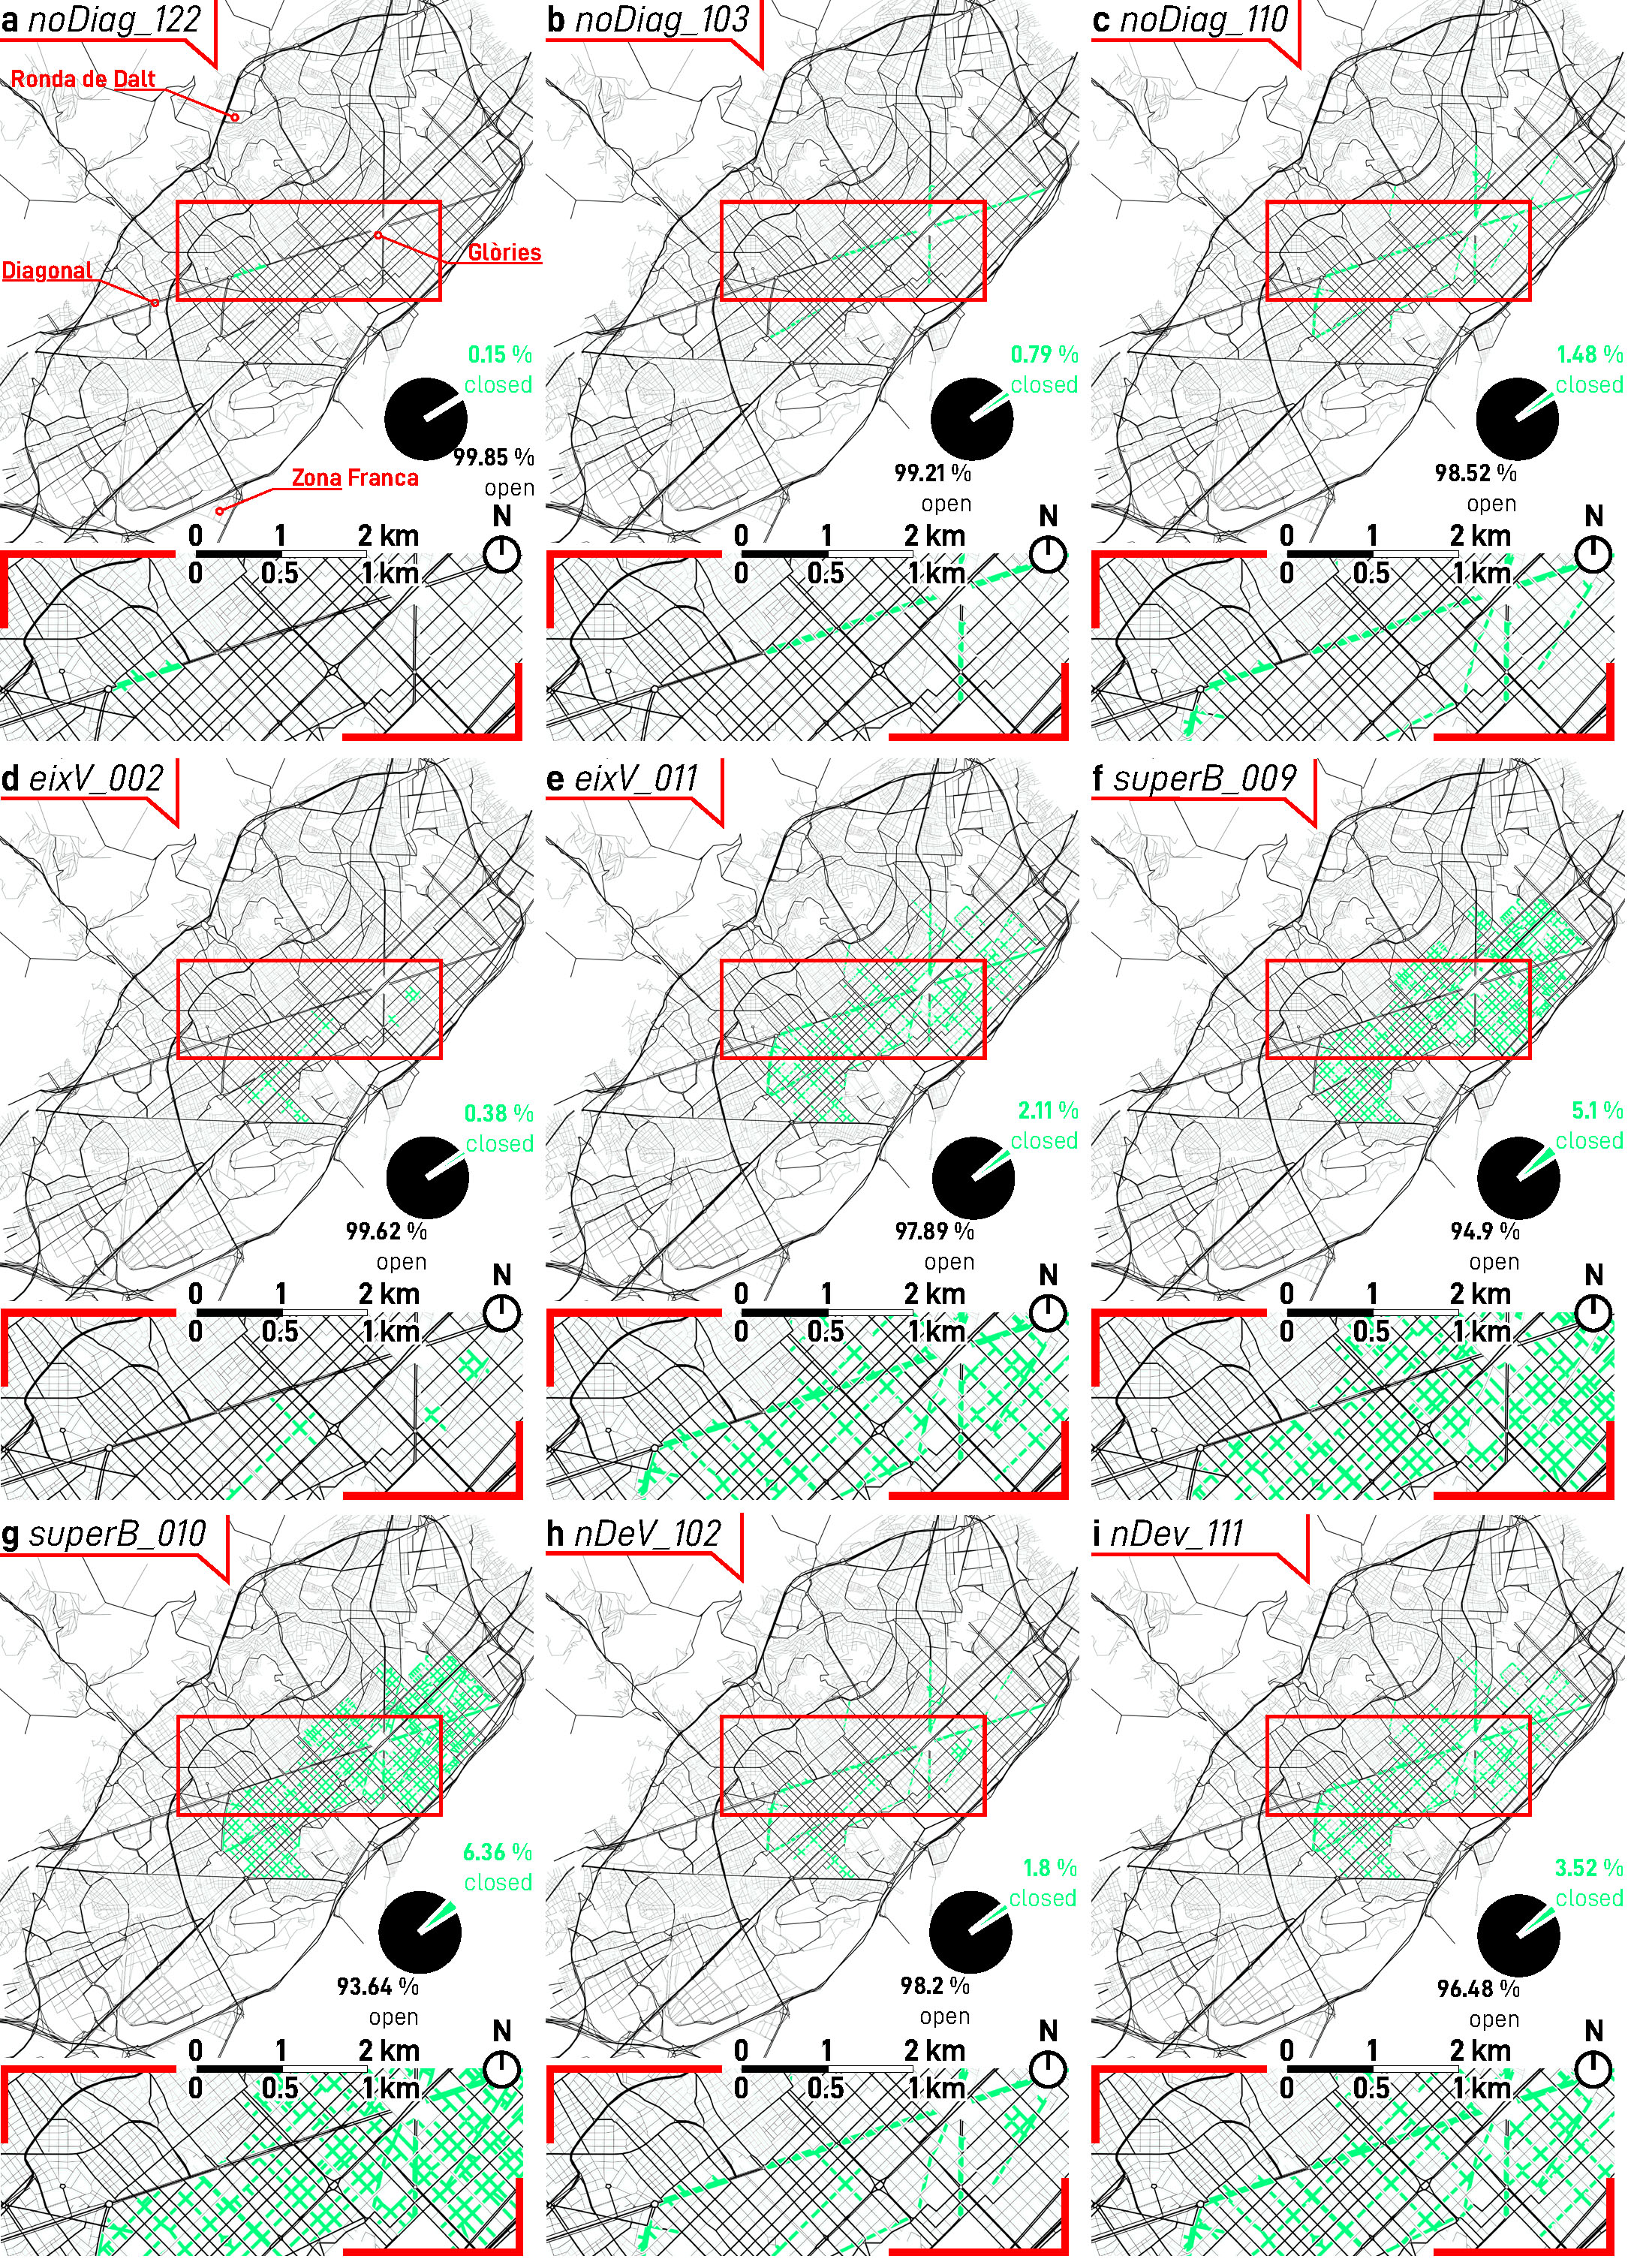
\includegraphics[width=1\textwidth]{LCBM_fig_map_01.jpg}
    \captionsetup{font=scriptsize}
    \caption{City maps of the networks of the analysed alternative scenarios. In green, the closed roadways to traffic are highlighted; in black,  open roadways to general traffic. The rectangles below each subfigure display a zoom of the central part of the city most affected by the various scenarios considered. \emph{Baseline\_000} corresponds to the situation in 2021, without any closed roadway.}
   \label{fig:LCBM_fig_map_01}
\end{figure}

\begin{figure}[htbp!]
    \centering
    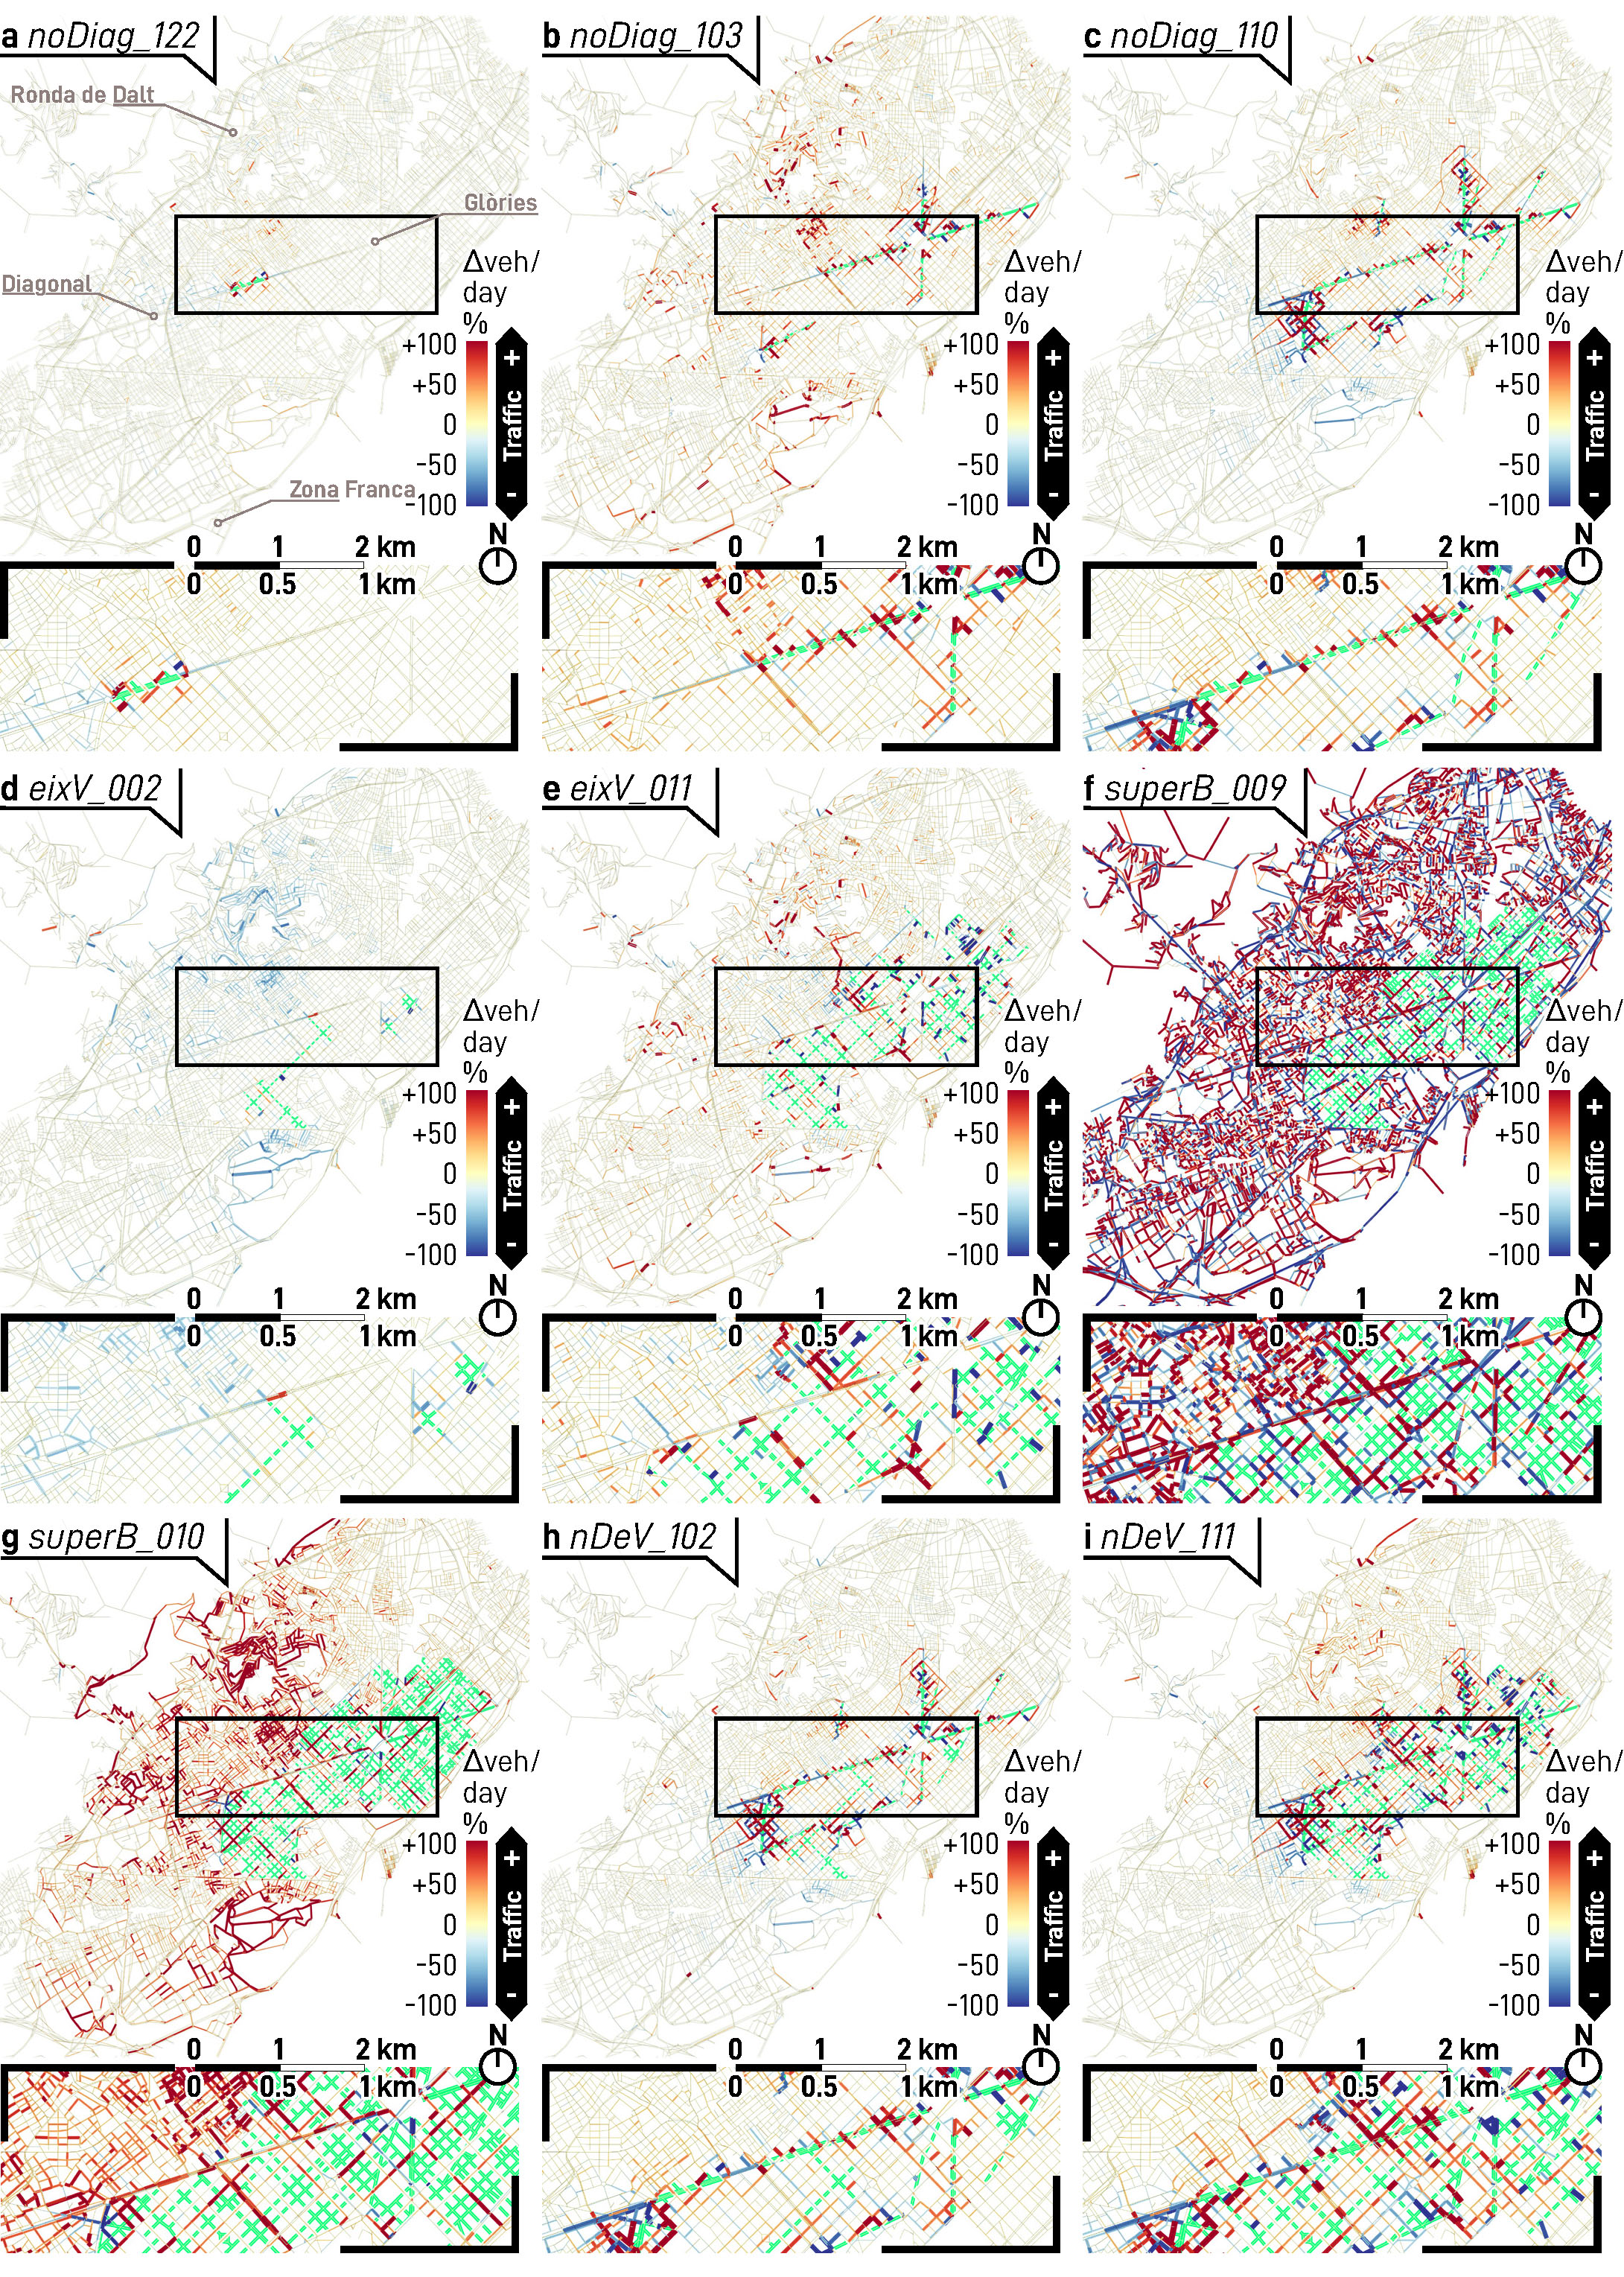
\includegraphics[width=1\textwidth]{LCBM_fig_map_02.jpg}
    \captionsetup{font=scriptsize}
    \caption{Percentage change of average daily traffic counts of the analysed scenarios compared to the baseline. The rectangles below each subfigure display a zoom of the central part of the city of Barcelona. Roadways closed to traffic are illustrated in green.}
   \label{fig:LCBM_fig_map_02}
\end{figure}

\begin{figure}[htbp!]
    \centering
    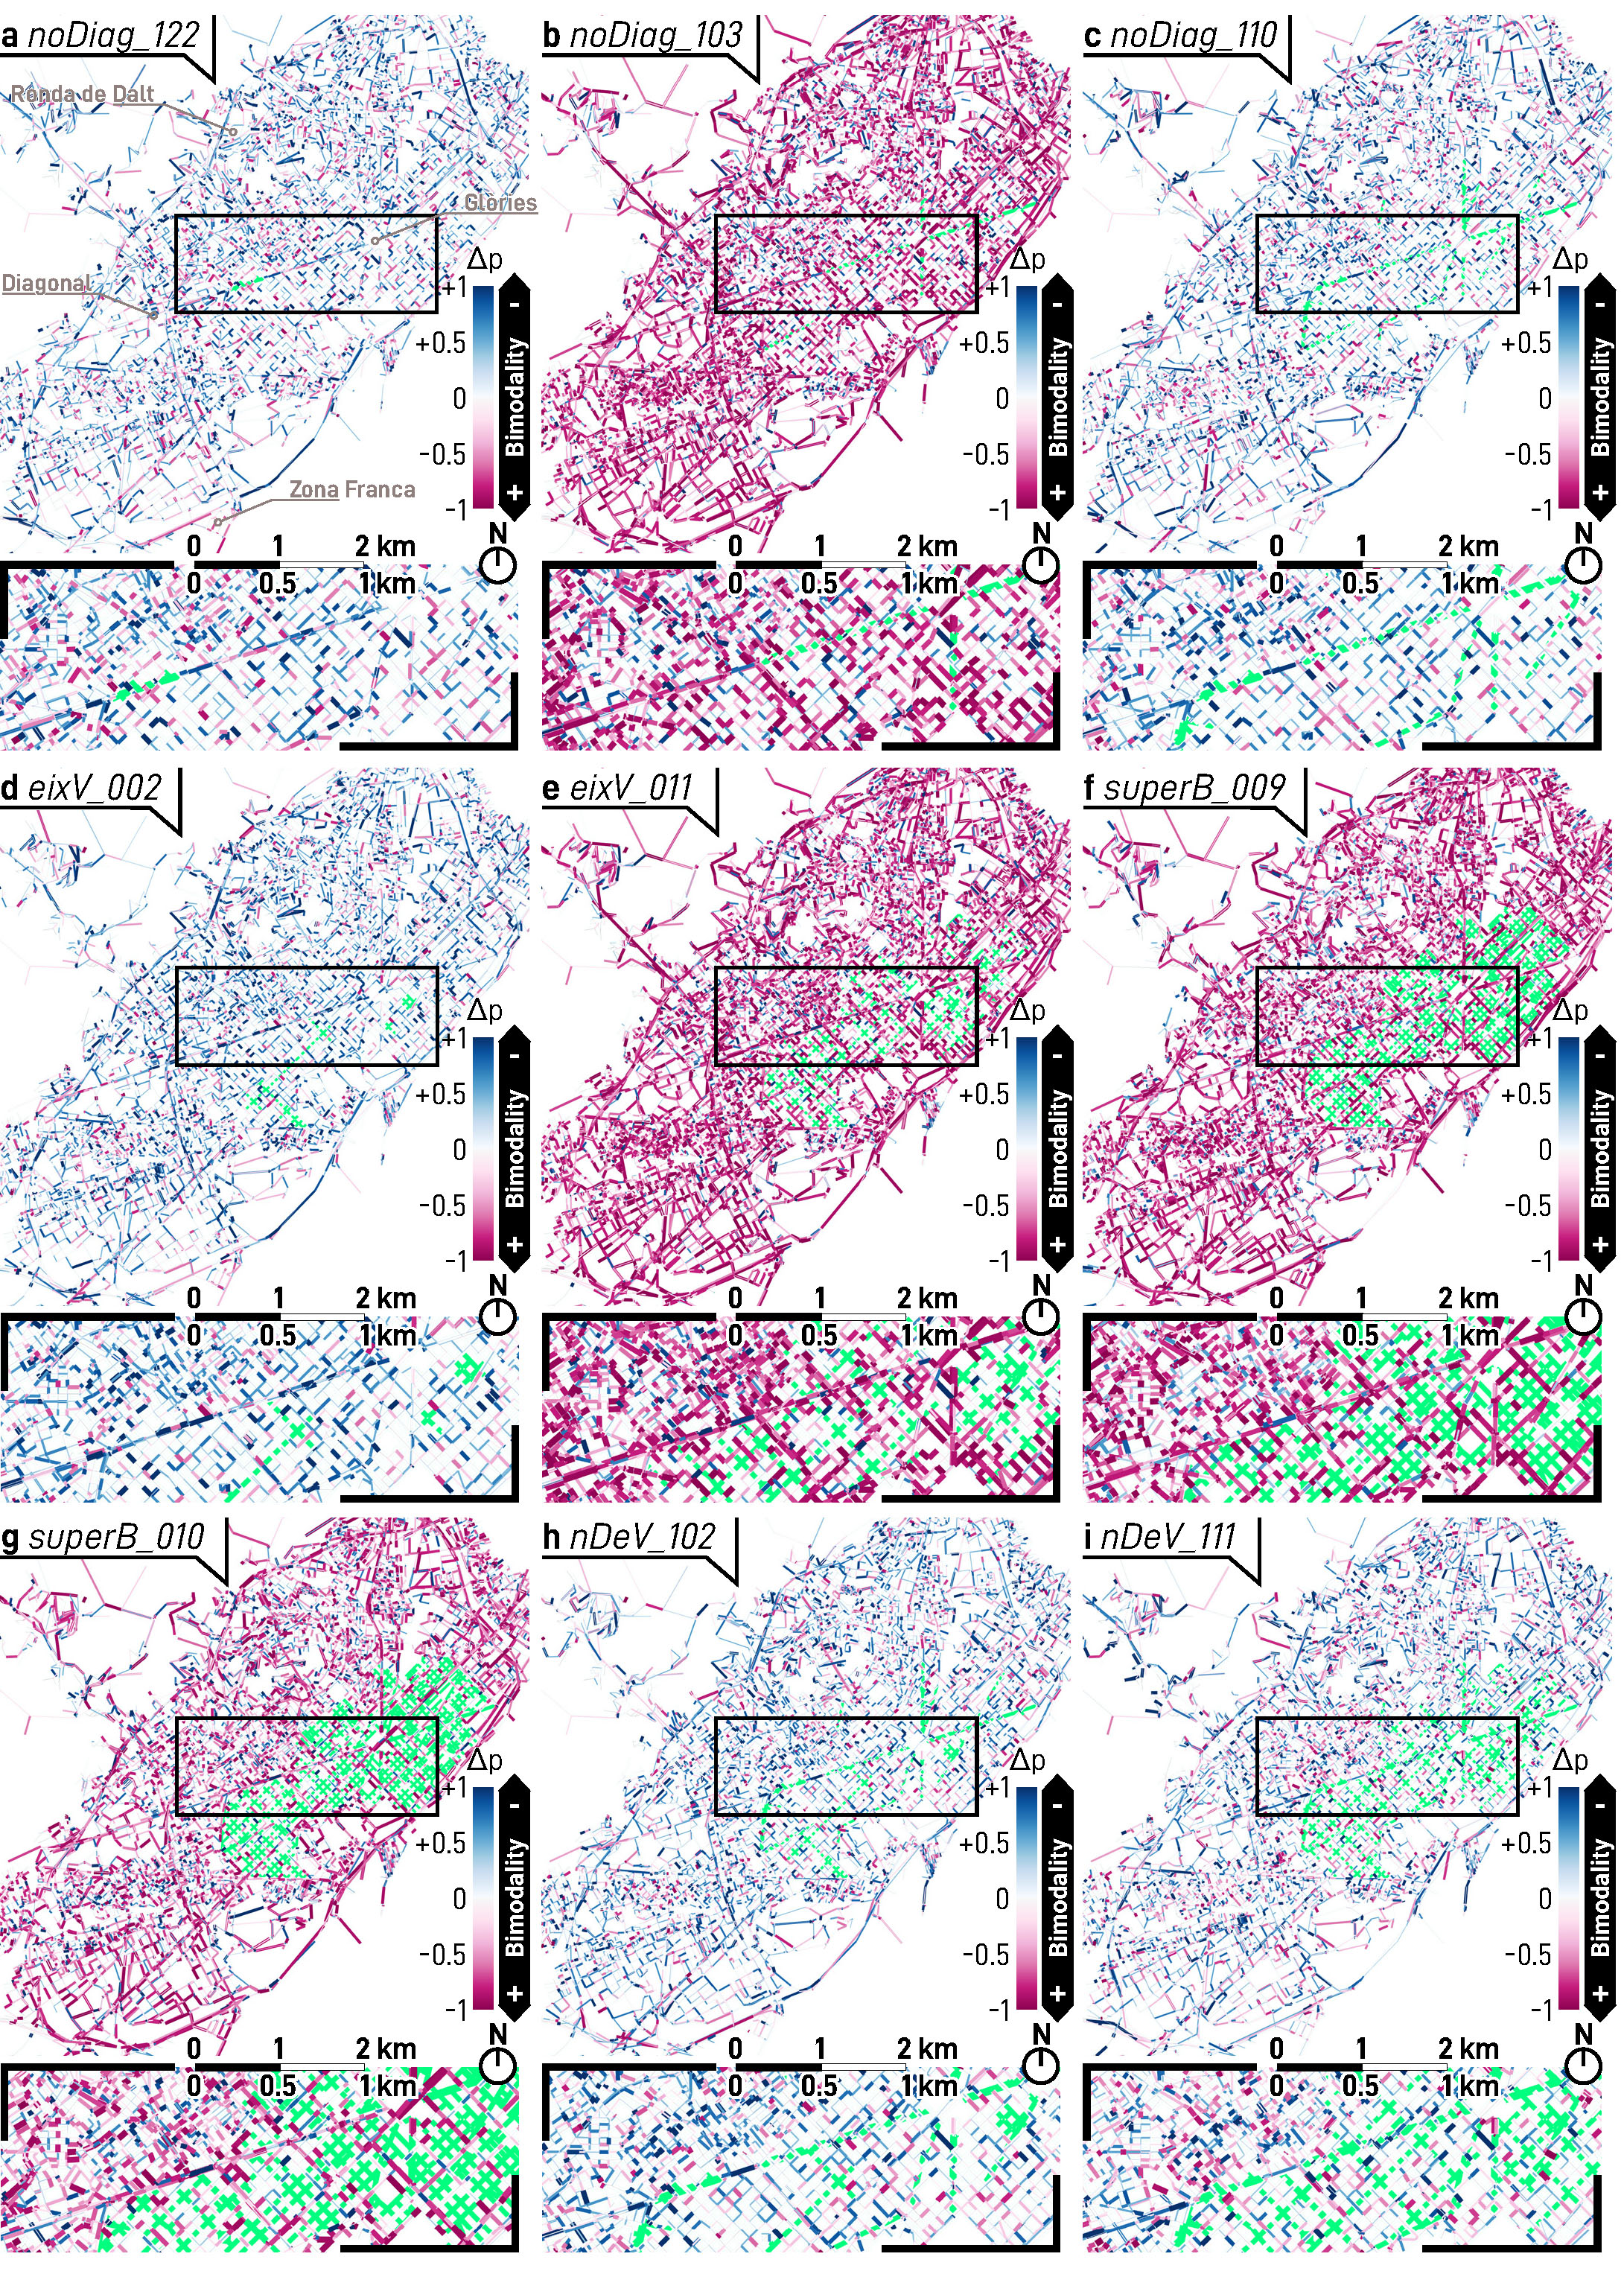
\includegraphics[width=1\textwidth]{LCBM_fig_map_03.jpg}
    \captionsetup{font=scriptsize}
    \caption{Variation of the p-value per edge from Hartigan's Dip test for bimodality applied to travel times of the analysed scenarios compared to the baseline. A lower p-value indicates statistical significance for bimodality (e.g. scenario \emph{eixV\_002} reduces bimodality at the street level). The rectangles below each subfigure display a zoom of the central part of the city of Barcelona. Roadways closed to traffic are illustrated in green.}
   \label{fig:LCBM_fig_map_03}
\end{figure}

\begin{figure}[htbp!]
    \centering
    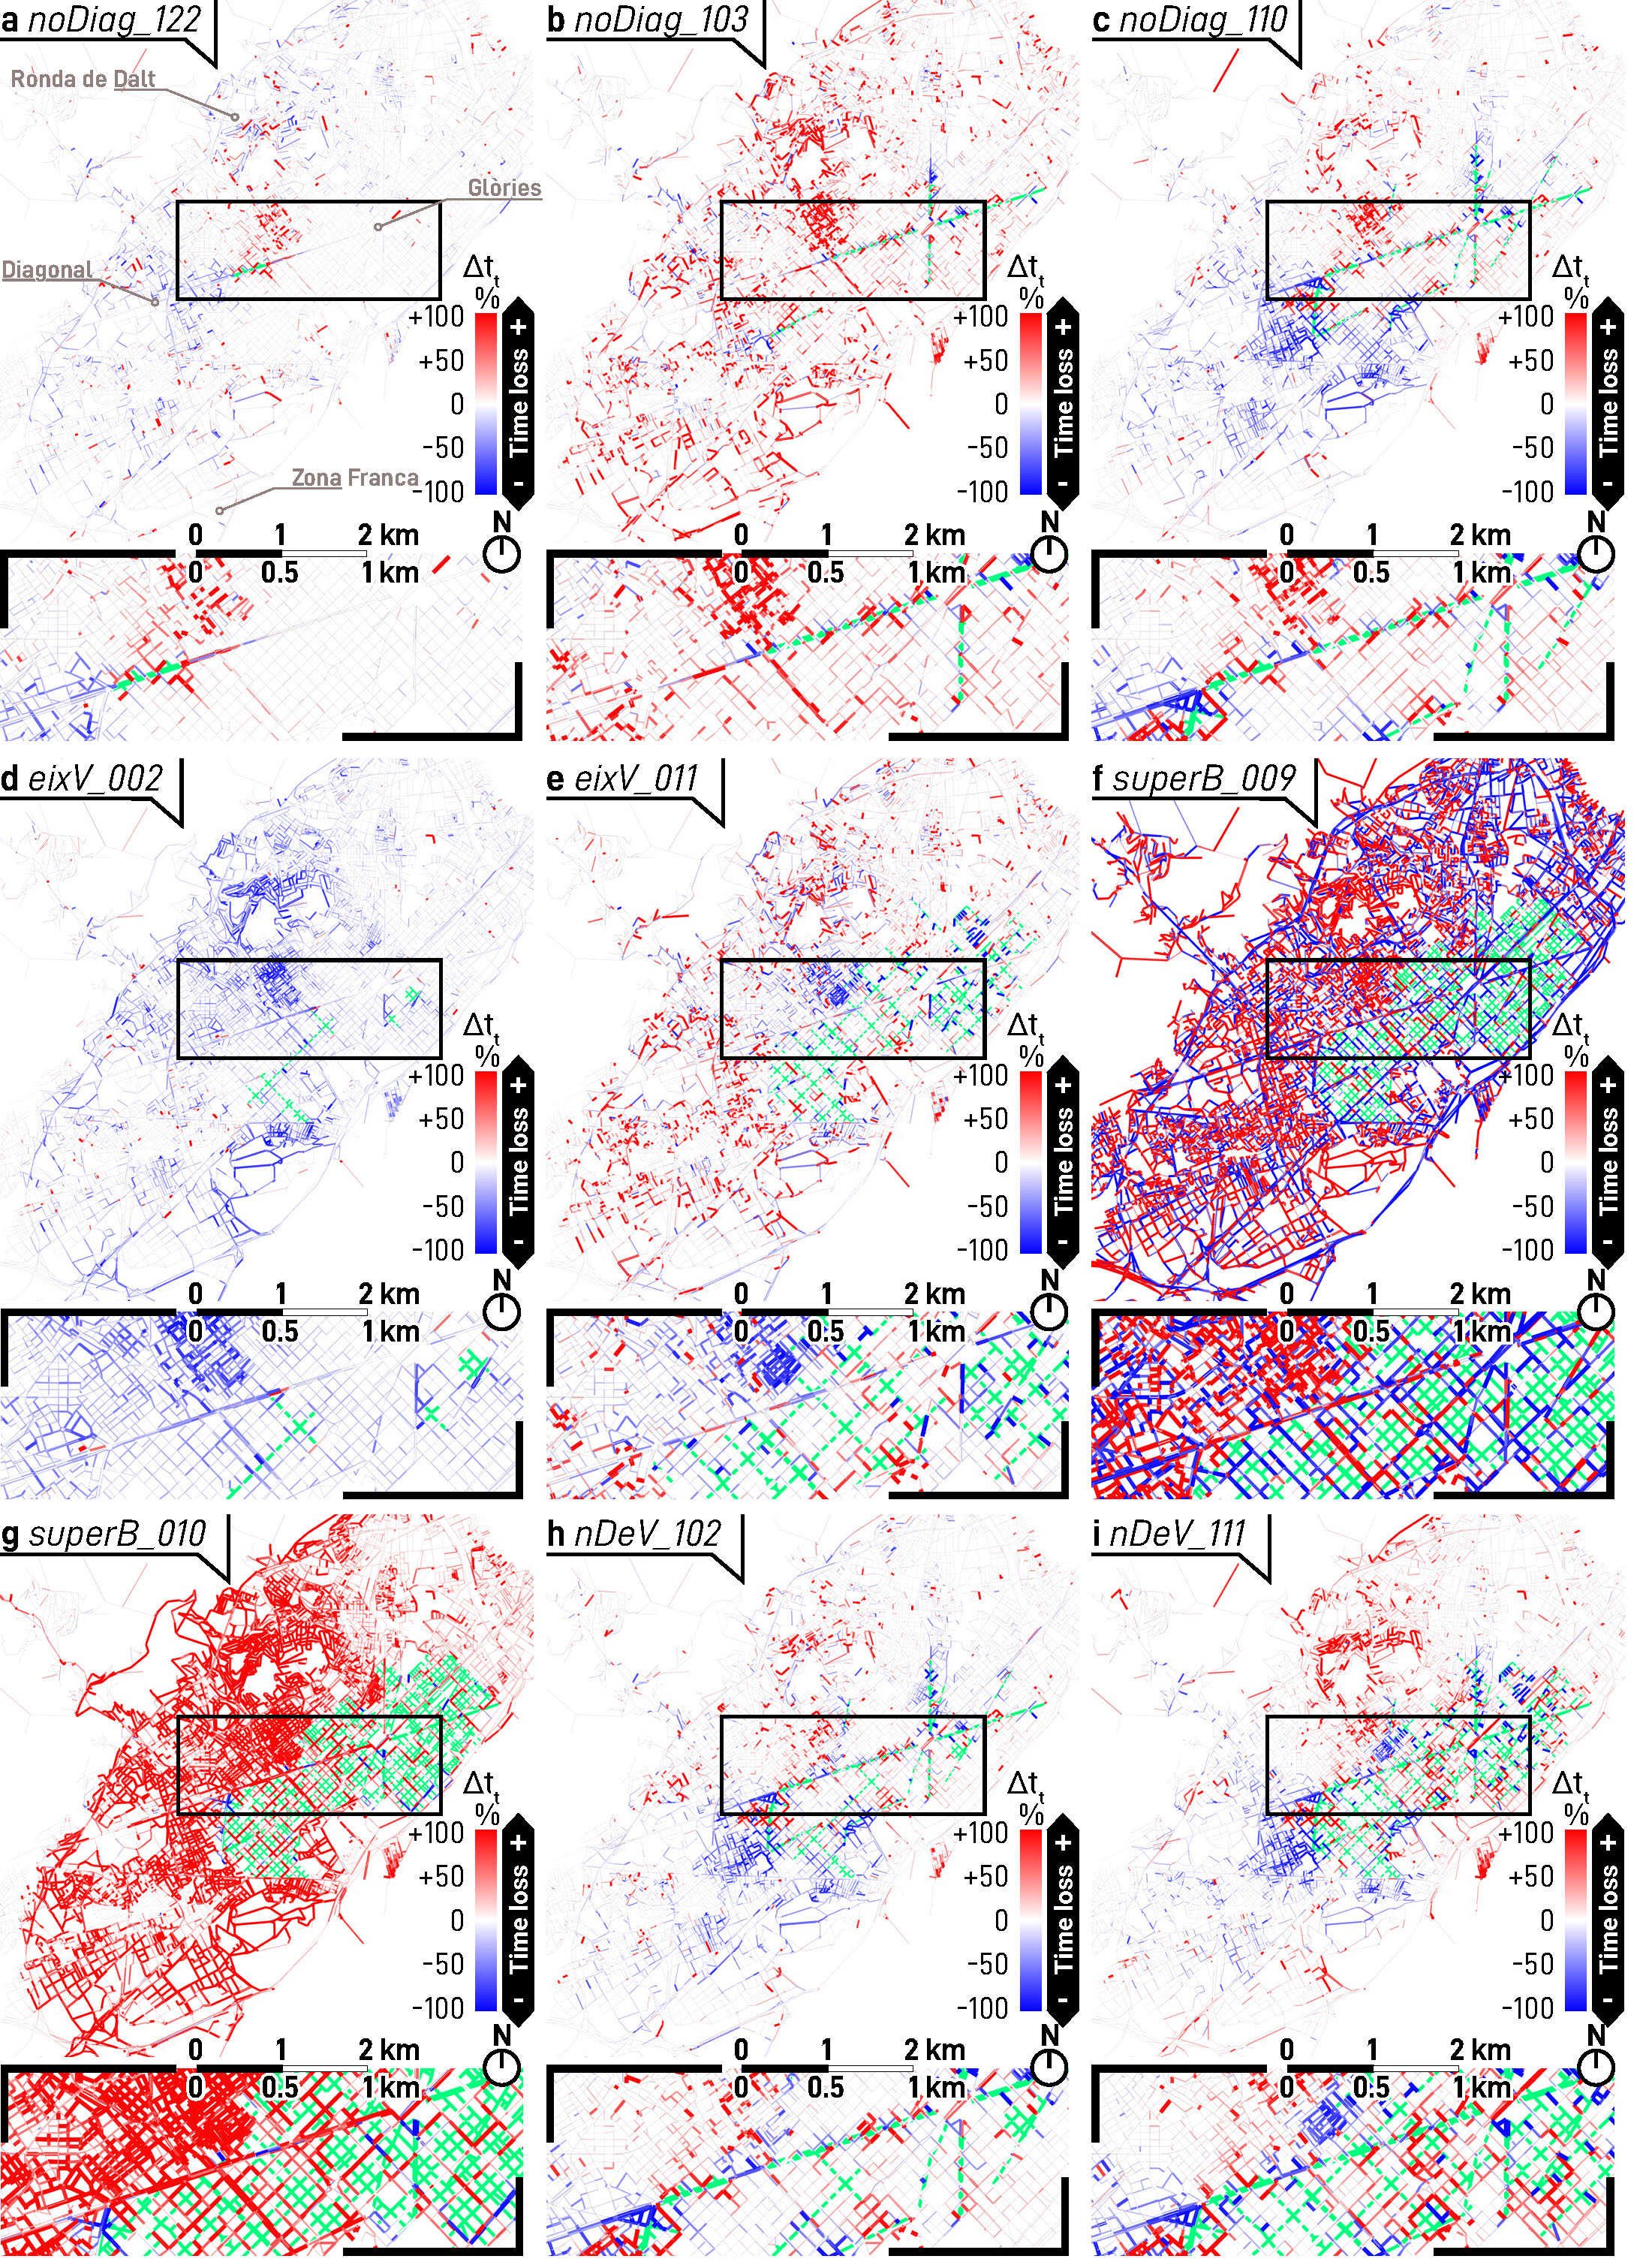
\includegraphics[width=1\textwidth]{LCBM_fig_map_04.jpg}
    \captionsetup{font=scriptsize}
    \caption{Percentage change in median time loss of the analysed scenarios compared to the baseline. The rectangles below each subfigure display a zoom of the central part of the city of Barcelona. Roadways closed to traffic are illustrated in green.}
   \label{fig:LCBM_fig_map_04}
\end{figure}

\begin{figure}[htbp!]
    \centering
    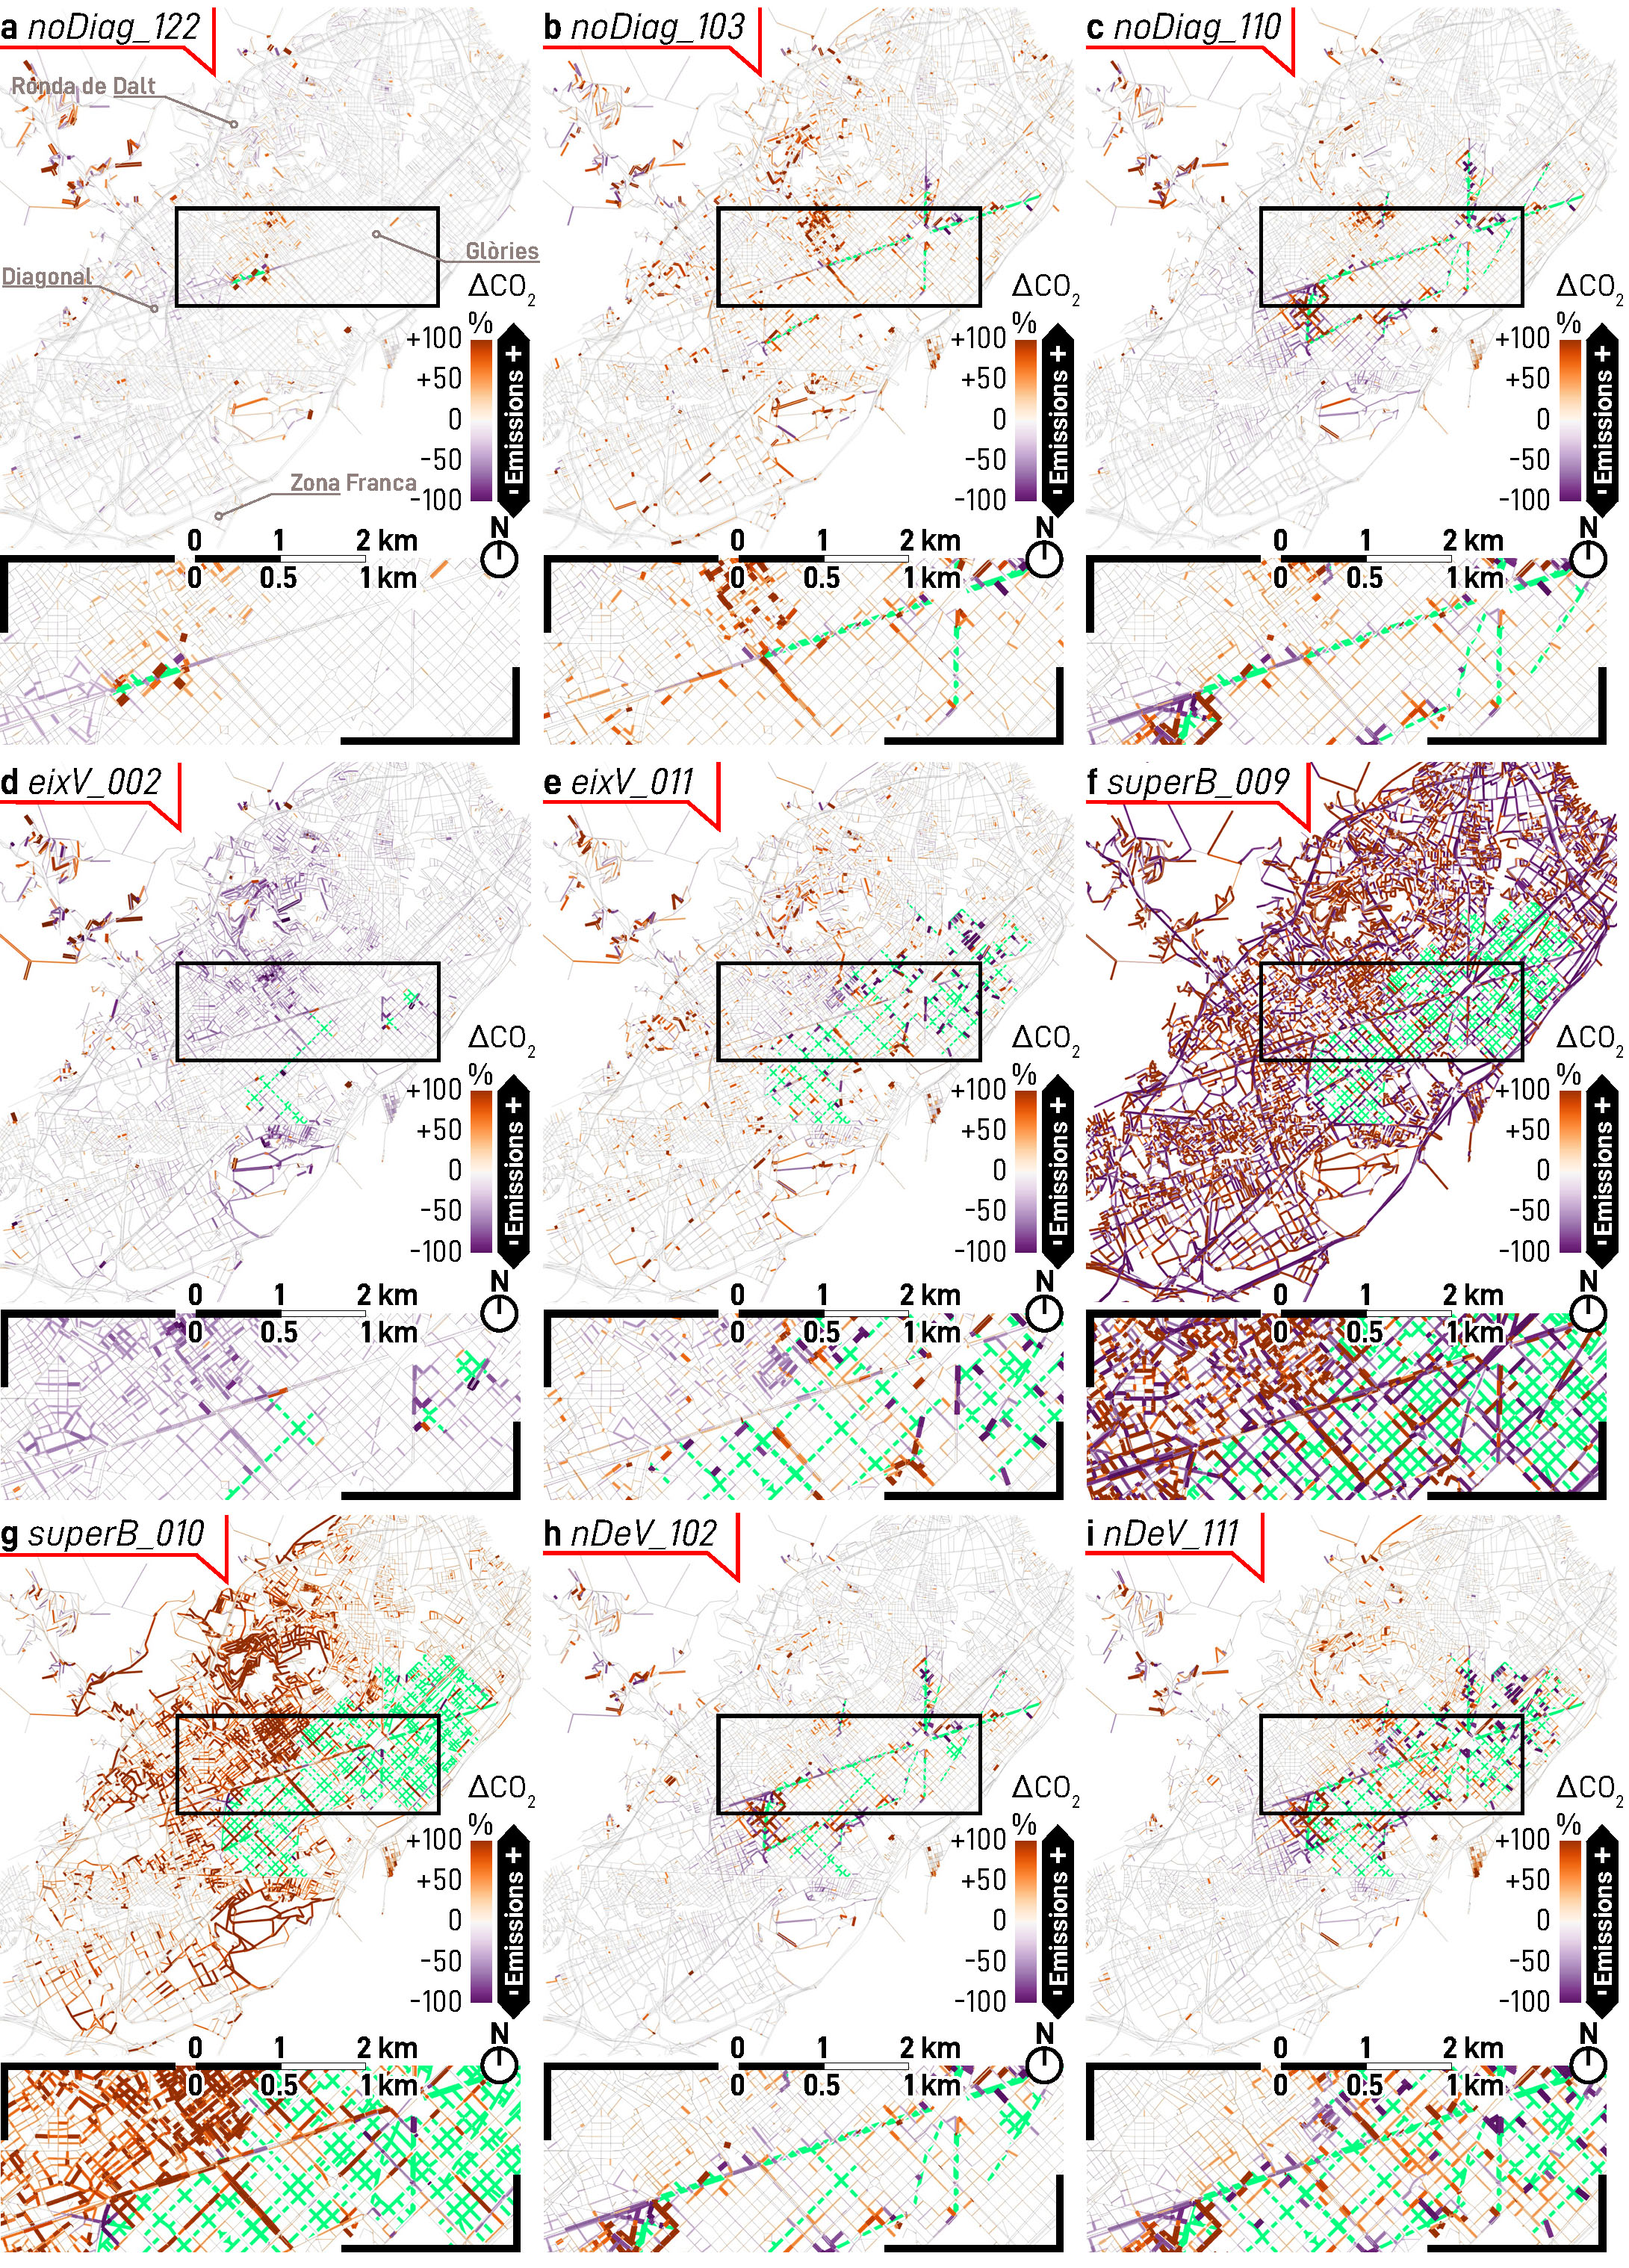
\includegraphics[width=1\textwidth]{LCBM_fig_map_05.jpg}
    \captionsetup{font=scriptsize}
    \caption{Percentage change of median CO\textsubscript{2} emissions per edge of the analysed scenarios compared to the baseline. The rectangles below each subfigure display a zoom of the central part of the city of Barcelona. Roadways closed to traffic are illustrated in green.}
   \label{fig:LCBM_fig_map_05}
\end{figure}

% \chapter{Appendix. Glossary}
% \chaptermark{Appendix. Glossary}
% \label{ch:appendix_LCBM_glossary}
% % \usepackage{tabularray}
\begin{table}
\centering
\resizebox{\linewidth}{!}{%
\begin{tblr}{
}
\textbf{Avg.} & Average                                                               \\
\textbf{CEPs} & Characteristic Emission
  curves over Power                           \\
\textbf{CTM}  & Chemical Transport Model                                              \\
\textbf{CO}   & Carbon
  monoxide                                                     \\
\textbf{CO2}  & Carbon dioxide                                                        \\
\textbf{DLR}  & Deutsches Zentrum für Luft- und
  Raumfahrt (German Aerospace Center) \\
\textbf{DUA}  & Dynamic User Assignment                                               \\
\textbf{DUE}  & Dynamic
  User Equilibrium                                            \\
\textbf{eCDF} & Empirical Cumulative
  Distribution Function                         \\
\textbf{GHG}  & Greenhouse
  Gases                                                    \\
\textbf{HC}   & Carbon hydride                                                        \\
\textbf{iSAR} & in-Simulation Adaptive
  Rerouting                                    \\
\textbf{NOx}  & Nitrogen oxide                                                        \\
\textbf{OSM}  & OpenStreetMap                                                         \\
\textbf{PHEM} & Passenger car and Heavy duty Emission Model                           \\
\textbf{PMx}  & Particulate Matter                                                    \\
\textbf{RMB}  & Regió Metropolitana de
  Barcelona (Metropolitan Region of Barcelona) \\
\textbf{SUMO} & Simulation
  of Urban Mobility                                        
\end{tblr}
}
\end{table}

